%%%%%%%%%%%%%%%%%%%%%%%%%%%%%%%%%%%%%%%%%%%%%%%%%%%%%%%%%%%%%%%%%%%%%%
% Template for a UBC-compliant dissertation
% At the minimum, you will need to change the information found
% after the "Document meta-data"
%
%!TEX TS-program = pdflatex
%!TEX encoding = UTF-8 Unicode

%% The ubcdiss class provides several options:
%%   gpscopy (aka fogscopy)
%%       set parameters to exactly how GPS specifies
%%         * single-sided
%%         * page-numbering starts from title page
%%         * the lists of figures and tables have each entry prefixed
%%           with 'Figure' or 'Table'
%%       This can be tested by `\ifgpscopy ... \else ... \fi'
%%   10pt, 11pt, 12pt
%%       set default font size
%%   oneside, twoside
%%       whether to format for single-sided or double-sided printing
%%   balanced
%%       when double-sided, ensure page content is centred
%%       rather than slightly offset (the default)
%%   singlespacing, onehalfspacing, doublespacing
%%       set default inter-line text spacing; the ubcdiss class
%%       provides \textspacing to revert to this configured spacing
%%   draft
%%       disable more intensive processing, such as including
%%       graphics, etc.
%%

% For submission to GPS
\documentclass[gpscopy,onehalfspacing,11pt]{ubcdiss}

% For your own copies (looks nicer)
% \documentclass[balanced,twoside,11pt]{ubcdiss}

%%%%%%%%%%%%%%%%%%%%%%%%%%%%%%%%%%%%%%%%%%%%%%%%%%%%%%%%%%%%%%%%%%%%%%
%%%%%%%%%%%%%%%%%%%%%%%%%%%%%%%%%%%%%%%%%%%%%%%%%%%%%%%%%%%%%%%%%%%%%%
%%
%% FONTS:
%% 
%% The defaults below configures Times Roman for the serif font,
%% Helvetica for the sans serif font, and Courier for the
%% typewriter-style font.  Configuring fonts can be time
%% consuming; we recommend skipping to END FONTS!
%% 
%% If you're feeling brave, have lots of time, and wish to use one
%% your platform's native fonts, see the commented out bits below for
%% XeTeX/XeLaTeX.  This is not for the faint at heart. 
%% (And shouldn't you be writing? :-)
%%

%% NFSS font specification (New Font Selection Scheme)
\usepackage{times,mathptmx,courier}
\usepackage[scaled=.92]{helvet}

%% Math or theory people may want to include the handy AMS macros
%\usepackage{amssymb}
%\usepackage{amsmath}
%\usepackage{amsfonts}

%% The pifont package provides access to the elements in the dingbat font.   
%% Use \ding{##} for a particular dingbat (see p7 of psnfss2e.pdf)
%%   Useful:
%%     51,52 different forms of a checkmark
%%     54,55,56 different forms of a cross (saltyre)
%%     172-181 are 1-10 in open circle (serif)
%%     182-191 are 1-10 black circle (serif)
%%     192-201 are 1-10 in open circle (sans serif)
%%     202-211 are 1-10 in black circle (sans serif)
%% \begin{dinglist}{##}\item... or dingautolist (which auto-increments)
%% to create a bullet list with the provided character.
\usepackage{pifont}

%%%%%%%%%%%%%%%%%%%%%%%%%%%%%%%%%%%%%%%%%%%%%%%%%%%%%%%%%%%%%%%%%%%%%%
%% Configure fonts for XeTeX / XeLaTeX using the fontspec package.
%% Be sure to check out the fontspec documentation.
%\usepackage{fontspec,xltxtra,xunicode}	% required
%\defaultfontfeatures{Mapping=tex-text}	% recommended
%% Minion Pro and Myriad Pro are shipped with some versions of
%% Adobe Reader.  Adobe representatives have commented that these
%% fonts can be used outside of Adobe Reader.
%\setromanfont[Numbers=OldStyle]{Minion Pro}
%\setsansfont[Numbers=OldStyle,Scale=MatchLowercase]{Myriad Pro}
%\setmonofont[Scale=MatchLowercase]{Andale Mono}

%% Other alternatives:
%\setromanfont[Mapping=tex-text]{Adobe Caslon}
%\setsansfont[Scale=MatchLowercase]{Gill Sans}
%\setsansfont[Scale=MatchLowercase,Mapping=tex-text]{Futura}
%\setmonofont[Scale=MatchLowercase]{Andale Mono}
%\newfontfamily{\SYM}[Scale=0.9]{Zapf Dingbats}
%% END FONTS
%%%%%%%%%%%%%%%%%%%%%%%%%%%%%%%%%%%%%%%%%%%%%%%%%%%%%%%%%%%%%%%%%%%%%%
%%%%%%%%%%%%%%%%%%%%%%%%%%%%%%%%%%%%%%%%%%%%%%%%%%%%%%%%%%%%%%%%%%%%%%



%%%%%%%%%%%%%%%%%%%%%%%%%%%%%%%%%%%%%%%%%%%%%%%%%%%%%%%%%%%%%%%%%%%%%%
%%%%%%%%%%%%%%%%%%%%%%%%%%%%%%%%%%%%%%%%%%%%%%%%%%%%%%%%%%%%%%%%%%%%%%
%%
%% Recommended packages
%%
\usepackage{checkend}	% better error messages on left-open environments
\usepackage{graphicx}	% for incorporating external images
\graphicspath{ {img/} } % images are kept in a folder named img under the current directory

%% booktabs: provides some special commands for typesetting tables as used
%% in excellent journals.  Ignore the examples in the Lamport book!
\usepackage{booktabs}

%% listings: useful support for including source code listings, with
%% optional special keyword formatting.  The \lstset{} causes
%% the text to be typeset in a smaller sans serif font, with
%% proportional spacing.
\usepackage{listings}
\lstset{basicstyle=\sffamily\scriptsize,showstringspaces=false,fontadjust}

%% The acronym package provides support for defining acronyms, providing
%% their expansion when first used, and building glossaries.  See the
%% example in glossary.tex and the example usage throughout the example
%% document.
%% NOTE: to use \MakeTextLowercase in the \acsfont command below,
%%   we *must* use the `nohyperlinks' option -- it causes errors with
%%   hyperref otherwise.  See Section 5.2 in the ``LaTeX 2e for Class
%%   and Package Writers Guide'' (clsguide.pdf) for details.
\usepackage[printonlyused,nohyperlinks]{acronym}
%% The ubcdiss.cls loads the `textcase' package which provides commands
%% for upper-casing and lower-casing text.  The following causes
%% the acronym package to typeset acronyms in small-caps
%% as recommended by Bringhurst.
\renewcommand{\acsfont}[1]{{\scshape \MakeTextLowercase{#1}}}

%% color: add support for expressing colour models.  Grey can be used
%% to great effect to emphasize other parts of a graphic or text.
%% For an excellent set of examples, see Tufte's "Visual Display of
%% Quantitative Information" or "Envisioning Information".
\usepackage{color}
\definecolor{greytext}{gray}{0.5}

%% comment: provides a new {comment} environment: all text inside the
%% environment is ignored.
%%   \begin{comment} ignored text ... \end{comment}
\usepackage{comment}

%% The natbib package provides more sophisticated citing commands
%% such as \citeauthor{} to provide the author names of a work,
%% \citet{} to produce an author-and-reference citation,
%% \citep{} to produce a parenthetical citation.
%% We use \citeeg{} to provide examples
\usepackage[numbers,sort&compress]{natbib}
\newcommand{\citeeg}[1]{\citep[e.g.,][]{#1}}

%% The titlesec package provides commands to vary how chapter and
%% section titles are typeset.  The following uses more compact
%% spacings above and below the title.  The titleformat that follow
%% ensure chapter/section titles are set in singlespace.
\usepackage[compact]{titlesec}
\titleformat*{\section}{\singlespacing\raggedright\bfseries\Large}
\titleformat*{\subsection}{\singlespacing\raggedright\bfseries\large}
\titleformat*{\subsubsection}{\singlespacing\raggedright\bfseries}
\titleformat*{\paragraph}{\singlespacing\raggedright\itshape}

%% The caption package provides support for varying how table and
%% figure captions are typeset.
\usepackage[format=hang,indention=-1cm,labelfont={bf},margin=1em]{caption}

%% url: for typesetting URLs and smart(er) hyphenation.
%% \url{http://...} 
\usepackage{url}
\urlstyle{sf}	% typeset urls in sans-serif


%%%%%%%%%%%%%%%%%%%%%%%%%%%%%%%%%%%%%%%%%%%%%%%%%%%%%%%%%%%%%%%%%%%%%%
%%%%%%%%%%%%%%%%%%%%%%%%%%%%%%%%%%%%%%%%%%%%%%%%%%%%%%%%%%%%%%%%%%%%%%
%%
%% Possibly useful packages: you may need to explicitly install
%% these from CTAN if they aren't part of your distribution;
%% teTeX seems to ship with a smaller base than MikTeX and MacTeX.
%%
%\usepackage{pdfpages}	% insert pages from other PDF files
%\usepackage{longtable}	% provide tables spanning multiple pages
%\usepackage{chngpage}	% support changing the page widths on demand
%\usepackage{tabularx}	% an enhanced tabular environment

%% enumitem: support pausing and resuming enumerate environments.
%\usepackage{enumitem}

%% rotating: provides two environments, sidewaystable and sidewaysfigure,
%% for typesetting tables and figures in landscape mode.  
%\usepackage{rotating}

%% subfig: provides for including subfigures within a figure,
%% and includes being able to separately reference the subfigures.
%\usepackage{subfig}

%% graph: provides capabilities to draw graphs
\usepackage{tikz}

%% ragged2e: provides several new new commands \Centering, \RaggedLeft,
%% \RaggedRight and \justifying and new environments Center, FlushLeft,
%% FlushRight and justify, which set ragged text and are easily
%% configurable to allow hyphenation.
%\usepackage{ragged2e}

%% The ulem package provides a \sout{} for striking out text and
%% \xout for crossing out text.  The normalem and normalbf are
%% necessary as the package messes with the emphasis and bold fonts
%% otherwise.
%\usepackage[normalem,normalbf]{ulem}    % for \sout

%%%%%%%%%%%%%%%%%%%%%%%%%%%%%%%%%%%%%%%%%%%%%%%%%%%%%%%%%%%%%%%%%%%%%%
%% HYPERREF:
%% The hyperref package provides for embedding hyperlinks into your
%% document.  By default the table of contents, references, citations,
%% and footnotes are hyperlinked.
%%
%% Hyperref provides a very handy command for doing cross-references:
%% \autoref{}.  This is similar to \ref{} and \pageref{} except that
%% it automagically puts in the *type* of reference.  For example,
%% referencing a figure's label will put the text `Figure 3.4'.
%% And the text will be hyperlinked to the appropriate place in the
%% document.
%%
%% Generally hyperref should appear after most other packages

%% The following puts hyperlinks in very faint grey boxes.
%% The `pagebackref' causes the references in the bibliography to have
%% back-references to the citing page; `backref' puts the citing section
%% number.  See further below for other examples of using hyperref.
%% 2009/12/09: now use `linktocpage' (Jacek Kisynski): GPS now prefers
%%   that the ToC, LoF, LoT place the hyperlink on the page number,
%%   rather than the entry text.
\usepackage[bookmarks,bookmarksnumbered,%
    allbordercolors={0.8 0.8 0.8},%
    pagebackref,linktocpage%
    ]{hyperref}
%% The following change how the the back-references text is typeset in a
%% bibliography when `backref' or `pagebackref' are used
\renewcommand\backrefpagesname{\(\rightarrow\) pages}
\renewcommand\backref{\textcolor{greytext} \backrefpagesname\ }

%% The following uses most defaults, which causes hyperlinks to be
%% surrounded by colourful boxes; the colours are only visible in
%% PDFs and don't show up when printed:
%\usepackage[bookmarks,bookmarksnumbered]{hyperref}

%% The following disables the colourful boxes around hyperlinks.
%\usepackage[bookmarks,bookmarksnumbered,pdfborder={0 0 0}]{hyperref}

%% The following disables all hyperlinking, but still enabled use of
%% \autoref{}
%\usepackage[draft]{hyperref}

%% The following commands causes chapter and section references to
%% uppercase the part name.
\renewcommand{\chapterautorefname}{Chapter}
\renewcommand{\sectionautorefname}{Section}
\renewcommand{\subsectionautorefname}{Section}
\renewcommand{\subsubsectionautorefname}{Section}

%% If you have long page numbers (e.g., roman numbers in the 
%% preliminary pages for page 28 = xxviii), you might need to
%% uncomment the following and tweak the \@pnumwidth length
%% (default: 1.55em).  See the tocloft documentation at
%% http://www.ctan.org/tex-archive/macros/latex/contrib/tocloft/
% \makeatletter
% \renewcommand{\@pnumwidth}{3em}
% \makeatother

%%%%%%%%%%%%%%%%%%%%%%%%%%%%%%%%%%%%%%%%%%%%%%%%%%%%%%%%%%%%%%%%%%%%%%
%%%%%%%%%%%%%%%%%%%%%%%%%%%%%%%%%%%%%%%%%%%%%%%%%%%%%%%%%%%%%%%%%%%%%%
%%
%% Some special settings that controls how text is typeset
%%
% \raggedbottom		% pages don't have to line up nicely on the last line
% \sloppy		% be a bit more relaxed in inter-word spacing
% \clubpenalty=10000	% try harder to avoid orphans
% \widowpenalty=10000	% try harder to avoid widows
% \tolerance=1000

%% And include some of our own useful macros
% This file provides examples of some useful macros for typesetting
% dissertations.  None of the macros defined here are necessary beyond
% for the template documentation, so feel free to change, remove, and add
% your own definitions.
%
% We recommend that you define macros to separate the semantics
% of the things you write from how they are presented.  For example,
% you'll see definitions below for a macro \file{}: by using
% \file{} consistently in the text, we can change how filenames
% are typeset simply by changing the definition of \file{} in
% this file.
% 
%% The following is a directive for TeXShop to indicate the main file
%%!TEX root = diss.tex

\newcommand{\NA}{\textsc{n/a}}	% for "not applicable"
\newcommand{\eg}{e.g.,\ }	% proper form of examples (\eg a, b, c)
\newcommand{\ie}{i.e.,\ }	% proper form for that is (\ie a, b, c)
\newcommand{\etal}{\emph{et al}}

% Some useful macros for typesetting terms.
\newcommand{\file}[1]{\texttt{#1}}
\newcommand{\class}[1]{\texttt{#1}}
\newcommand{\latexpackage}[1]{\href{http://www.ctan.org/macros/latex/contrib/#1}{\texttt{#1}}}
\newcommand{\latexmiscpackage}[1]{\href{http://www.ctan.org/macros/latex/contrib/misc/#1.sty}{\texttt{#1}}}
\newcommand{\env}[1]{\texttt{#1}}
\newcommand{\BibTeX}{Bib\TeX}

% Define a command \doi{} to typeset a digital object identifier (DOI).
% Note: if the following definition raise an error, then you likely
% have an ancient version of url.sty.  Either find a more recent version
% (3.1 or later work fine) and simply copy it into this directory,  or
% comment out the following two lines and uncomment the third.
\DeclareUrlCommand\DOI{}
\newcommand{\doi}[1]{\href{http://dx.doi.org/#1}{\DOI{doi:#1}}}
%\newcommand{\doi}[1]{\href{http://dx.doi.org/#1}{doi:#1}}

% Useful macro to reference an online document with a hyperlink
% as well with the URL explicitly listed in a footnote
% #1: the URL
% #2: the anchoring text
\newcommand{\webref}[2]{\href{#1}{#2}\footnote{\url{#1}}}

% epigraph is a nice environment for typesetting quotations
\makeatletter
\newenvironment{epigraph}{%
	\begin{flushright}
	\begin{minipage}{\columnwidth-0.75in}
	\begin{flushright}
	\@ifundefined{singlespacing}{}{\singlespacing}%
    }{
	\end{flushright}
	\end{minipage}
	\end{flushright}}
\makeatother

% \FIXME{} is a useful macro for noting things needing to be changed.
% The following definition will also output a warning to the console
\newcommand{\FIXME}[1]{\typeout{**FIXME** #1}\textbf{[FIXME: #1]}}

% END


%%%%%%%%%%%%%%%%%%%%%%%%%%%%%%%%%%%%%%%%%%%%%%%%%%%%%%%%%%%%%%%%%%%%%%
%%%%%%%%%%%%%%%%%%%%%%%%%%%%%%%%%%%%%%%%%%%%%%%%%%%%%%%%%%%%%%%%%%%%%%
%%
%% Document meta-data: be sure to also change the \hypersetup information
%%

\title{3D Reconstruction for Everyday Things}
%\subtitle{If you want a subtitle}

\author{Kai Wu}
\previousdegree{Bachelor of Engineering, Beijing University of Posts and Telecommunications 2014}

% What is this dissertation for?
\degreetitle{Master of Applied Science}

\institution{The University of British Columbia}
\campus{Vancouver}

\faculty{The Faculty of Applied Science}
\department{Electric and Computer Engineering Department}
\submissionmonth{April}
\submissionyear{2017}

%% hyperref package provides support for embedding meta-data in .PDF
%% files
\hypersetup{
  pdftitle={Change this title!  (DRAFT: \today)},
  pdfauthor={Johnny Canuck},
  pdfkeywords={Your keywords here}
}

%%%%%%%%%%%%%%%%%%%%%%%%%%%%%%%%%%%%%%%%%%%%%%%%%%%%%%%%%%%%%%%%%%%%%%
%%%%%%%%%%%%%%%%%%%%%%%%%%%%%%%%%%%%%%%%%%%%%%%%%%%%%%%%%%%%%%%%%%%%%%
%% 
%% The document content
%%

%% LaTeX's \includeonly commands causes any uses of \include{} to only
%% include files that are in the list.  This is helpful to produce
%% subsets of your thesis (e.g., for committee members who want to see
%% the dissertation chapter by chapter).  It also saves time by 
%% avoiding reprocessing the entire file.
%\includeonly{intro,conclusions}
%\includeonly{discussion}

\begin{document}

%%%%%%%%%%%%%%%%%%%%%%%%%%%%%%%%%%%%%%%%%%%%%%%%%%
%% From Thesis Components: Tradtional Thesis
%% <http://www.grad.ubc.ca/current-students/dissertation-thesis-preparation/order-components>

% Preliminary Pages (numbered in lower case Roman numerals)
%    1. Title page (mandatory)
\maketitle

%    2. Abstract (mandatory - maximum 350 words)
%% The following is a directive for TeXShop to indicate the main file
%%!TEX root = diss.tex

\chapter{Abstract}

Advancements in state-of-the-art 3D reconstruction algorithms have sped ahead of the development of interfaces or application programming interfaces (APIs) for developers, especially to those who are not experts in computer vision.

We have designed a novel interface, specifically for 3D reconstruction techniques, which uses a description (covering the conditions of the problem) to allow a user to reconstruct the shape of an object without knowledge of 3D vision algorithms. The interface hides the details of algorithms by using a description of visual and geometric properties of the object. Our interface interprets the description and chooses from a set of algorithms those that satisfy the description. We show that this description can be interpreted to one appropriate algorithm, which can give a successful reconstruction result.

We evaluate the interface through a proof-of-concept interpreter, which interprets the description and invokes one of three underlying algorithms for reconstruction. We demonstrate the link between the description set by the user and the result returned using synthetic and real-world datasets where each object has been imaged with the appropriate setup.

\cleardoublepage

%    3. Preface
%% The following is a directive for TeXShop to indicate the main file
%%!TEX root = diss.tex

\chapter{Preface}

The entire work presented here has been done by the author, Kai Wu, with the collaboration and supervision of Dr. Sidney Fels and Dr. Gregor Miller. A manuscript describing the core of our work and our results has been submitted to a vision conference and is under anonymous review at the moment of thesis submission.

\cleardoublepage

%    4. Table of contents (mandatory - list all items in the preliminary pages
%    starting with the abstract, followed by chapter headings and
%    subheadings, bibliographies and appendices)
\tableofcontents
\cleardoublepage	% required by tocloft package

%    5. List of tables (mandatory if thesis has tables)
\listoftables
\cleardoublepage	% required by tocloft package

%    6. List of figures (mandatory if thesis has figures)
\listoffigures
\cleardoublepage	% required by tocloft package

%    7. List of illustrations (mandatory if thesis has illustrations)
%    8. Lists of symbols, abbreviations or other (optional)

%    9. Glossary (optional)
%% The following is a directive for TeXShop to indicate the main file
%%!TEX root = diss.tex

\chapter{Glossary}

This glossary uses the handy \latexpackage{acroynym} package to automatically
maintain the glossary.  It uses the package's \texttt{printonlyused}
option to include only those acronyms explicitly referenced in the
\LaTeX\ source.

% use \acrodef to define an acronym, but no listing
\acrodef{UI}{user interface}
\acrodef{UBC}{University of British Columbia}

% The acronym environment will typeset only those acronyms that were
% *actually used* in the course of the document
\begin{acronym}[ANOVA]
\acro{ANOVA}[ANOVA]{Analysis of Variance\acroextra{, a set of
  statistical techniques to identify sources of variability between groups}}
\acro{API}{application programming interface}
\acro{CAD}[CAD]{Computer Aided Design}
\acro{CTAN}{\acroextra{The }Common \TeX\ Archive Network}
\acro{DOI}{Document Object Identifier\acroextra{ (see
    \url{http://doi.org})}}
\acro{GPS}[GPS]{Graduate and Postdoctoral Studies}
\acro{MVS}[MVS]{Multi-View Stereo}
\acro{PDF}{Portable Document Format}
\acro{PS}{Photometric Stereo}
\acro{RCS}[RCS]{Revision control system\acroextra{, a software
    tool for tracking changes to a set of files}}
\acro{SL}{Structured Light}
\acro{TLX}[TLX]{Task Load Index\acroextra{, an instrument for gauging
  the subjective mental workload experienced by a human in performing
  a task}}
\acro{UML}{Unified Modelling Language\acroextra{, a visual language
    for modelling the structure of software artefacts}}
\acro{URL}{Unique Resource Locator\acroextra{, used to describe a
    means for obtaining some resource on the world wide web}}
\acro{VH}{Visual Hull}
\acro{W3C}[W3C]{\acroextra{the }World Wide Web Consortium\acroextra{,
    the standards body for web technologies}}
\acro{XML}{Extensible Markup Language}
\end{acronym}

% You can also use \newacro{}{} to only define acronyms
% but without explictly creating a glossary
% 
% \newacro{ANOVA}[ANOVA]{Analysis of Variance\acroextra{, a set of
%   statistical techniques to identify sources of variability between groups.}}
% \newacro{API}[API]{application programming interface}
% \newacro{GOMS}[GOMS]{Goals, Operators, Methods, and Selection\acroextra{,
%   a framework for usability analysis.}}
% \newacro{TLX}[TLX]{Task Load Index\acroextra{, an instrument for gauging
%   the subjective mental workload experienced by a human in performing
%   a task.}}
% \newacro{UI}[UI]{user interface}
% \newacro{UML}[UML]{Unified Modelling Language}
% \newacro{W3C}[W3C]{World Wide Web Consortium}
% \newacro{XML}[XML]{Extensible Markup Language}
	% always input, since other macros may rely on it

\textspacing		% begin one-half or double spacing

%   10. Acknowledgements (optional)
%% The following is a directive for TeXShop to indicate the main file
%%!TEX root = diss.tex

\chapter{Acknowledgments}

I want to thank my supervisor, Professor Sidney Fels, for offering me this opportunity to pursue this research direction, and provide invaluable guidance in the supervision of this thesis. I'm also deeply indebt to Dr. Gregor Miller for his mentorship and constant words of encouragement to keep me sane.

I want to thank my labmates for making it such a delight to come to work everyday. I'm thankful for all the white board discussion, coding and experimenting, and late night grinding before deadlines. Those are the memories I will cherish for the rest of my life.

Last but not least, thanks to my family for their unconditional support, especially in times of stress.

%   11. Dedication (optional)

% Body of Thesis (not all sections may apply)
\mainmatter

\acresetall	% reset all acronyms used so far

%    1. Introduction
%% The following is a directive for TeXShop to indicate the main file
%%!TEX root = diss.tex

\chapter{Introduction}
\label{ch:Introduction}
% [introduction to 3D reconstruction]\\
Modelling of the 3D world has been an active research topic in computer vision for decades and has a wide range of applications including 3D mapping and navigation, online shopping, 3D printing, computational photography, video games, visual effects, and cultural heritage archival. The goal of 3D modelling is to reconstruct a 3D model represented by point cloud, voxel grid, depth maps, or surface mesh, from RGB or range sensors, optionally incorporating the material of the surface.

% [current situation and context]\\
Achieving this goal is an extremely challenging task, as it involves the reverse process of image formation, which is highly likely to result in a variety of possible results and solutions. To overcome this challenge, some assumptions must be made in terms of materials, viewpoints, and lighting conditions. In turn, a solid understanding of the interaction of light with surface geometry and material is a prerequisite to fully take advantage of the existing techniques. In the past decades, we have witnessed a variety of tools and approaches to 3D modelling applied successfully to an assortment of sub-domains, such as Computer Aided Design (CAD) tools~\cite{CAD}, arm-mounted probes, active methods~\cite{bernardini2002building,levoy2000digital,Lidar,kinect} and passive image-based methods~\cite{kutulakos2000theory,furukawa2010accurate,faugeras2002variational,goesele2006multi}. Among the existing approaches, active techniques such as laser scanners~\cite{levoy2000digital}, Structured Light (SL) systems~\cite{bernardini2002building}, and Photometric Stereo (PS)~\cite{woodham1980photometric}, as well as passive methods such as Multi-View Stereo (MVS)~\cite{seitz2006comparison}, have been the most successful. Laser scanners and structured light techniques are seen to generate the most accurate results, but are generally complicated to calibrate, time consuming to scan, and demanding in terms of storing and processing. Photometric Stereo is able to achieve highly detailed reconstruction comparable to that of laser scanners, but the true depth information is lost due to the use of a single viewpoint. Further, MVS requires minimal setup and can work in both controlled, small scale lab settings as well as outdoor, medium to large scale environments. However, the quality of reconstruction is generally noisier, and is susceptible to texture and material property of the surface. All of the aforementioned techniques requires an understanding of calibration, stereo correspondence, physics-based vision, and so on, which are not easy tasks to master.

% [motivation]\\
Regardless of past success and strong demands across various areas, we have not yet witnessed any substantial progress in terms of making the mentioned techniques accessible to application developers or system designers (termed \textit{users} for the rest of the thesis), who generally have little or no computer vision expertise. We've made two key observations about computer vision algorithms: 1) few of these methods work well under all circumstances, nor do they share the same setup or inputs/outputs, making it difficult for developers to choose an optimal method for their particular application; 2) expertise knowledge is a prerequisite to fully exploit the potentials of existing vision techniques. These observations lead us to the following question which we address in this thesis: is it achievable to create an interface that can return a reliable reconstruction by one of the best possible algorithms based on the descriptions of the object or scene to be reconstructed?

The interface consists of the following three layers, see Figure~\ref{fig:interface_overview}: the \textit{description layer} sits on top and acts as the medium between the user and the lower layers. It is through this that the user provides a description of the 3D reconstruction problem. The description is passed to the \textit{interpreter} layer, which chooses appropriate algorithms given the description, and then configures each algorithm's parameters. The interpreter can also define any necessary pre- or post-processing operations (such as noise removal or image scaling). The lowest layer of the three is where the \textit{algorithms} sit.
\begin{figure}[!htbp]
\centering
\begin{tikzpicture}[node distance=1cm, auto]

\node (desc) [data] {L3: Description};
\node (interp) [data, below of=desc] {L2: Interpreter};
\node (algo) [data, below of=interp] {L1: Algorithm};
% \draw[red,thick,solid] ($(desc.north west)+(-0.3,0.3)$)  rectangle ($(algo.south east)+(0.3,-0.3)$);

\end{tikzpicture}
\caption{The three layers of the 3D reconstruction interface.}
\label{fig:interface_overview}
\end{figure}

% The mental model to our approach is similar to that of the game `name that object': one participant makes guesses of what the object is based solely on the descriptions of the appearance provided by the other participant. In our case, the key idea is to construct an algorithm-free interface above the algorithms themselves, so that one or multiple appropriate algorithms can be selected based on the `appearance' of the object described by the developers.

\section{Motivating Scenario}
We propose a scenario to further emphasize and justify the motivation: Ben is an engineer for 3DSense, a company designing and manufacturing 3D capturing systems and software. It is Ben's job to design 3D camera rigs and related software for 3D capturing tasks. Ben has a background on software engineering while very limited computer vision knowledge. Daisy, a visual effects artist, wants a 3D modelling system that is able to reconstruct real world objects for her projects. She has little programming experience, but is highly skilled at 3D modelling tools. See Figure~\ref{fig:scenario_user} for more details of their backgrounds respectively.
\begin{figure}[!htbp]
\centering
\includegraphics[width=\textwidth]{img/intro/scenario.pdf}
\caption{Two target user of the proposed scenario.}
\label{fig:scenario_user}
\end{figure}

Ben starts by looking into general computer vision libraries and existing 3D reconstruction techniques, and comes across a general vision library called OpenCV, several multi-view stereo software (PMVS, MVE), a photometric stereo technique called example-based PS, and a structured light technique called Gray-coded SL. Since he fails to find any out-of-box 3D reconstruction algorithms implemented in OpenCV, he decides to use the existing techniques instead. He develops a software that integrates multiple algorithms, and provides a window to tune algorithm-specific parameters, as shown in Figure~\ref{fig:scenario_app} (a). Ben builds a multi-purpose camera rig with camera-projector pairs and light sources, that is able to capture appropriate images for algorithms across varied categories, including MVS, PS, SL, and VH techniques. More specifically, the rig consists of three rings of camera-projector pairs, each positioned at a zenith angle of $15^\circ$, $45^\circ$, and $75^\circ$. The azimuth angle between two neighbouring cameras is $30^\circ$. The light sources are positioned so that no camera views are blocked. He first tests the system with a \textit{white porcelain cup}, and selects PMVS as the reconstruction algorithm. The `parameter' window displays a list of parameters to tune this specific algorithm, including \underline{window size}, \underline{cell size}, \underline{photo-consistency measure}, and seven other parameters, the effects of which are largely unclear. He runs the software using the default parameter settings since he is unaware of the effects of these parameters. The reconstructed result turns out to be very poor in the sense that the surface is not smooth and contains many holes. He suspects that this is due to the settings of the parameters. He tries to increase the \underline{cell size} while fixing the other parameters, which leads to a even sparser result. After multiple `trial-and-error', the software still fails to achieve a successful result. Ben decides to try out another library called OpenVL, which is able to produce a successful solution by selecting one of the underlying algorithms given a description of appearance of the object. He writes a software that allows the users to simulate the appearance of an object by tuning visual and geometric parameters using sliders, including texture, albedo, specularity, and roughness, as shown in Figure~\ref{fig:scenario_app} (b). The `visualization' window displays a synthetic object, showing the effects of these parameters. The software then invokes the API to run reconstruction once an algorithm is selected by the interpreter. Ben places the \textit{white porcelain cup} inside the camera rig and moves the sliders until the synthetic object resembles that of the target object. The parameter settings are as follows: 0.2 (texture), 0.8 (albedo), 0.8(specularity), 0.2 (roughness). He then presses the `reconstruction' button, the algorithm EPS is selected by the underlying interpreter, and a successful result is obtained. After some refinements of the camera rig and the software, Ben sends the prototype to the testing team for further testing.

% he decides to try out PMVS instead. He builds a multi-view camera rig with sufficient overlapping between neighbouring cameras. More specifically, the rig consists of three rings of cameras, each positioned at a zenith angle of $15^\circ$, $45^\circ$, and $75^\circ$. The azimuth angle between two neighbouring cameras is $30^\circ$. He writes a software based on PMVS and provides an interface for parameter settings to fine tune the algorithm, including \underline{window size}, \underline{cell size}, \underline{photo-consistency measure}, and seven other parameters, the effects of which are largely unclear. He places a \textit{white porcelein cup} inside the camera rig and starts the image capturing process. He runs the software using the default parameter settings. The reconstructed result turns out to be very poor in the sense that the surface is no longer smooth and contains many holes. He suspects that this is due to the settings of the parameters. He tries to increase the \underline{cell size} while fixing the other parameters, which leads to a even sparser result. After multiple `trial-and-error', the software still fails to achieve a successful result.


% which provides an interface that allows the user to describe the appearance of an object (called \textit{problem condition}), from which the built-in interpreter selects a reliable algorithm from a suite of algorithms across different categories. The current implementation of the library includes algorithms from four categories: MVS, PS, SL, and VH, with the capability of incorporating new algorithms once they become available. The library provides parameters regarding the visual and geometric properties of an object, which can be visually estimated and tuned through simulation. The product is later launched in limited amount as a developer kit.

Daisy the 3D artist, is invited to a user testing of the 3D modelling system by 3DSense. She starts by placing a \textit{white porcelain vase} inside the camera rig and opens the software. She sees a parameter configuration interface with several sliders labelled with visual and geometric properties, including `texture', `albedo', `specularity', and `roughness'. She moves the slides and observes that the synthetic object displays the effect of the property immediately. After some practice, she starts to tune the visual parameters of the target object: she moves each slider until the synthetic object appears to have the same appearance as the target object. The settings are as follows: 0.2 (texture), 0.8 (albedo), 0.8 (specularity), and 0.8 (roughness). The interpreter then selects GSL as the reconstruction algorithm, and proceeds to capture the input images using the camera rig for reconstruction. However, there are noticeable holes on the reconstructed model. She observes that this ceramic vase is highly smooth and glossy, thus decides to set `roughness' to 0.2. The interpreted algorithm becomes EPS, and the reconstruction result turns out to be smooth and with no surface holes. Daisy is curious to see how sensitive the interpreter is with respect to less accurate descriptions. She sets the parameters to the complete opposite, \ie 0.8 (texture), 0.2 (albedo), 0.2 (specularity), and 0.8 (roughness). This time, PMVS is selected by the interpreter, and a noisy reconstructed model is obtained. She then proceeds to do the same with all her objects including a bust, statue tuning each of the properties before doing the reconstruction.
\begin{figure}[!htbp]
\centering
\begin{tabular}{cc}
\includegraphics[width=0.445\textwidth]{img/intro/motivation.pdf} &
\includegraphics[width=0.5\textwidth]{img/intro/motivation1.pdf}\\
(a). Traditional 3D reconstruction & (b). Interface of 3D reconstruction \\
\end{tabular}
\caption{Scenario of using the traditional approach and the proposed interface for 3D reconstruction tasks.}
\label{fig:scenario_app}
\end{figure}

% Ben decides to try the Structured Light technique. He enchances the existing camera rig by pairing each camera with a projector. He tests the system using the same \textit{white matte statue} and achieves a successful reconstruction result. On the weekly design meeting, Tom the manager tests the system with a \textit{matte pot}, and achieves a successful result. However, when he tries to reconstruct a \textit{shiny porceilain cup}, neither of these two techniques give a reliable result: PMVS gives noisy and incomplete reconstruction, and SL fails to reconstruct the glossy areas. Further, the manager complains that he does not have a clue of which algorithm to choose for a specific object or scene, and the effect and interpretation of the parameters are unclear and confusing since he does not have a background in vision. He challenges Ben if he can come up with a better way to \textit{determine a reliable algorithm given a specific object without multiple `try-and-error', and provide a more perceptually intuitive and interpretable parameters} so that the users don't have to deal with algorithm-level parameters. Ben consults a computer vision researcher, Mark, and is informed that most 3D vision algorithms only work under a limited range of conditions. For instance, PMVS, a multi-view stereo algorithm, typically fails work well on textureless surfaces, and typical SL works poorly on specular surfaces. Mark suggests Ben to try a vision library called OpenVL, which provides an interface that allows the user to describe the appearance of the object (called \textit{problem condition}), from which the built-in interpreter selects a reliable algorithm from a suite of algorithms across different categories. Ben starts to design a multi-purpose camera rig that is capable of capturing images for multiple classes of algorithms, which includes MVS, PS, and SL. He implements a software using OpenVL's API, which accpets user-specified problem condition as input, thus hiding algorithm details from users with little vision background. The problem condition consists of various visual and geometric properties, such as texture, specularity level, and so on. The reconstruction process is as follows: first, the user uses the synthetic toolbox provided by OpenVL to estimate property parameter by visualizing and comparing the synthetic object to the real object. Next, the estimated properties are used as description of problem condition, and fed into the software, which in turn invokes the build-in interpreter to select a reliable algorithm (interpreted algorithm). Lastly, the interpreted algorithm uses corresponding images captured by the camera rig for reconstruction. In the case of a \textit{white porcelein cup}, a structured light technique is selected given the user-specified description. The SL algorithm implemented within OpenVL framework uses the images captured by the camera rig for reconstruction, and a successful 3D model is generated. Ben tests the new capturing system and software using objects with a wide range of visual and geometric properties and achieves successful reconstruction results.

% He use the toolbars to tune the parameters of these properties and visulize the result for comparison. Once the parameters are determined, they are fed into the software, which invoke the build-in interpreter to select a reliable algorithm.

% three cameras which are positioned at different heights on a spherical arm. The camera rig rotates $30^\circ$ at a time, and at each position, three images are taken. Thus the total number of images is 36. 

% prototype with three camera-projector pairs mounted on a spherical arm, which rotates about the center $30^\circ$ at a time, and captures images of the matte statue. He uses the default parameters of the SL algorithm and achieves successful reconstruction result.

% There are three camera-projector pairs, and 25 light sources. The camera-projector pair rotates $30^\circ$ at a time. 

\section{Outline}
The problem addressed in this thesis can be described as follows: construct an interface for 3D reconstruction that can return a reliable reconstruction result by one of the best-suited algorithms, which is determined by the description of the problem condition. More specifically, a problem space is proposed that transforms the 3D reconstruction problem from one requiring knowledge of algorithm details to one that is based on the relation between the problem condition and algorithms. Next, a well defined model and representations are developed to describe the problem space definitively. Lastly, mapping between the problem space and the algorithms is discovered, from which a proof of concept interpreter is proposed. An evaluation is then carried out to verify the robustness of the interpreter.

\subsection{Related Work}
We discuss the existing software and toolboxes for 3D reconstruction, and present the required vision background needed to fully take advantage of these toolboxes. A review of the 3D acquisition techniques is provided, organized by the visual and geometric cues used for reconstruction.

\subsection{A Problem Space of 3D Reconstruction}
Existing approaches to 3D reconstruction focus more on providing algorithm solutions to problems, which we call an \textit{algorithm-centred approach}. This approach provides little insight to the problem conditions that a specific algorithm is applicable to. We proposed a \textit{problem-centred approach} that gives a well-defined problem space, which allows further investigation of the relation between problem conditions and algorithms (termed \textit{mapping} in this thesis). This mapping can be used to choose a best possible algorithm based on a described problem condition. The problem condition consists of a variety of visual and geometric properties of objects. The aggregate problem conditions is called \textit{problem space}.

\subsection{A Description of 3D Reconstruction}
In previous cases, the mapping from a problem condition to an algorithm has been ambiguous due to the problem space that is poorly defined. Here, we set out to provide a rigorous description of the problem condition itself. First, a model consisting of key object properties is developed. Second, the representations of the problem space are proposed. Lastly, common 3D reconstruction tasks are expressed using the proposed model and representations.
% First, a formal and practical definition of the 3D reconstruction problem based on set theory is proposed.
% \begin{figure}[!htbp]
% \centering
% \begin{tikzpicture}[node distance=1.2cm, auto]

% \node (exp) [data] {Expressions};
% \node (rep) [data, below of=exp] {Representation};
% \node (model) [data, below of=rep] {Model};
% \node (def) [data, below of=model] {Definition};
% \draw[red,thick,solid] ($(exp.north west)+(-0.3,0.3)$)  rectangle ($(def.south east)+(0.3,-0.3)$);

% \end{tikzpicture}
% \caption{The three layer of the 3D reconstruction interface.}
% \label{fig:interface_overview}
% \end{figure}

\subsection{A Mapping of 3D Reconstruction}
To derive a more precise mapping from problem space to algorithms, we need to evaluate the performance of selected algorithms under varied properties and their combinations. We use synthetic datasets to achieve this goal. The main challenge in conducting such a comprehensive evaluation is the large variations of shape and material properties. To overcome this issue, we first discover properties that have main and interaction effect on algorithm performance (termed \textit{effective property}). Then we evaluate the performance of each algorithm under the conditions of these \textit{effective properties}, which serves as the basis of the mapping.
% \begin{figure}[!htbp]
% \centering
% \begin{tikzpicture}[node distance=1.5cm, auto]

% \node (depend_check) [process] {Denpendency Check};
% \node (prop_set) [data, above of=depend_check, xshift=-2cm, yshift=0.25cm] {Property Set};
% \node (algo) [data, above of=depend_check, xshift=2cm, yshift=0.25cm]{Algo. i};
% \node (depend_prop) [data, below of=depend_check] {Dependent Property Set};
% \node (train) [process, below of=depend_prop] {Training};
% \node (cond_mat) [data, below of=train] {Condition matrix};

% \draw (prop_set.south) -- ++(0.0, -0.25) coordinate (inter0);
% \draw (inter0) -- ++(2.0, 0.0) coordinate (inter1);
% \draw (algo.south) -- ++(0.0, -0.25) coordinate (inter2);
% \draw (inter2) -- ++(-2.0, 0.0) coordinate ();
% \draw [arrow] (inter1) -- (depend_check);
% \draw [arrow] (depend_check) -- (depend_prop);
% \draw [arrow] (depend_prop) -- (train);
% \draw [arrow] (train) -- (cond_mat);
% \draw[red,thick,dotted] ($(prop_set.north west)+(-0.3,0.3)$)  rectangle ($(cond_mat.south east)+(2.3,-0.3)$);

% \end{tikzpicture}
% \caption{The process of obtaining the condition matrix for an algorithm.}
% \label{fig:mapping_overview}
% \end{figure}

\subsection{An Interpretation of 3D Reconstruction}
We conduct the evaluation of the interface around three key evaluation questions: 1) can the proof of concept interpreter return one of the best-suited algorithms that achieves a successful reconstruction given the correct description; 2) will a less accurate description give a poorer reconstruction result; 3) will an inaccurate description give a poor reconstruction result. To answer these questions, we carry out three separate experiments, use synthetic and real-world datasets to evaluate the interpreter in Section~\ref{sec:eval_interp}.
% \begin{figure}[ht]
% \centering
% \begin{tikzpicture}[node distance=2cm, auto]
% % depend_check, and training
% \node (depend_check) [process] {Denpendency Check};
% \node (prop_set) [data, above of=depend_check, xshift=-2cm, yshift=0.5cm] {Property Set};
% \node (algo) [data, above of=depend_check, xshift=2cm, yshift=0.5cm]{Algo. i};
% \node (depend_prop) [data, below of=depend_check] {Dependent Property Set};
% \node (train) [process, below of=depend_prop] {Training};
% \node (prfm_algo) [data, below of=train] {Performance of Algo. i};
% \node [data, draw=none, fill=none, left of=prop_set, xshift=-1.2cm] {Chapter~\ref{ch:3DRecon_Mapping}: 3D Benchmark};

% % 3D taxonomy
% \node (algorithm) [model, above of=algo, yshift=1.8cm] {Algorithms};
% \node (translucency) [data_nonfixed, below of=algorithm, xshift=-3.9cm] {Translucency};
% \node (texture) [data_nonfixed, right of=translucency, xshift=0.1cm]{Texture};
% \node (lightness)[data_nonfixed, right of=texture, xshift=-0.2cm]{Lightness};
% \node (reflection)[data_nonfixed, right of=lightness, xshift=0.0cm]{Reflection};
% \node (rough)[data_nonfixed, right of=reflection, xshift=0.1cm]{Roughness};
% \node (3d_taxo) [dotted, draw=red, fill=none, thick, fit=(algorithm) (translucency) (texture) (lightness) (reflection) (rough), inner sep=0.3cm] {};
% \node [data, draw=none, fill=none, above of=3d_taxo, yshift=0.4cm] {Chapter~\ref{ch:3DRecon_Taxo}: 3D Taxonomy};

% % 3D interpretation
% \node (abstract) [process, below of=prfm_algo]{Mapping};
% \node (best_algo) [data, right of=abstract, xshift=2cm] {Best-suited algorithm(s)};
% \node [data, draw=none, fill=none, below of=abstract, yshift=0.4cm] {Chapter~\ref{ch:3DRecon_Interp}: 3D Interpretation};

% % 3D model
% \node (def) [data, left of=abstract, xshift=-3cm, yshift=6cm)] {Definition};
% \node (model) [data, below of=def] {Model};
% \node (rep) [data, below of=model] {Representation};
% \node (exp) [data, below of=rep] {Expressions};
% \node [data, draw=none, fill=none, above of=def, yshift=-0.5cm] {Chapter~\ref{ch:3DRecon_Desc}: 3D Model};

% % depend_check, and training
% \draw (prop_set.south) -- ++(0.0, -0.5) coordinate (inter0);
% \draw (inter0) -- ++(2.0, 0.0) coordinate (inter1);
% \draw (algo.south) -- ++(0.0, -0.5) coordinate (inter2);
% \draw (inter2) -- ++(-2.0, 0.0) coordinate ();
% \draw [arrow] (inter1) -- (depend_check);
% \draw [arrow] (depend_check) -- (depend_prop);
% \draw [arrow] (depend_prop) -- (train);
% \draw [arrow] (train) -- (prfm_algo);
% \draw [arrow] (prfm_algo) -- (abstract);
% \draw[red,thick,dotted] ($(prop_set.north west)+(-0.3,0.3)$)  rectangle ($(prfm_algo.south east)+(2.3,-0.3)$);

% \draw (algorithm.south) -- ++(0.0, -0.5) coordinate (c);
% \draw (c) -- ++(-1.8, 0.0) coordinate (n1);
% \draw [arrow](n1) -- (texture.north);
% \draw (n1) -- ++(-2.1, 0.0) coordinate (n2);
% \draw [arrow](n2) -- (translucency.north);
% \draw [arrow](c) -- (lightness.north);
% \draw (c) -- ++(2.0, 0.0) coordinate (p1);
% \draw [arrow](p1) -- (reflection.north);
% \draw (p1) -- ++(2.1, 0.0) coordinate (p2);
% \draw [arrow](p2) -- (rough.north);
% \draw [arrow] (3d_taxo) -- (algo);

% % 3D model
% \draw (def) -- (model);
% \draw (model) -- (rep);
% \draw (rep) -- (exp);
% \draw [arrow] (exp) -- (abstract);
% \draw[red,thick,dotted] ($(def.north west)+(-0.3,0.3)$)  rectangle ($(exp.south east)+(0.3,-0.3)$);

% % 3D interpretation
% \draw [arrow] (abstract) -- (best_algo);
% \draw[red,thick,dotted] ($(exp.north west)+(-0.3,0.3)$)  rectangle ($(best_algo.south east)+(0.3,-0.3)$);
% \end{tikzpicture}
% \caption{Thesis overview. Rectangles denote process. Rounded rectangles represents data or component.}
% \label{fig:system_overview}
% \end{figure}

\section{Contributions}
% The main contribution of this thesis is the development and evaluation of a interface for the 3D reconstruction problem in computer vision, to hide the details of specific methods. An abstraction may be employed by users to describe the conditions of the vision problems they are trying to solve, and our novel interpreter uses such descriptions to select an appropriate algorithm and return a reliable result.
The main contribution of this thesis is the development and application of an interface for a subset of 3D reconstruction problem, which hides algorithm details and allows users to describe conditions surrounding the problem. We focus on a subset of problem, which is defined in Chapter~\ref{ch:3DRecon_ProbSpace}, to approach this problem in a tractable manner. This described condition, which consists of varied visual and geometric properties, can be interpreted so that an appropriate algorithm is chosen to reconstruct a successful result. This endeavour is non-trivial for two reasons: 1) currently, most approaches can only achieve satisfactory results on a limited set of categories of objects; 2) a solid understanding of reconstruction algorithm details is a prerequisite to fully take advantage of the existing techniques, which is difficult for application developers to obtain. To some extent, our interface attempts to address a broader problem space by incorporating multiple algorithms. Though it covers a wider range of problem space than a single algorithm, it is still confined within the space covered by the existing techniques within the interface. Thus, our evaluation is carried out within the problem space covered by the selected algorithms.
% The significant aspects of our approach are presented in further detail below:

% \noindent\textbf{1. A taxonomy of the 3D reconstruction problem that focuses on problem conditions instead of algorithm details.}

% Typical taxonomies generally focus on one class of algorithms and are algorithm centric. Normally they describe and classify intra-class algorithms based on \textit{how} an algorithm solves a problem. For instance, MVS algorithms can be categorized based on visibility models or scene representations, and PS methods can be classified by reflectance models. While this type of taxonomy provides a decent basis for comparison of intra-class algorithms, it provides little insight into the conditions where techniques can perform well, which is crucial when it comes to designing an application that requires reliable reconstruction techniques. Thus this thesis introduces a new perspective of taxonomy for 3D reconstruction that is based on the conditions surrounding the problem. Further, we address the lack of progress in certain areas of this research field, which will be helpful for redirecting research efforts to less explored territories.

% \noindent\textbf{2. A description of the 3D reconstruction problem that allows increased precision in mapping from a well-defined problem space to algorithms.}

% Much of the recent research in this area has been focused on technical novelties. However, we need to pay equal attention to the conditions under which algorithms are designed, in order to return reliable results. One of the reasons for this oversight is the ambiguity of the problem domain. Information regarding the set of conditions under which a given algorithm performs well is difficult to convey without an agreed upon model representing the problem space itself. Conversely, knowledge of which algorithm best suits a particular set of conditions in the problem space is also difficult to determine without a model to represent such conditions. Therefore, it's crucial to have a better understanding of the problem space so that we can exploit the working space of algorithms.

% \noindent\textbf{3. A mapping from the description of the object to appropriate algorithms.}

% Given an algorithm, the conditions under which this specific algorithm works well is largely unclear. Additionally, given a specific problem conition, the knowledge of which algorithm performs well under this problem condition is empirical. Therefore, we need to find a precise mapping from the well defined problem space to determine a reliable solution. Here the effective conditions of a specific algorithm is discovered by evaluating performance under the well defined problem conditions.

\section{Organization}
We organize this thesis as follows. Chapter~\ref{ch:RelatedWork} briefly introduces 3D reconstruction toolboxes and gives an overview of current landscape of 3D reconstruction field. In Chapter~\ref{ch:3DRecon_ProbSpace}, we propose a simplified problem space of 3D reconstruction problems and propose four problem conditions that will be investigated in depth. In Chapter~\ref{ch:3DRecon_Desc}, we provide a formal description of problem condition of a 3D reconstruction problem. In Chapter~\ref{ch:3DRecon_Mapping}, we develop the relation from problem condition to algorithms by evaluating the performance of a selection of algorithms under varied problem conditions. In Chapter~\ref{ch:3DRecon_Interp}, we use both synthetic and real-world datasets to demonstrate the interpretation of the user specified description and the robustness of the proof of concept interpreter.


%    2. Main body
% Generally recommended to put each chapter into a separate file
% %% The following is a directive for TeXShop to indicate the main file
%%!TEX root = diss.tex

\chapter{Related Work}
\label{ch:RelatedWork}
In this chapter, we review the existing softwares and algorithms in the field of 3D computer vision. Section~\ref{sec:Toolbox} discusses the existing softwares and toolboxes for 3D computer vision. Section~\ref{sec:3DRecon_Tech} presents a comprehensive review of the field of image-based 3D reconstruction algorithms based on varied visual/geometric cues, which include \textit{stereo correspondence}, \textit{shading}, \textit{silhouette}, \textit{texture distortion}, and \textit{(de)focus}.

\section{Toolboxes}
\label{sec:Toolbox}
There have been many attempts in developing computer vision or image processing frameworks that support rapid development of vision applications. There are multiple general vision libraries in this field including OpenCV~\cite{bradski2008learning}, VLFeat~\cite{vedaldi08vlfeat}, VXL~\cite{vxl17} and multiple Matlab libraries~\cite{KovesiMATLABCode, MariottiniPr_RAM05}. These libraries often provide tools for multiple image processing and computer vision problems, including low-vision tasks such as feature detection and matching, middle-level vision tasks such as segmentation and tracking, and high-level vision problems such as classification and recognition. All of these software frameworks and libraries provide vision components and algorithms without any context of how and when they should be applied. As a result, they often require expert vision knowledge for effective use. For example, many feature detectors/descriptors are provided by OpenCV but with no indication of under what conditions each works most effectively.

We have witnessed many successful softwares in the field of image-based reconstruction, which is a sub-field of 3D reconstruction. One of the most widely used open source softwares is PMVS developed by Furukawa~\cite{furukawa2010accurate}, which is used not only by computer vision/graphics engineers, but also production companies like Industrial Light \& Magic, and Google, etc. It's often used together with Bundler, which is a Structure from Motion software that estimate camera parameters from images developed by Noah Snavely \cite{snavely2006photo}, and Poisson Surface Reconstruction developed by Michael Misha Kazhdan, which is a surface mesh software that estimate the triangulated surface from oriented point cloud~\cite{kazhdan2006poisson}. Some other notable open source softwares include VisualSfM~\cite{wu2011visualsfm}, CMP-MVS~\cite{Heller-etal-MVA-2015}, MVE~\cite{fuhrmann2014mve}, and openMVG~\cite{openMVG}. However, effective use of those software requires a basic understanding of the relevant domain, including feature detection, matching, camera calibration, dense correspondence search, etc.

This current situation motivates us to provide an description-based interface for non-vision users to access the state-of-the-art techniques in their own applications.

\section{3D Reconstruction Techniques}
\label{sec:3DRecon_Tech}
Image-based 3D reconstruction attempts to recover the geometry and material (optional) of the object from images under different viewpoints or illuminations. The end goal here can be described as ``given a set of images of an object or a scene, estimate the most likely 3D shape that explains those images, under the assumption of known materials, viewpoints, and lighting conditions''. This definition reveals that if these assumptions are violated, this becomes an ill-posed problem since multiple combinations of geometry, viewpoint and illumination can produce exactly the same images~\cite{poggio1985computational}. Thus this makes for an extremely challenging task.

The 3D reconstruction technique exploits a variety of visual and geometric cues to extract geometry from images: stereo correspondence, shading, contour, texture, (de)focus, etc. This review of algorithms is structured based on these reconstruction cues. Please refer to Figure~\ref{fig:algo_class} for an overview, where the algorithms are organized based on the cue used for reconstruction.
\begin{figure}
\centering
\begin{tabular}{p{1.6cm}ccp{2cm}p{1.5cm}}
Class & \multicolumn{2}{c}{Method} & Cue & Problem \\
\midrule
Shape from Stereo & 
\raisebox{-0.75\height}{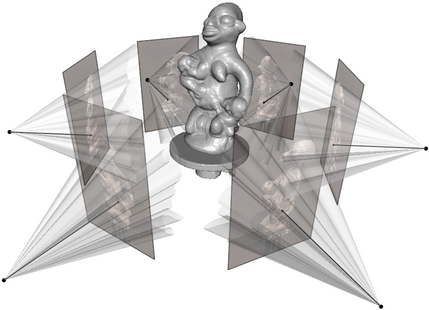
\includegraphics[width=0.2\textwidth]{relatedwork/mvs.png}} &
\raisebox{-0.75\height}{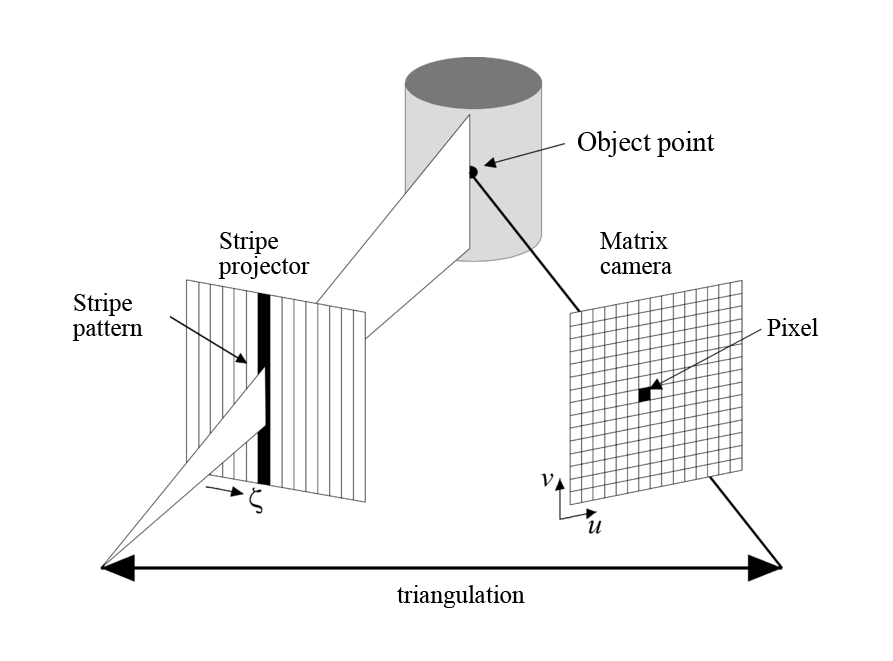
\includegraphics[width=0.2\textwidth]{relatedwork/sl.jpg}} &
Stereo correspondence &
Texture, Albedo, Specular \\
Shape from Intensity & 
\raisebox{-.75\height}{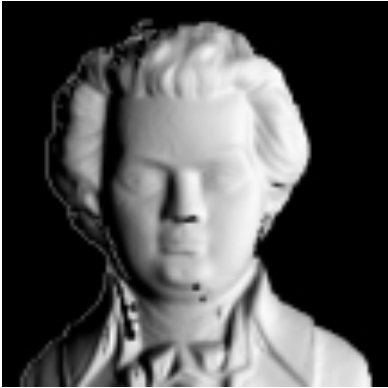
\includegraphics[width=0.15\textwidth]{relatedwork/sfs.png}} &
\raisebox{-.75\height}{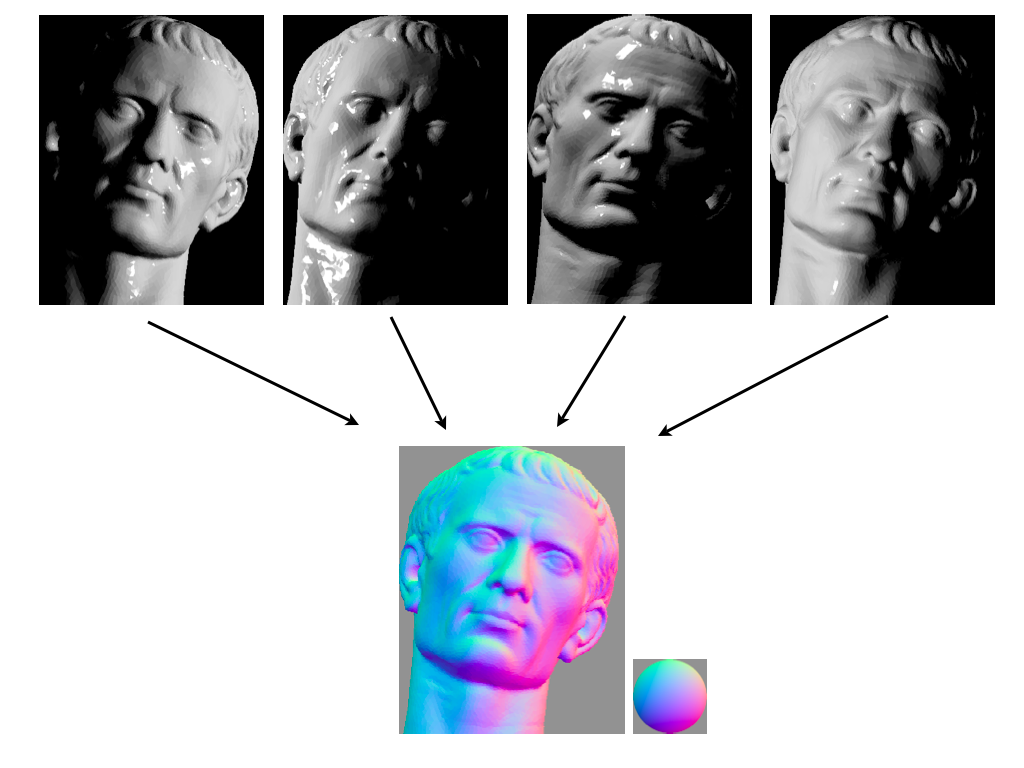
\includegraphics[width=0.2\textwidth]{relatedwork/ps.png}} &
Shading variation &
Albedo, Specular, Geomtry \\
Shape from Silhouette &
\raisebox{-.75\height}{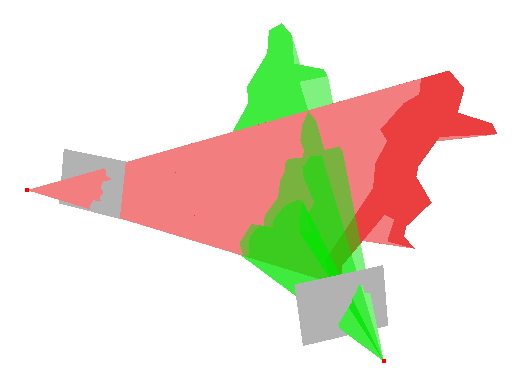
\includegraphics[width=0.2\textwidth]{relatedwork/vh.jpg}} &
\raisebox{-.75\height}{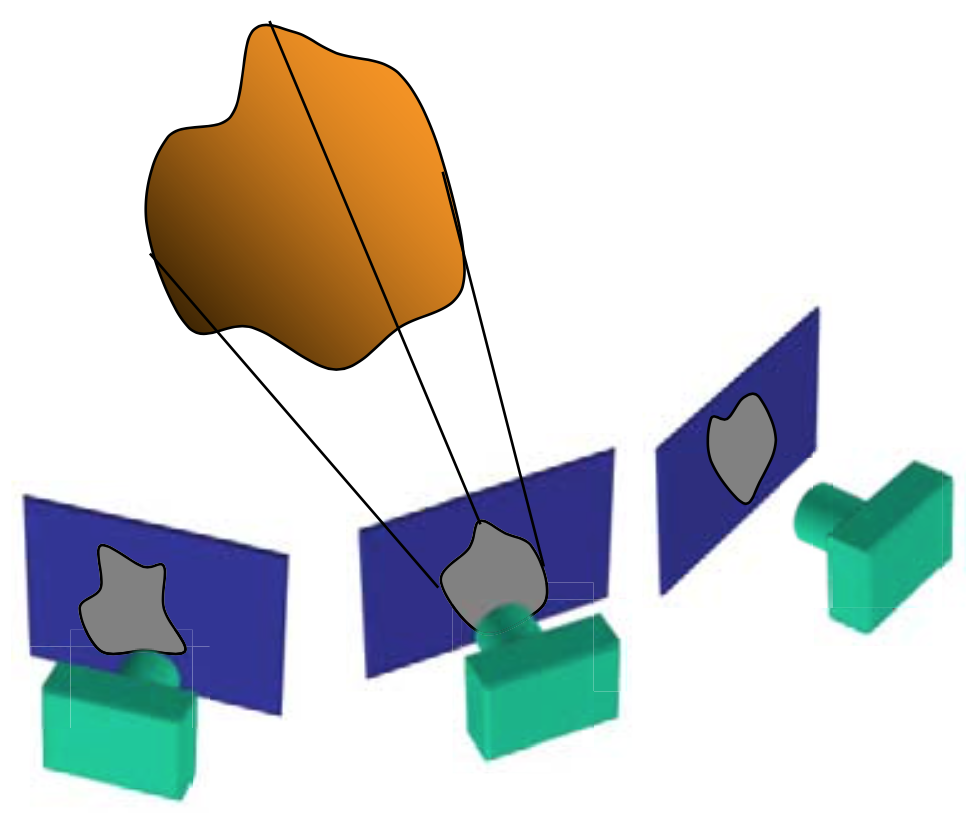
\includegraphics[width=0.2\textwidth]{relatedwork/vh_1.png}} &
Silhouette &
Geoemtry\\
\end{tabular}
\caption{Three classes of algorithms with examples, visual cues used for reconstruction, and potential problems.}
\label{fig:algo_class}
\end{figure}

\subsection{Stereo}
Stereo correspondence is one of the most widely used visual cues in 3D vision. Passive methods, including stereoscopy, trinocular stereo, and MVS, identify correspondences across different views, and estimate the 3D point by triangulation. However these passive approaches suffer from uniform or periodic surfaces. Active techniques attempt to overcome the correspondence problem by replacing one of the cameras with a controllable illumination source, e.g., single-point laser, slit laser scanner, temporal or spatially modulated Structured Light (SL), etc. Here we refer readers to the survey article by \citeauthor{blais2004review} for recent developments of active methods. We classify one of the most widely used passive methods, MVS algorithms, based on the taxonomy proposed in~\cite{seitz2006comparison}, which divides the field into four classes based on reconstruction method, and categorize one of the active methods, Structured Light technique, by projection patterns.

\subsubsection{Passive method: Multi-View Stereo}
\textbf{Volumemetric stereo} algorithms compute a cost function in a 3D volume, then extract a surface from this volume. One successful example is voxel colouring, which traverses a discretized 3D space in “depth-order” to identify voxels that have a unique colouring, constant across all possible interpretations of the scene~\cite{seitz1997photorealistic}. Another thread of work formulates the problem in the Markov Random Field (MRF) framework and extracts the optimal surface by Graph-Cut algorithms~\cite{roy1998maximum,vogiatzis2005multi,vogiatzis2007multiview}.

\textbf{Surface Evolution} algorithms work by iteratively evolving a volume or surface to minimize a cost function. This includes methods based on voxels, level set, and surface meshes. The Space Carving technique achieves a least-commitment shape~\cite{marr1982vision} by iteratively removing inconsistent voxels from the scene~\cite{kutulakos2000theory}. Level-set techniques cast the problem as a variational problem, and use a set of PDE's as cost functions, which are deformed from an initial set of surfaces towards the detected objects~\cite{faugeras2002variational}. Other approaches use a deformable model and represent the scene as surface meshes that moves as a function of internal and external forces~\cite{esteban2004silhouette}. \citeauthor{hiep2009towards} presented a visibility-based method that transforms a dense point cloud into a surface mesh, which is fed into a mesh-based variational refinement that captures small details, smartly handling photo-consistency, regularization and adaptive resolution.

% Level-set based techniques minimize a set of partial differential equations defined in a volume. Like space carving methods, level-set methods typically start from a initial volume and shrink inward, or outward if the cost function is minimized. \citeauthor{faugeras2002variational} proposed a novel geometric approach based on variational principle, from which a set of PDE's can be deduced. The level set method is used to deform an initial set of surfaces towards the objects to be detected. However, level-set is no long a popular MVS technique, because high quailty models with correct topology can be directly computed from photo-consistency functions without the refinement steps.

\textbf{Region Growing} algorithms start with a sparse set of scene points, then propagate these points to spatial neighbours, and refine the cost function with respect to position and orientation of the points. \citeauthor{otto1989region} proposed one of the first work on region growing stereo search~\cite{otto1989region}. The idea of this algorithm is as follows: start with an approximate match between a point in one image and a point in another, use an adaptive least-squares correlation algorithm to produce a more accurate match, and use this to predict approximate matches for points in the neighbourhood of the first match. \citeauthor{lhuillier2002match} proposed a two-view quasi-dense approach, which first sorts a list of point correspondences into a list of seed points by correlation score. Next, at each step of the propagation, a `best' seed point is chosen. Lastly, in the immediate spatial neighborhood of this seed point, new potential matches are checked and the best points are added to the current list of seed points~\cite{lhuillier2002match,lhuillier2005quasi}. This ``best-first'' strategy guarantees convergence by choosing only new matches that have not yet been selected. Further, a patch based approach is proposed that undergoes multiple iterations of matching, propagation, and filtering~\cite{furukawa2010accurate}. A stereoscopic approach called PatchMatch Stereo, which is inspired by an approximate nearest neighbour matching algorithm called PatchMatch~\cite{Barnes:2009:PAR}, starts by randomly assigning an oriented plane to each pixel in two views. Next, each pixel is taken through three iterations of propagations and refinement. The plane is propagated to spatial neighbours, the corresponding pixel from another view, and across time. It can achieve sub-pixel accuracy, but is computationally heavy and challenging for parallelism. There has been some efforts to apply PatchMatch Stereo to multi-view scenarios~\cite{galliani2015massively,uh2014efficient,zheng2014patchmatch}, and develop new propagation schemes to increase the computational efficiency~\cite{galliani2015massively}.
%[has nice math derivations] Shen, Accurate Multiple View 3D Reconstruction Using Patch-Based Stereo for Large-Scale Scenes\\

\textbf{Depthmap Merging} algorithms work by computing a per-view depthmap. By treating a depthmap as a 2D array of 3D points, multiple depthmaps can be considered as a merged 3D point cloud. A `winner-takes-all' approach uses a set of discretized depth values and picks the value with the highest photo-consistency score for each pixel independently. Uniform depth sampling may suffice for simple and compact objects. However, for complex and large scenes, a proper sampling scheme is crucial to achieve high speed and quality. More sophisticated cost functions are derived to account for occlusion or non-Lambertian effects which may add noise to the photo-consistency score~\cite{goesele2006multi,vogiatzis2007multiview}. In the case of severe occlusion, spatial consistency can be enforced under the assumption that neighbouring pixels have similar depth values. This can be formulated under the Markov Random Field (MRF) framework, where the problem becomes minimizing the sum of a unary $\Phi(\cdot)$ and pairwise term $\Psi(\cdot, \cdot)$. The unary term reflects the photo-consistency score of assigning a depth value $d_p$ from a set of depth value to the pixel $p$, whereas the pairwise term enforces the spatial regularization, and assigns the cost of setting depth label $k_p$, $k_q$ to a pair of neighbouring pixels $p$ and $q$, respectively.
$$
E(\{k_p\})= \sum_p \Phi(k_p) + \sum_{(p,q)\in\mathcal{N}}\Psi(k_p, k_q)
$$

MVS algorithms generally have a less strict requirement on the setup, and work relatively reliably in unconstrained envirionments. However, it suffers under the following two conditions:

\textbf{Lack of texture}: Multi-View Stereo algorithms take advantage of textural information to establish point correspondences across different views. Thus homogeneous surfaces pose great challenges to MVS algorithms. We have witnessed surprisingly good results on a textureless object ``Dino'' in the Middlebury MVS benchmark~\cite{seitz2006comparison}. It turns out that MVS algorithms are able to exploit very weak and intricate image textures, most of which come from shading and/or shadowing effects. However, these texture are so weak that images have to have very high quality.

\textbf{Non-Lambertian surface}: MVS algorithms require to observe the same surface patch from different angles in order to establish correspondences across views. Thus, the same surface patch needs to have similar or same appearance from different perspectives, and hence, most of the algorithms assume Lambertian reflectance. Pure Lambertian surfaces are rare in reality, but it is empirically verified that most MVS algorithms perform reasonably well on non-Lambertian surfaces. As long as the cameras can capture the diffuse reflectance component, then the photo-consistency function is able to identify and ignore images whose non-diffsue effects (e.g., specular highlights) are strong, then utilize the diffuse component in the remaining images. Further, there are some attempts to overcome this limitation, a pure passive methods was proposed that directly model and analyze non-Lambertian effects for MVS algorithms~\cite{jin2003multi,jin2005multi}.

\subsubsection{Active method: Structured Light}
To overcome the problem of lack of texture, one of the cameras in stereoscopy can be replaced by an illumination source, \eg a projector, which is called Structured Light technique. It is based on projecting a temporally or spatially modulated pattern onto a surface and viewing the illuminated surface from one or more points of view. The correspondence is easily detected from the projected and imaged pattern, which is triangulated to obtain the a 3D point. Each pixel in the pattern is assigned a unique codeword, and the codeword is encoded by using grey level, colour or geometric representations. Structured Light is classified based on the following coding strategy: temporal, spatial and direct codification~\cite{salvi2004pattern}. Temporal techniques generate the codeword by projecting a sequence of patterns. Spatial codification represents each codeword in a unique spatial pattern. Direct codification techniques define a codeword for every pixel, which is equal to its grey level or colour.

\textbf{Temporally encoded} SL projects a sequence of patterns successively onto the surface. The codeword for a given pixel is formed by a sequence of illuminaiton values for that pixel across the projected patterns. This kind of pattern can achieve high accuracy due to two factors: 1) the codeword basis is small (e.g., two for binary pattern), therefore, each bit is easily distinguishable; 2) a coarse-to-fine strategy is used, and the position of the pixel becomes more precise as the patterns are successively projected. This technique can be further classified by the way pattern is encoded temporally: 1) binary codeword; 2) $n$-ary codeword; 3) gray code combined with phase shifting; 4) hybrid techniques. More details are available in this review~\cite{salvi2004pattern}.

\textbf{Spatially encoded} techniques concentrate all coding into a unique pattern. The codeword that labels a certain pixel is obtained from the neighbourhood of pixels around it. Normally, the visual features gathered in a neighbourhood are the intensity or colour of the pixels or groups of pixels around it.

\textbf{Directly encoded} methods represent the codeword in each pixel directly. To achieve this, we need to use either a large range of colour values or introduce periodicity. However, this kind of pattern is highly sensitive to noise because the ``distance'' between codewords is nearly zero. Moreover, the perceived colour depends not only on the projected colour, but also the intrinsic colour of the surface. Therefore, reference images must be taken to eliminate the effect of surface colour. This kind of coding can be further classified as: 1). codification based on grey levels; 2). codification based on colour. More details are available in review~\cite{salvi2004pattern}.

Structurd Light techniques overcomes the lack of texture problem by actively projecting a pattern onto the surface. However, it still suffers under the following conditions:

\textbf{Low surface albedo} poses a great challenge to active methods, such as SL, which utilize reflected light to establish correspondences across different views. Regardless of which projection pattern is used, the most critical component of any SL system is the decoding process, which retrieves per-pixel codeword from the imaged projection pattern. Thus, the surface albedo needs to be strong enough so that sufficient amount of reflected light can reach the camera sensor.

\textbf{Non-Lambertian surfaces} exhibit strong reflection in the specular direction. Images of such surfaces are challenging to interpret due to the bright points or highlights, which makes the projected pattern indistinguishable in these areas. Thus, it is impossible to decode the pixels exhibiting specular effects.

\textbf{Concavity} is the cause of global light transport, such as inter-reflection, which results in surface patches receiving light from sources other than the projector. Thus, the intensity value or colour of a pixel becomes noisier, which seriously affects the accuracy of decoding process.

\subsection{Shading}
Shading variation is an effective visual cue for retrieving shape of a surface. Shading variation depends on surface geometry (surface orientation), reflectance (material), and lighting (illumination). This is generally an ill-posed problem because different shapes illuminated under different light conditions may produce the same image. It becomes possible to estimate surface orientation once the reflectance property and illumination are known. This technique of estimating surface shape by shading variation is called Shape from Shading. However, this technique requires strict constraints on surface geometry since only one input image is used, which leads to a novel technique called Photometric Stereo in which surface orientation is determined from two or more images. The idea of Photometric Stereo is to vary the direction of the incident illumination between successive views while holding the viewing direction constant. This provides enough information to determine surface orientation at each pixel~\cite{woodham1979photometric}. This technique can produce a surface normal map with the same resolution of the input image, \ie to produce the pixel-wise surface normal map. Since the coefficients of the normal map are continuous, the integrated height map can reach an accuracy that cannot be achieved by any triangulation methods. Therefore, the Photometric Stereo technique is more desirable if the intrinsic geometric details are of great importance.

\subsubsection{Shape from Shading}
The problem of recovering the shape of a surface from intensity variation is first proposed by Horn~\cite{horn1970shape}. It assumes that the surface under consideration is of a uniform albedo and reflectance, and that the direction of the single distant light source is either known or can be calibrated by the use of a reference object. Thus the intensity $I(x,y)$ becomes purely a function of the local surface orientation. The information of reflectance, illumination, and viewing geometry can be combined into a single function called reflectance map $R(p, q)$, that relates surface orientation directly to image intensities:
\begin{align*}
I(x, y) &= R(p(x, y), q(x, y))
% I(x, y) &= \rho(\vec{n},\vec{l})\vec{n}^\top\vec{l} \quad (\text{Lambertian model})
\end{align*}
where $(p, q) = (z_x, z_y)$ are surface gradients. Unfortunately, there are more unknown (per-pixel gradient) than there are measurements (per-pixel intensity). More specifically, surface orientation has two unknowns($p, q$) whereas measurements of the brightness at a single pixel only provide one constraint. Thus, additional information regarding the surface reflectance and illumination, as well as constraints on surface geometry, such as smoothness or integrability are required to estimate $(p, q)$. One common used constraint is smoothness:
\begin{align*}
\int p_x^2 + p_y^2 + q_x^2 + q_y^2 \mathrm{d}x\mathrm{d}y = \int \|\nabla p\|^2+\|\nabla q\|^2 \mathrm{d}x\mathrm{d}y
\end{align*}
Another is the integrability constraint:
\begin{align*}
\int(p_y-q_x)^2 \mathrm{d}x\mathrm{d}y
\end{align*}
since for a valid depth $z(x, y)$ with $(p, q)=(z_x, z_y)$, we have $p_y=z_{xy}=z_{yx}=q_x$.

% The Shape from Shading problem is an ill-posed problem since it need to solves for two unknown (surface normal, gradient) with only one input (per-pixel intensity). With additional constraints regarding the surface smoothness, this problem can potentially be solvable.

Most shape from shading algorithms assume that the surface under consideration is of a uniform albedo and reflectance, and that the light source directions are either known or can be calibrated by the use of a reference object. Thus, they are applicable to textureless surfaces with uniform and known albedo. Besides, a tedious calibration step needs to be carried out to estimate light direction and intensity. However, even by assuming the simplest reflectance model, Lambertian reflectance, the survey by Zhang~\cite{zhang1999shape} demonstrated that SfS algorithms generally perform poorly, and none performs well in all cases.

% \textbf{Texture: textureless}
% Typical SfS algorithms asssume surfaces with uniform and known albedo, \ie textureless surfaces.

% \textbf{Brightness}
% Active methods such as SfS utilize reflected light to estimate surface depth or orientation information. In this case, the intensity variation is used to estimate surface normal, thus the surface should have sufficiently high albedo, otherwise, the intensity variation would be hard to detect.

% \textbf{Reflectance}
% Though other reflectance models are feasible, typical SfS algorithms assume Lambertian reflectance model. The reason is that surface lightness is directly related to surface orietation and reflectance model once the light source and viewing direction are fixed. This is generally an ill-posed problem even with Lambertian model since there is only one intensity value per pixel to solve for surface orientation, which has two DoF. 

% \textbf{Concavity}
% Typical SfS algorithms can not deal with effects caused by global light transport, such as cast shadow, inter-reflection, and so on. The surface lightness would be corrupted by light transported from other surface facets. Thus, objects exhibit any form of concavity will pose great challenge to SfS algorithms.

\subsubsection{Photometric Stereo}
The \textbf{Classical Photometric Stereo}, first proposed by Woodham~\cite{woodham1980photometric}, utilized multiple light sources from different directions to overcome the ambiguity of Shape from Shading. Assuming Lambertian reflectance, $P$ pixels per image, and $Q$ illumination directions, the intensity of the $i$th pixel under $j$th illumination is
\begin{align*}
I_{i,j} &= \rho_i\vec{n}_i^\top \vec{l}_j\\
\Rightarrow\mathbf{I} &= \mathbf{N}^\top \mathbf{L}
\end{align*}
where $\mathbf{I}\in \mathbb{R}^{P\times Q}$ stores the pixel intensity from all images. Each column contains pixels from each image while each rows contains intensity of each pixel under all illumination conditions. $\mathbf{N}\in \mathbb{R}^{P\times3}$ encodes the albedo-scaled surface normal for each pixel, \ie $N_{i, :} = \rho_i\vec{n}_i^\top$. $\mathbf{L} \in \mathbb{R}^{3\times Q}$ encodes the light source directions, \ie $L_{:, j} = \vec{l_j}$. This surface reflectance, \ie spatially varying albedo $\rho_i$, and the normal $n_i$ can be estimated by
\begin{align*}
\mathbf{N} &= \mathbf{I}\mathbf{L}^{+}\\
\Rightarrow\rho_i &= \|\mathbf{N}_{i,:}\|\\
\Rightarrow n_i &= \frac{\mathbf{N}_{i,:}^\top}{\|\mathbf{N}_{i,:}\|}
\end{align*}

Thus, the problem of estimating shape of a Lambertian surface under known lighting conditions has a simple solution. However, this algorithm fails to work once these constraints are violated. Thus, past research efforts have been focused on generalizing various assumptions made by classical photometric stereo. For the camera assumption, orthographic projection can be achieved by using a lens with long focus and placing the objects far from the camera. The nonlinear response can be solved by performing radiometric calibration. The shadow and other global light transportation are a few of the sources of errors, where some approaches consider them as outliers and remove them before normal estimation. The reflectance and lighting assumptions, however, are the most complicated since the reflectance properties depends on material property and microscopic structure. Further, lighting can have either an arbitrary or fixed position, orientation, and intensity. Therefore, research on Photometric Stereo are generally on two directions: 1) generalization of reflectance; 2) generalization of lighting conditions. A summary of assumptions made by various classes of PS algorithms are presented in Table~\ref{tab:ps_assumptions}.
\begin{table}[!htbp]
  \centering
  \begin{tabular}{p{2cm}|cp{4cm}c}
  \toprule
  \textbf{Category} & Camera & Light source & Reflectance \\
  \midrule
  Classical PS & Orthographic & Directional, known intensity and direction & Lambertian \\
  Generalized lighting PS & Orthographic & Unknown intensity and direction, ambient & Lambertian \\
  Generalized reflectance PS & Orthographic & Distant, known intensity and direction & Non-Lambertian \\
  \bottomrule
  \end{tabular}
  \caption{Assumptions made by different classes of photometric stereo.}
  \label{tab:ps_assumptions}
\end{table}

\textbf{Generalization of Lighting} 
It is possible to estimate the surface orientation without knowing light directions, a case also known as \textit{uncalibrated Photometric Stereo}, see Table~\ref{tab:ps_assumptions}. Most uncalibrated techniques assume Lambertian techniques and are based on factorization technique proposed in \cite{hayakawa1994photometric}. Recall the irradiance equation:
$$
\mathbf{I}=\mathbf{N}^\top \mathbf{L}
$$
However, an infinite number of candidates $\hat{N}$ and $\hat{L}$ make the above equality met. In fact, any invertible $3\times 3$ matrix $G$ defines a candidate pair $\hat{N} = N\cdot G, \hat{L}=G^{-1}L$. Thus the normal $N$ and light source direction $L$ can only be recovered up to a linear transformation. It has been shown that only a 3-parameter subset of these transformations, known as the Generalized Bas-Relief (GBR) ambiguity, preserve surface integrability~\cite{belhumeur1999bas}.

Other generalized lighting conditions are any situations other than the ideal case of using a single distant point light source in a dark room, such as natural ambient light, multiple point light sources with/without ambient lighting, etc. To make the problem more tractable, the reflectance model should no longer be a general one, as this involves too many degrees of freedom that results in many different shapes with incorrectly estimated general reflectance and incorrectly estimated general lighting.

\textbf{Generalization of Reflectance} This direction of research has been to relax the assumption of Lambertian reflectance. This can be broadly divided into four classes of algorithms.

\textit{Outlier rejection} approach assumes that Non-Lambertian reflectance can be well approximated by the sum of diffuse and specular lobe. The specular pixels are considered as outliers in ~\cite{coleman1982obtaining} and \cite{barsky20034}. Others assume that the color of the specular lobe differs from that of the diffuse lobe, which allows the separation of the specular and diffuse components~\cite{mallick2005beyond,sato1994temporal,schluns1993photometric}.

\textit{Reference object} approach uses a reference object that has similar material as the target object. This is proposed in~\cite{silver1980determining} and later revisited in~\cite{hertzmann2005example}. The idea is that surface points with same orientation give similar intensity values under similar reflectance and lighting. It can deal with arbitrary BRDFs as long as the reference and target object has the same material. It can handle spatially-varying BRDFs as long as there are multiple reference objects. Each reference object serves as a ``basis'' BRDF, and the BRDF at any point on the target object can be approximated as a linear combination of the basis BRDFs.

\textit{Parametric reflectance model} approach builds upon the idea that an arbitrary BRDF can be approximated by ``basis'' BRDFs, and replaces the reference objects with sophisticated BRDF models. An isotropic Ward model is used as basis BRDF, and the surface orientation and parameters of the reflectance models are estimated iteratively~\cite{goldman2010shape}.

\textit{Invariants of BRDF} approach exploits various physical properties of BRDFs. While parametric reflectance models are very good at reducing the complexity of BRDFs, they are usually only valid for a limited class of materials. An alternative is to exploit the invariants of BRDFs, typically including energy conservation, non-negativity, Helmholtz reciprocity, isotropy, and so on~\cite{zickler2002helmholtz,alldrin2007toward}.

Photometric Stereo can work extremly well under certain constrained conditions. However, it generally performs poorly once the aforementioned assumptions are violated: the classical PS and generalized reflectance PS fail to work under uncalibrated light conditions. The generalized lighting PS only handle Lambertian surfaces under uncalibrated lighting conditions, but only achieves estimation up to a linear transformation; the classical PS and generalized lighting PS fail to work under generalized reflectance conditions; and lastly, most PS algorithms fail to work on conditions of generalized lighting and reflectance, one approach that has been proved to work is to place multiple reference objects in the scene with the target object as proposed by~\cite{hertzmann2005example}.

% \subsubsection{Limits: PS}
% \textbf{Texture} 
% Though SfS algorithms require uniform and known albedo, typical PS algorithms can be used easily on surfaces with spatially varying albedo. For instance, the albedo-scaled normal can be estimated, then the albedo is retrieved as the magnitude of the scaled normal~\cite{woodham1980photometric}.

% \textbf{Brightness} 
% Active methods such as PS utilize reflected light to estimate surface depth or orientation information. In this case, PS algorithms work more reliably on surfaces with sufficiently strong albedo. This is because the algorithm exploits the intensity variation as a visual cue, which is more challenging to detect on surfaces with low intensity values.

% \textbf{Reflectance} % Lambertian PS: uniform reflectance
% The Lambertian PS algorithms can be divided into two groups: calibrated, and uncalibrated method. The classical PS proposed by Woodham~\cite{woodham1980photometric} can be considered as calibrated Lambertian PS. Later, more uncalibrated Lambertian PS algorithms have been proposed to avoid this tedious process.

% \textbf{Convexity} 
% Active methods that assumes a \textbf{local interaction model}, such as most PS algorithms, can work more reliably on surfaces without casting shadow and inter-reflection. Thus surfaces with concavities pose a great challenge for this type of techniques since the indensity can be affected by other surface patches.

% [Some other papers to read] \\
% - R. J. Woodham. Photometric method for determining sur-
% face orientation from multiple images.\\
% 1. joint recovery of unknown shape and reflectance\\
% - N. Alldrin, T. Zickler, and D. Kriegman. Photometric stereo with non-parametric and spatially-varying reflectance.\\
% - D. Goldman, B. Curless, A. Hertzmann, and S. Seitz. Shape and spatially-varying BRDFs from photometric stereo.\\
% - T. Higo, Y. Matsushita, and K. Ikeuchi. Consensus photometric stereo.\\
% - B.Shi,P.Tan,Y.Matsushita,and K.Ikeuchi. Elevationangle from reflectance monotonicity: Photometric stereo for general isotropic reflectances.\\
% - BOXIN SHI's PhD thesis\\
% - Satoshi Ikehata's PhD thesis\\
% 2. a less restrained capture setup with arbitrary and unknown illumination\\
% - H. Hayakawa. Photometric stereo under a light source with arbitrary motion\\
% - T. Papadhimitri and P. Favaro. A new perspective on uncalibrated photometric stereo\\
% - B. Shi, Y. Matsushita, Y. Wei, C. Xu, and P. Tan. Self-calibrating photometric stereo\\
% 3. combine both directions\\
% - A.Hertzmannand S.Seitz.Shapeandmaterialsbyexample: a photometric stereo approach.\\
% - A. Hertzmann and S. Seitz. Example-based photometric stereo: shape reconstruction with general, varying BRDFs.\\
% - W. M. Silver. Determining shape and reflectance using mul- tiple images. Master’s thesis, MIT, 1980.\\

\subsection{Silhouette}
In some cases, it's an easy task to perform a foreground segmentation of the object of interest, which leads to a class of techniques that reconstructs a 3D volumetric model from the intersection of the binary silhouettes projected into 3D. The resulting model is called a \textit{visual hull}.

The basic idea of shape from silhouette algorithms is that the object lies inside the intersection of all visual cones back-projected from silhouettes. Suppose there are multiple views $V$ of the target object. From each viewpoint $v\in V$, the silhouette $s_v$ can be extracted, which is the region including the object's interior pixels and delimited by the line(s) separating the object from the background. The silhouette $s_v$ are generally non-convex and can represent holes due to the geometry of the object. A cone-like volume $cone_v$ called (truncated) extended silhouette is generated by all the rays starting at the center of projection and passing through all the points of the silhouette. The target object is definitely internal to $cone_v$ and this is true fro every view $v'\in V$; it follows that the object is contained inside the volume $c_V=\cap_{v\in V}c_v$. As the size of the $V$ goes to infinity, and all possible views are included, $c_V$ converges to a shape known as the \textit{visual hull} $vh$ of the target object.

% Some approaches first approximate each silhouette with a polygonal representation and then intersect the resulting faceted conical regions in 3D space to produce polyhedral models, which can be later refined using triangular splines. Other approaches use voxel-based representations, usually encoded as octrees, because of the resulting time-space efficiency.

[computational complexity] intersection of many volumes can be slow. Simple polyhedron-polyhedron intersection algorithms are inefficient. To improve performance, most methods 1) quantize volumes, 2) perform intersection computation in 2D instead of 3D.

\textbf {Voxel based methods} 
First the object space is split up into a 3D grid of voxels; each voxel is intersected with each silhouette volume; only voxels that lie inside all silhouette volumes remain part of the final shape.

\textbf{Marching intersections based methods} 
The marching intersection (MI) structure consists of 3 orthogonal sets of rays, parallel to the $X$, $Y$, and $Z$ axis, which are arranged in 2D regular arrays, called the $X-rayset$, $Y-rayset$, $Z-rayset$ respectively. Each ray in each rayset is projected to the image plane to find the intersections with the silhouette. These intersections are un-projected to compute the 3D intersection between the ray and the extended silhouette on this ray. This process is repeated for each silhouette, and the un-projected intersections on the same ray are merged by the boolean AND operation.

Once the MI data structure representing the intersection of all extended silhouettes, a triangular mesh is extrated from it. This is done by the MI technique proposed in~\cite{rocchini2001marching} which traverses the ``virtual cells'' implicitly defined by the MI, builds a proper marching cube (MC) entry for them that in turn is used to index a MC's lookup table.

\textbf{Exact polyhedral methods} 
The silhouette is converted into a set of convex or non-convex 2D polygons with holes allowed. The resulting visual hull with respect to those polygonal silouettes is a polyhedron. The faces of this polyhedron lie on the faces of the original cones. The faces of the original cones are defined by the center of projections and the edges in the input silhouettes. The idea of this method is: for each input silhouette $s_i$ we compute the face of the cone. Then we intersect this face with cones of all other input silhouettes, \ie a polygon-polyhedron intersection. The result of these intersections is a set of polygons that define the surface of the visual hull.

% \subsection{Image based method}
% \begin{itemize}
% \item this algorithm will only produce renderings of a visual hull from any view
% \item every pixel in the desired output image is back-projected to form a 3D ray
% \item each of those rays is intersected with each of the input silhouettes in the same way as the rays in the marching intersections method
% \item a pixel in the output image is inside the new rendering of the visual hull if its ray has any segments left in it that are intersecting the visual hull. The depth of these pixels is known from the depth of the nearest entry point on the ray.
% \end{itemize}

Visual Hull algorithms don't rely on material properties as long as the foreground of the image can be reliably segmented, thus is applicable for objects with arbitrary reflectance properties. However, it fails to carve the concavities on the object surface, thus is unsuitable for concave objects.

% All of the cues above are most widely used ones, and achieved decent results. These following two cues haven't resulted in as much success. Therefore, we only discuss the general idea rather than the technical details.

% \subsection{Texture}
% The basic principle behind shape from texture is the \textit{distortion} of the individual texel. In general, the image formation process introduces three distortion effects: the \textit{distance effect}, which makes objects in view appear larger when they are closer to the image plane; the \textit{position effect} which makes objects appear differently when the angle between the line of sight and the image plane different; and the \textit{forshortening effect}, which distort the objects depending on the angle between the surface normal and the line of sight. Besides, different effects take place under different projection models: the orthographic projection captures only the foreshortending effect whereas the perspective projection captures all three. Therefore, shape from texture methods which use orthographic projection are valid only in a limited domain, where the other two effects can be ignored, and the perspective model captures all three effects, but the resulting algorithms are complicated and involves the solution of nonlinear equations.
% \begin{figure}[h]
% \centering
% 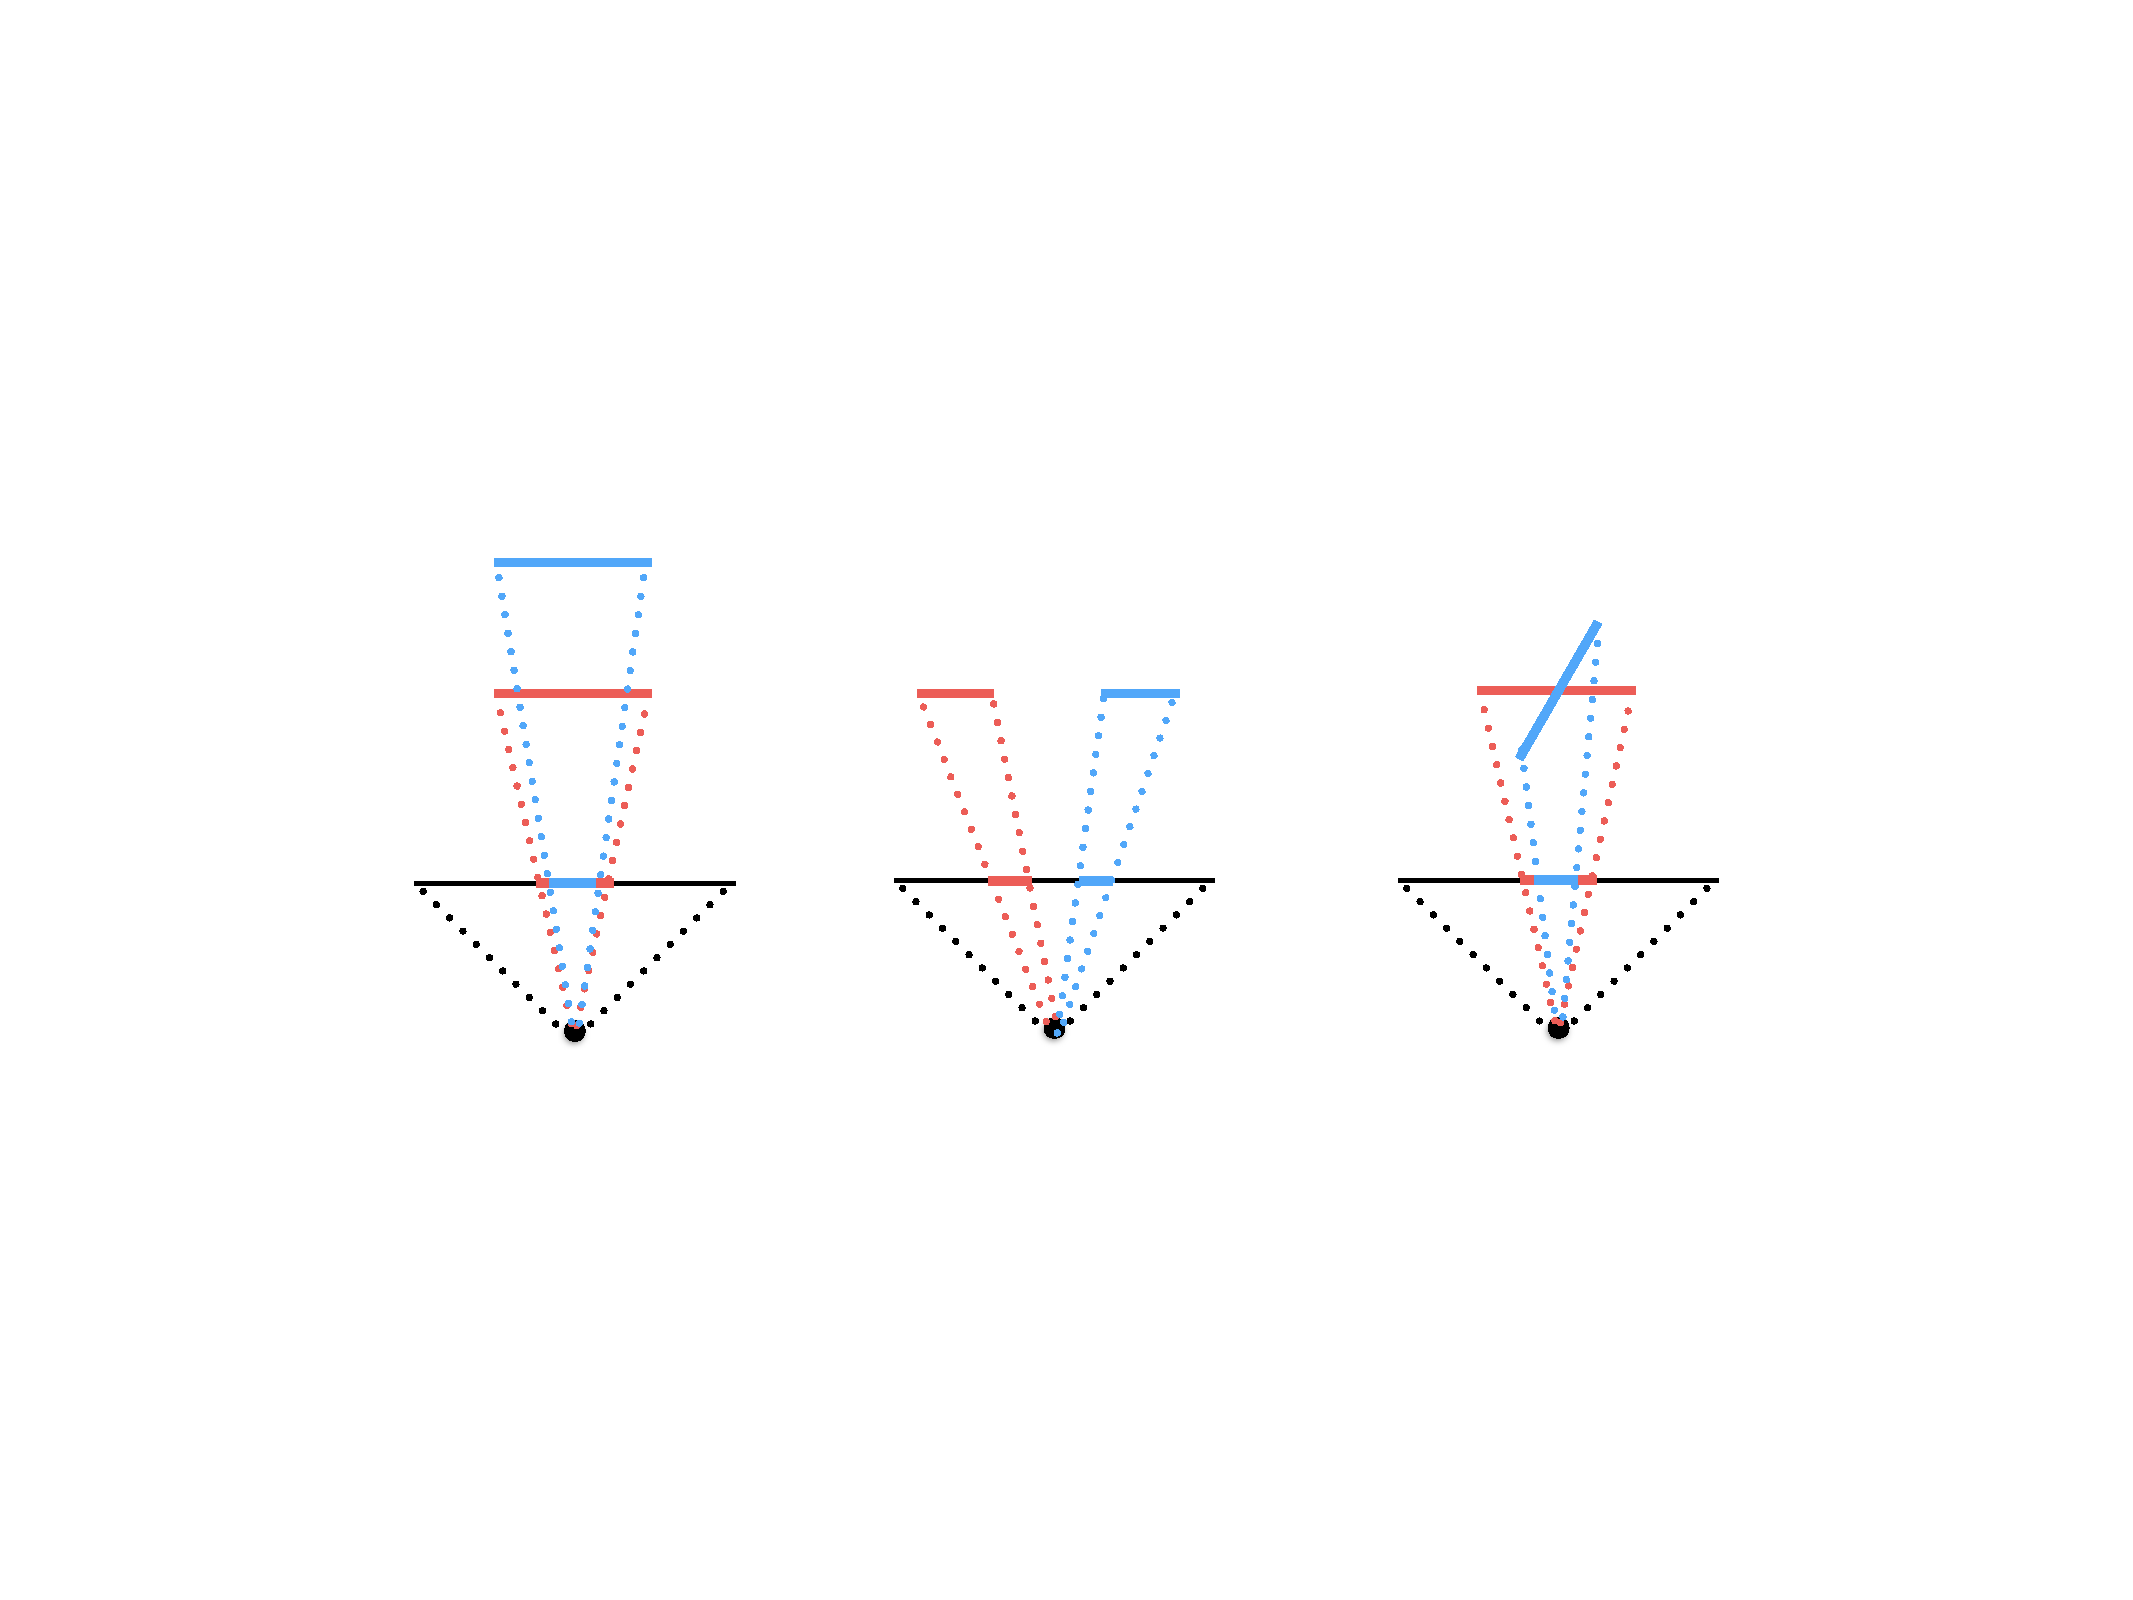
\includegraphics[width=0.8\textwidth]{relatedwork/tex_dist}
% \caption{Three distortion effect: distance distortion, position distortion, and foreshortening distortion.}
% \label{fig:tex_dist}
% \end{figure}

% To calculate the surface curvature at any point is far from trivial. Therefore, the surface shape is reconstructed by calculating the surface orientation (surface normal). A map of surface normals specifies the surface's orientation only at the points where the normals are computed. But, assuming that the normals are dense enough and the surface is smooth, the map can be used to reconstruct the surface shape.

% \subsection{Defocus}
% \textbf{Shape from focus}
% A strong cue for object depth is the amount of blur, which increases as the object moves away from the camera's focusing distance. As shown in Figure~\ref{fig:thin_lens}, moving the object surface away from the focus plane increases the circle of confusion.

% \begin{figure}[h]
% \centering
% 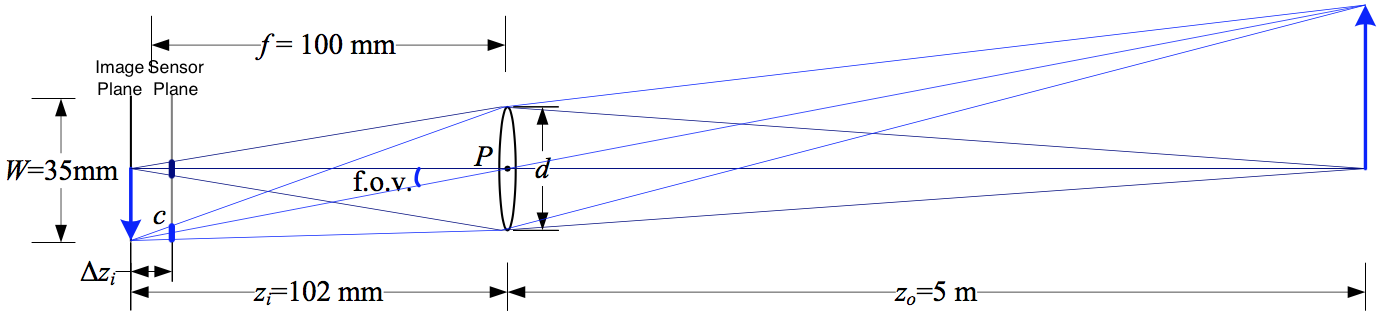
\includegraphics[width=0.8\textwidth]{relatedwork/thin_lens}
% \caption{A thin lens of focal length $f$ focuses the light from a plane a distance $z_0$ in front of the lens at a distance $z_i$ behind the lens, where $\frac{1}{z_o}+\frac{1}{z_i}=\frac{1}{f}$. If the sensor plane moved forward $\Delta z_i$, the image are no longer in focus and the \textit{circle of confusion} $c$ depends on the distance of the sensor plane motion $\Delta z_i$ relative to the lens aperture diameter $d$.}
% \label{fig:thin_lens}
% \end{figure}

% Figure~\ref{fig:thin_lens} shows the basic geometric image formation. The relationship between the object distance $z_o$, focal distance of the lens $f$, and the image distance $z_i$, is given by the Gaussian lens law:
% $$
% \frac{1}{z_o}+\frac{1}{z_i}=\frac{1}{f}
% $$
% All light rays that are radiated from the object and intercepted by the lens to converge at a single point on the image plane, thus a \textit{focused} image $I_f(x, y)$ is formed on the image plane. If, however, the sensor plane does not coincide with the image plane and is displaced from the image plane by a distance $\Delta z_i$, the energy received from the object is uniformly distributed over a circular patch on the sensor plane. The relationship between the radius $c$ of the circle of confusion and the sensor displacement $\Delta z_i$ is as follows:
% $$
% c = \frac{\Delta z_i r}{z_i}
% $$
% where $r$ is the radius of the lens. If we assume that the radius $c$ of the circle of confusion is independent of the position of the object point. Therefore, the \textit{defocused} image $I_d(x, y)$ formed on the sensor plane can also be obtained by convolving the focused image $I_f(x, y)$ with a circular symmetric ``pillbox'' filter
% $$
% I_d(x, y)=p(x, y)*I_f(x, y)
% $$
% where
% $$
% p(x, y) = \begin{cases}
%     \frac{1}{\pi r^2}       & \quad \text{if } x^2+y^2\leq r^2\\
%     0  & \quad \text{otherwise}\\
%   \end{cases}
% $$
% The defocused images can be obtained in three ways: by displacing the sensor with respect to the image plane, by moving the lens, or by moving the object with respect to the object plane. The first two ways cab cause the following problems:
% \begin{itemize}
% \item The magnification of the system varies, thereby causing the image coordinates of the object points to change.
% \item The area on the sensor plane over which light energy is distributed varies, thereby causing a variation in image brightness.
% \end{itemize}
% To address this issue, the degree of focus is changed by moving the object with respect to a fixed configuration of the optical system and sensor. This approach ensures that the focused areas of the image are always subjected to the same magnification.

% The idea is as follows: the stage is moved in increaments of $\Delta d$, and an image is captured at each stage position ($d=n\Delta d$). By studying the behaviour of the focus measure, an interpolation method is used to compute the accurate depth estimates from a small number of focus measures. An important feature of this method is the local nature, the depth estimate at an image point is computed only from focus measures recorded at that point.
% \begin{figure}[h]
% \centering
% 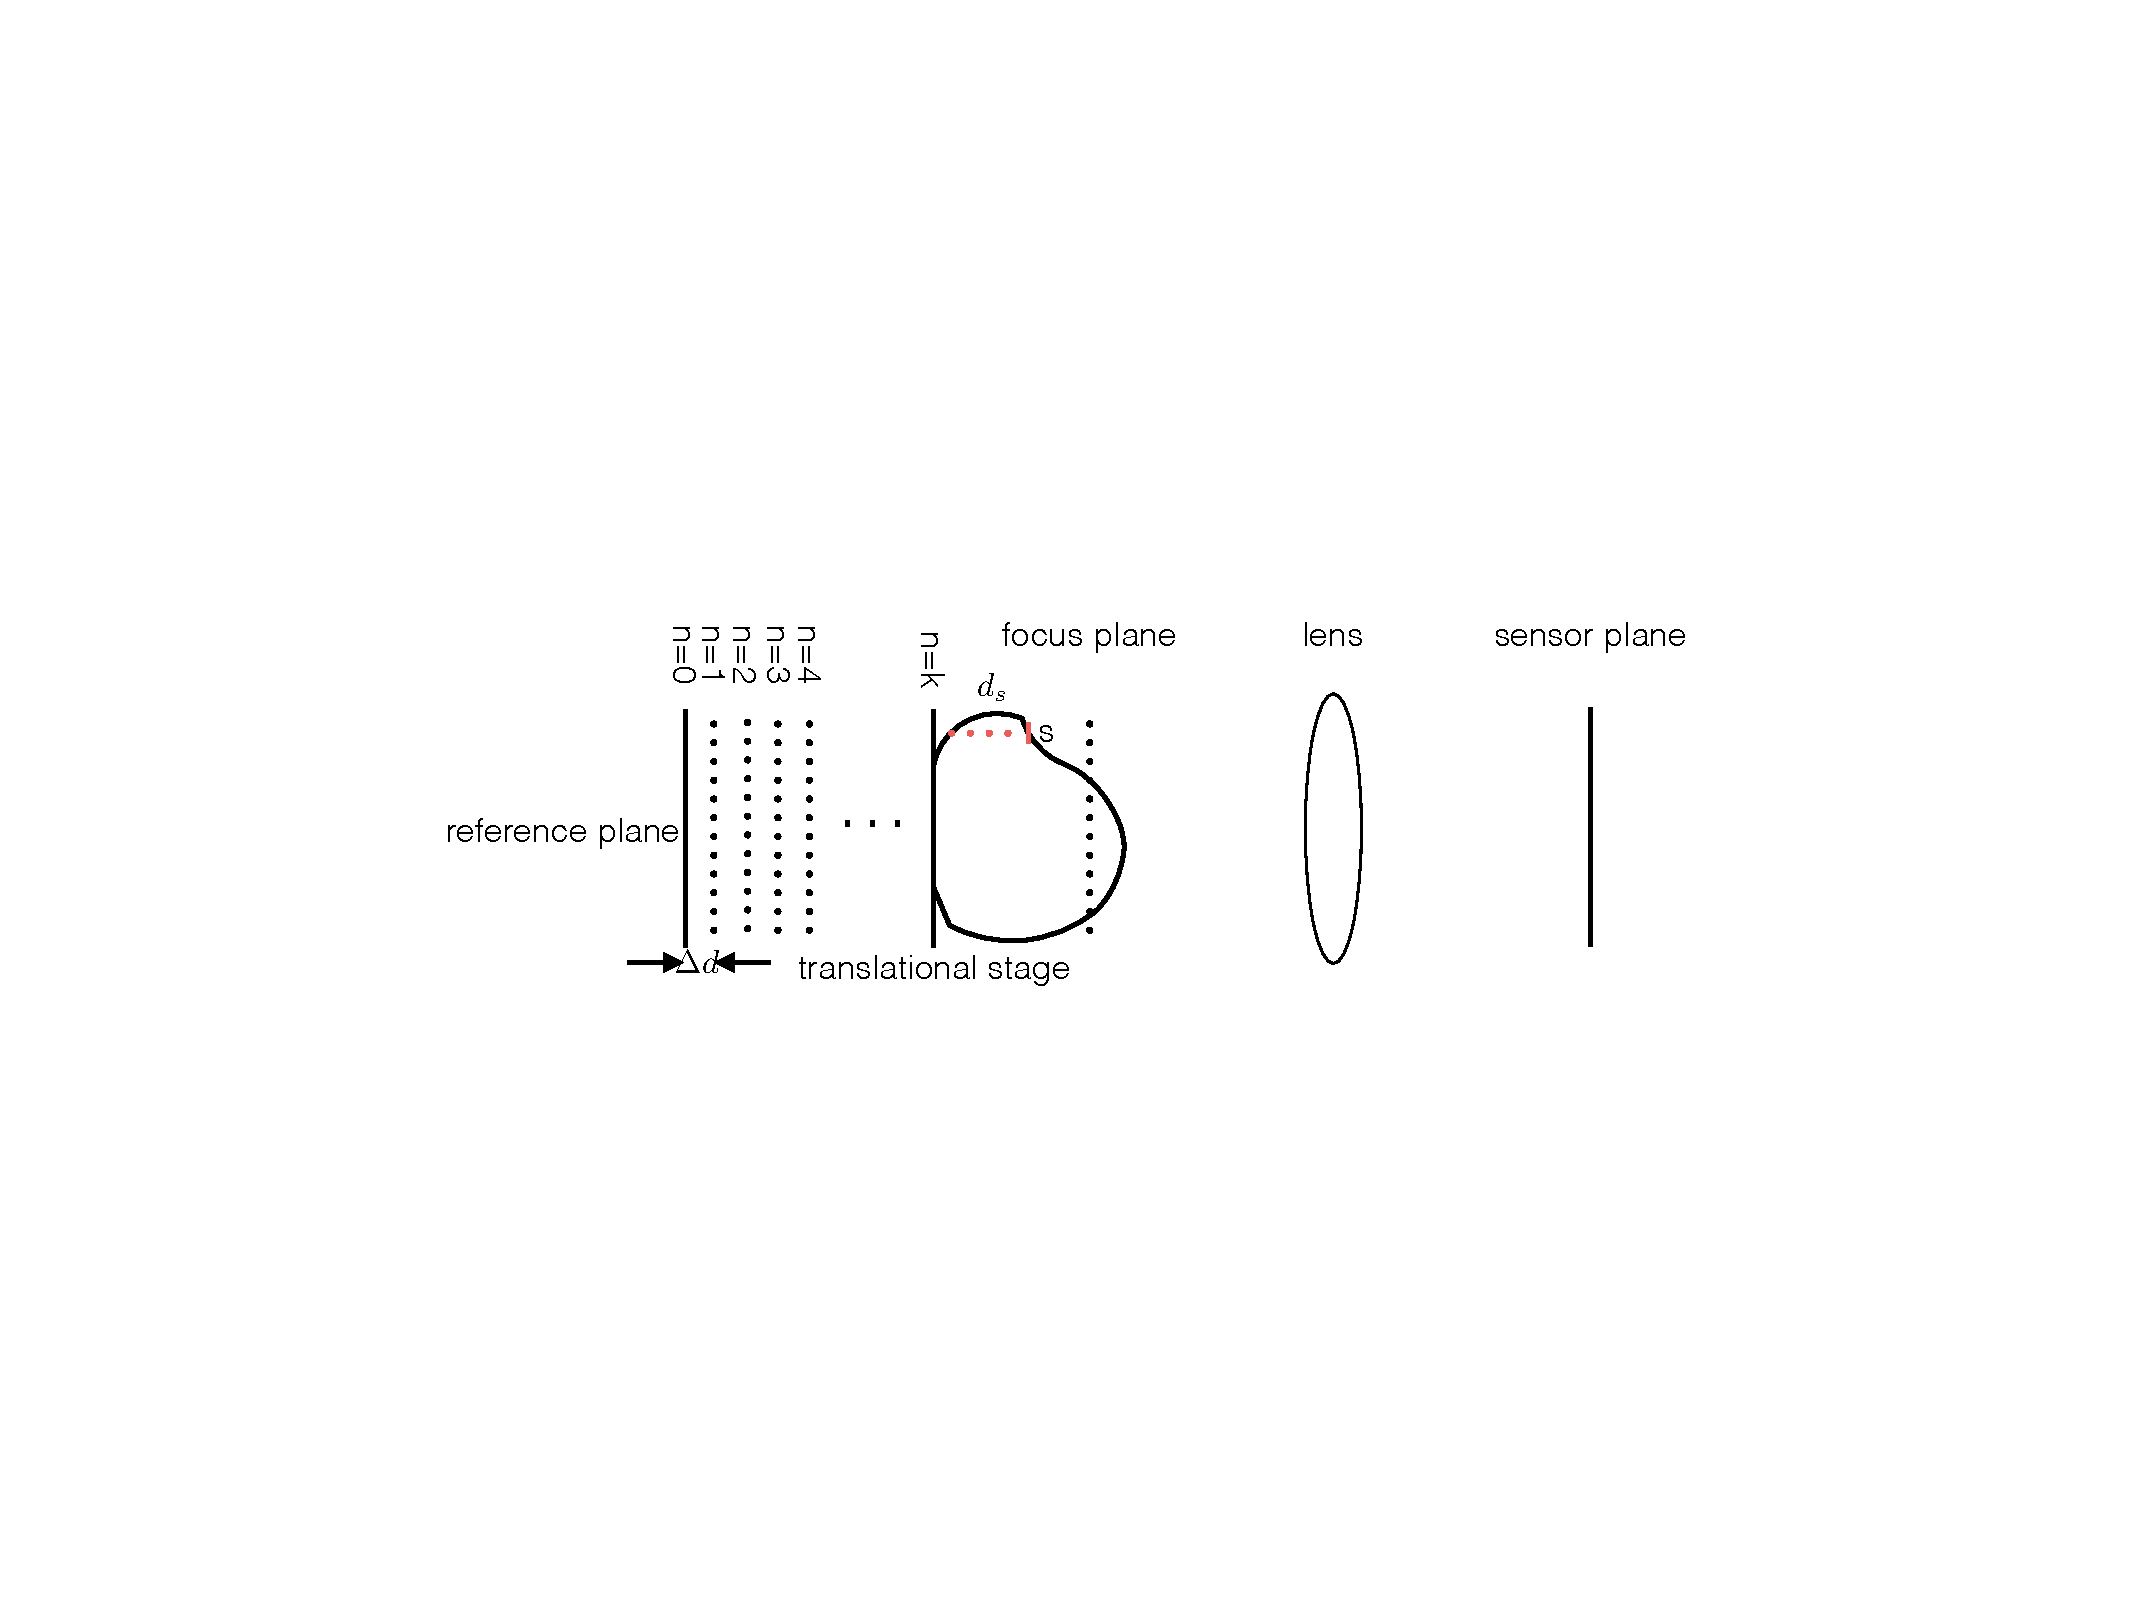
\includegraphics[width=0.8\textwidth]{relatedwork/shape_from_focus}
% \caption{shape from focus}
% \label{fig:shape_from_focus}
% \end{figure}

% \include{paper}
%% The following is a directive for TeXShop to indicate the main file
%%!TEX root = diss.tex

\chapter{A Taxonomy of 3D Reconstruction}
\label{ch:3DRecon_Taxo}
Existing taxonomies of 3D reconstruction techniques generally focus on one category of techniques: \citeauthor{seitz2006comparison} proposed taxonomy of Multi-view Stereo algorithms from various perspectives of algorithmic details. Reviews of Structured Light techniques typically classify techniques based on the type of projection pattern used~\cite{geng2011structured, salvi2004pattern}. Photometric Stereo algorithms are classified by the assumptions or generalizations made, such as, unknown/known reflectance, unknown/known light conditions (uncalibrated/calibrated), and so on~\cite{shi2016benchmark}. These frameworks provide a way to categorize intra-category algorithms, but are unsuitable to evaluate the performance of inter-category algorithms. Furthermore, the algorithms under consideration target limited categories of objects. It is well known that such algorithms are highly likely to fail when targeting a diverse set of object categories. Thus, it is crucial to understand where algorithms perform well and where they fail when designing an application for reconstruction. Under the previous framework of taxonomy, this knowledge is largely empirical, with each algorithm mapped roughly to a sub-volume in the problem space that is poorly defined. To overcome this limitation, we need to first propose a well-defined problem space; second, bypass algorithmic details to focus on properties that are intuitive to understand and perceive. We take a more object-centered approach to the taxonomy so that a more precise mapping can be made available.

The taxonomy proposed in this chapter defines 3D reconstruction techniques from an object-centered viewpoint, \ie categorizes an algorithm based on object class. This taxonomy transforms the 3D reconstruction problem from one requiring knowledge and expertise of specific algorithms in terms of how and when to use them, to one requiring knowledge of the visual and geometric properties of the target object.

\section{A New Perspective of Taxonomy}
Typical taxonomies are algorithm centric, describing and classifying algorithms based on \textit{how} an algorithm solves the problem. However, this approach gives very little insight to the conditions that allow a specific algorithm to work well. Further, it requires vision knowledge to understand and use these algorithms. The new perspective approaches taxonomy from a different angle, more specifically, the algorithms are categorized based on the type of objects/problem conditions that they can reliably work under. We first give an overview of object classes, which serves as the bases to the taxonomy, then proceeds to investigate the working conditions of each class of algorithms based on reports in relevant literature.

\subsection{Object class}
In Figure~\ref{fig:obj_class}, we show a taxonomy of object classes with different material and shape properties. However, by no means are these presented object classes complete. There are many other properties not included that are commonely seen in the real world. For instance, effects such as occlusion, discontinuity, and emission, among others, are not considered. The rationale behind our choice is that most techniques that have been developed over the past few decades mainly tackle object with an opaque and diffuse surface. For specular, refractive, and translucent or transparent objects, only very specialized algorithms are applicable for reconstruction~\cite{ihrke2010transparent}. To approach this problem in a feasible manner, six classes of objects are being investigated in depth. They are selected based on the availability of reliable techniques and the diversity of corresponding real-world objects. We propose the following labels to differentiate object classes. For each class label, the properties are ordered as follows: translucency, texture, lightness, reflection model, surface roughness, and concavity. See the six classes of objects in Table~\ref{tab:six_obj_class}.
\begin{figure}[!htbp]
\centering
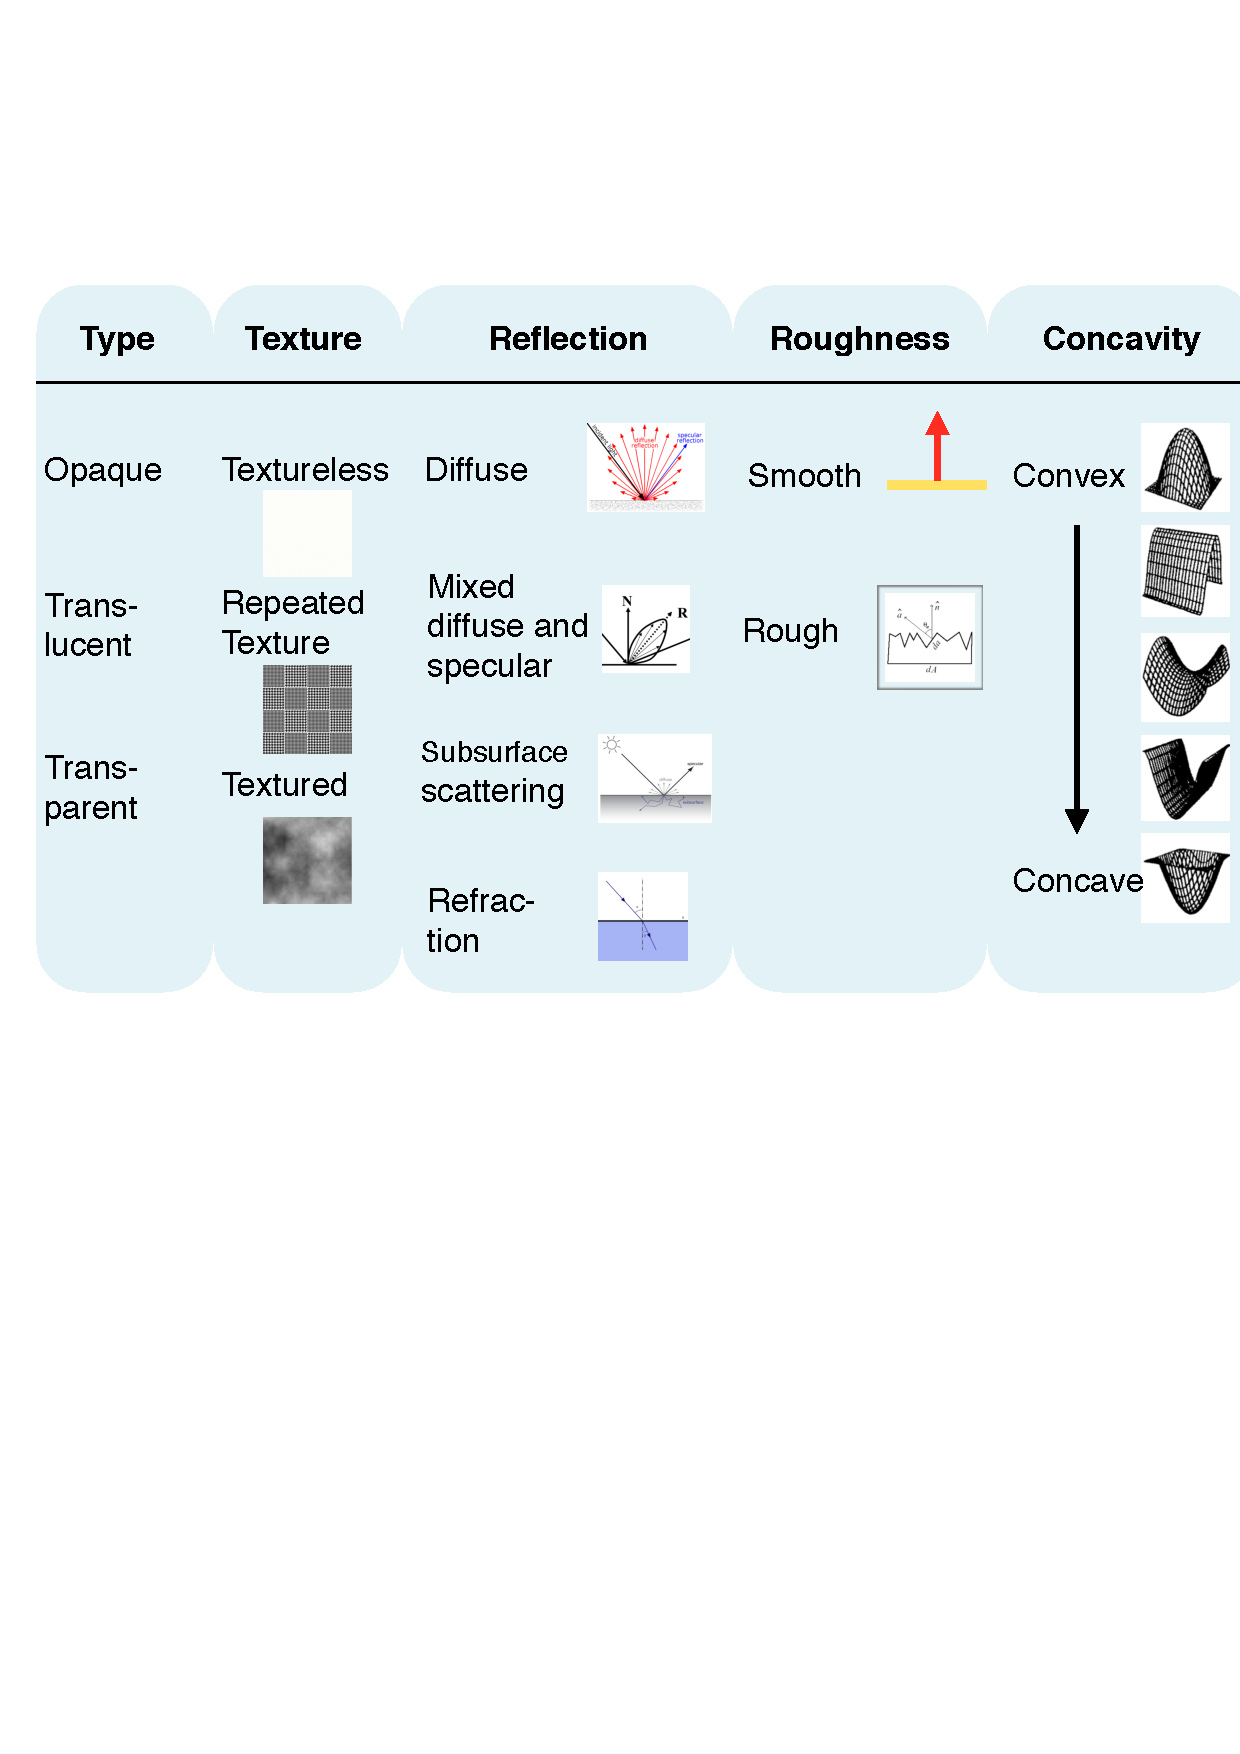
\includegraphics[width=\textwidth]{taxo/obj_class}\\
\caption{A list of properties for object classes.}
\label{fig:obj_class}
\end{figure}

\subsubsection{Class labels}
\begin{itemize}
\item \textbf{Translucency}: \textbf{O}: opaque, \textbf{Tl}: translucent, \textbf{Tp}: transparent.
\item \textbf{Texture}: \textbf{T}: textured, \textbf{Tr}: repeated textured, \textbf{Tl}: textureless.
\item \textbf{Lightness}: \textbf{B}: bright, \textbf{D}: dark.
\item \textbf{Reflection}: \textbf{D}: diffuse model, \textbf{S}: specular model, \textbf{M}: mixture of diffuse and specular, \textbf{Ss}: subsurface scattering, \textbf{Rf}: refraction
\item \textbf{Roughness}: \textbf{S}: smooth, \textbf{R}: rough
\item \textbf{Concavity}: \textbf{Cx}: convex, \textbf{Cv}: concave
\end{itemize}

\begin{table}[!htbp]
\centering
\begin{tabular}{l|*{6}{c}}
\toprule
Class \# & Translucency & Texture & Lightness & Refection & Roughness & Concavity\\
\midrule
1 & O & Tl & B & D & R & Cx\\
2 & O & Tl & B & M & S & Cx\\
3 & O & T & B & D & R & Cx\\
4 & O & T & B & M & S & Cx\\
5 & O & T & D & D & S & Cx\\
6 & O & T & D & M & S & Cx\\
\bottomrule
\end{tabular}
\caption{Label of six classes of objects.}
\label{tab:six_obj_class}
\end{table}

\subsubsection{A traditional taxonomy}
Traditionally, algorithms are categorized into different classes based on the visual cues used for reconstruction, as discussed in Chapter~\ref{ch:RelatedWork}. 
Table~\ref{tab:class_algo} gives an example of what a typical taxonomy would look like.
\begin{table}[!htbp]
  \centering
  \begin{tabular}{l|l}
  \toprule
  \textbf{Algo. class} & \textbf{Technique}\\
  \midrule
  SfS & Horn~\cite{horn1970shape}\\
  MVS & Furukawa~\cite{furukawa2010accurate}, Goesele~\cite{goesele2006multi}, Vogiatzis~\cite{vogiatzis2007multiview}, \\
      & Hern{\'a}ndez~\cite{esteban2004silhouette}, Faugeras~\cite{faugeras2002variational}\\
  Lamberian PS & Woodham~\cite{woodham1980photometric}, Hayakawa~\cite{hayakawa1994photometric}, Belhumeur~\cite{belhumeur1999bas}, \\
      & Alldrin~\cite{alldrin2007resolving}\\
  Non Lambertian PS & Coleman~\cite{coleman1982obtaining}, Barsky~\cite{barsky20034}, Schluns~\cite{schluns1993photometric}, Sato~\cite{sato1994temporal}, \\
      & Mallick~\cite{mallick2005beyond}, Alldrain~\cite{alldrin2008photometric}, Goldman~\cite{goldman2010shape}, Silver~\cite{silver1980determining}, \\
      & Hertzmann~\cite{hertzmann2005example}, Zickler~\cite{zickler2002helmholtz}\\
  % MVPS & \checkmark & \\
  SL & Inokuchi~\cite{inokuchi1984range}\\
  VH & Szeliski~\cite{szeliski1993rapid}, Matusik~\cite{matusik2002efficient}, Tarini~\cite{tarini2002marching}\\
  \bottomrule
  \end{tabular}
  \caption{A traditional taxonomy that classifies algorithms based on algorithmic details.}
  \label{tab:class_algo}
\end{table}

\section{Working conditions of algorithms}
This section investigates the cases where each category of algorithms is capable of working under based on the reported literature. Only visual texture is considered, and it can be thought of as a pattern or variance of intensity appearing on an object's surface. In this thesis, the visual texture will be considered as resulting from non-uniform surface albedo. Thus, uniform albedo represents uniform texuture while non-uniform albedo represents textured surfaces.

\subsection{Multi-view Stereo}
The working conditios of Multi-view Stereo algorithms are summarized in Table~\ref{tab:mvs_cond}. For a typical MVS algorithm to perform well, the object should have a textured and diffuse surface.

\subsubsection{High texture}
Multi-view Stereo algorithms take advantage of textural information to establish point correspondences across different views. Thus homogeneous surfaces pose great challenges to MVS algorithms. However, some MVS algorithms tested on a textureless object ``Dino'' in the Middlebury MVS benchmark~\cite{seitz2006comparison} give successful reconstruction results. This demonstrates that MVS algorithms are able to exploit very weak and intricate image textures, most of which come from shading and/or shadowing effects. However, these texture are so weak that images need to have very high quality.

% \citeauthor{furukawa2008high} use wide-baseline stereo matching to recover the 3D coordinates of salient feature points, then shrink a visual hull model so that the recovered points lie on its surface, then refine the result using energy minimization. \citeauthor{goesele2006multi} compute a depth map from each camera viewpoint (similar to [31]) and merge the results using VRIP [62]. \citeauthor{esteban2004silhouette} first compute a depth map from each camera viewpoint and merge the results into a cost volume. They then iteratively deform a mesh, initialized at the visual hull, to find a minimum cost surface in this volume, also incorporating terms to fit silhouettes. Kolmogorov and Zabih [35] compute a set of depth maps using multi-baseline stereo with graph cuts, then merge the results into a voxel volume by computing the intersections of the occluded volumes from each viewpoint. \citeauthor{faugeras2002variational} compute a minimum cost surface by evolving a surface in a level-set frame-work, using a prediction-error measure. \citeauthor{vogiatzis2007multiview} compute a correlation cost volume in the neighborhood of the visual hull. A minimum-cost surface is then computed using volumetric min-cut.

\subsubsection{Diffuse reflectance}
Most MVS algorithms require that the object surface with similar or same appearances from different perspectives, and hence, most of the algorithms assume Lambertian reflectance. While pure Lambertian surfaces are rare in reality, it is empirically verified that MVS algorithms perform reasonably well on non-Lambertian surfaces. As long as the cameras can capture the diffuse reflectance component, and then the photo-consistency function is able to identify and ignore images whose non-diffsue effects (e.g., specular highlights) are strong, then utilize the diffuse component in the remaining images. Further, there are some attempts to overcome this limitation, a pure passive methods was proposed that directly model and analyze non-Lambertian effects for MVS algorithms~\cite{jin2003multi,jin2005multi}.
\begin{table}[!htbp]
  \centering
  \begin{tabular}{l*{5}{p{15mm}}}
  \toprule
  \textbf{Technique} & Texture & Lightness & Reflectance & Roughness & Concavity\\
  \midrule
  MVS & Textured & - & Diffuse or mixed & - & -\\
  \bottomrule
  \end{tabular}
  \caption{Working condition of Multi-view Stereo algorithms.}
  \label{tab:mvs_cond}
\end{table}

\subsection{Shape from Shading}
Shape from Shading, first proposed by Horn~\cite{horn1970shape}, specifically targets isotropic, known Lambertian surfaces. By assuming orthographic projection, and known light source intensity and direction, surface orientation can be estimated from shading variations. The working condition is shown in Table~\ref{tab:sfs_cond}.

\subsubsection{Reflectance model}
Though other reflectance models are feasible, typical SfS algorithms assume Lambertian reflectance model. The reason is that surface lightness is directly related to surface orietation and reflectance model once the light source and viewing direction are fixed. This is generally an ill-posed problem even with the simplest reflectance model since there is only one intensity value per pixel to solve for surface orientation, which has two DoF. However, even in the simplest case, the survey by Zhang~\cite{zhang1999shape} demonstrate that SfS algorithms generally perform poorly, and none performs well in all cases.

\subsubsection{Interreflection}
Typical SfS algorithms cannot deal with interreflections, since the surface lightness would be corrupted by light transport between surface facets. Thus, object exhibit any form of concavity will pose great challenge to SfS algorithms.

\begin{table}[!htbp]
  \centering
  \begin{tabular}{l*{5}{p{15mm}}}
  \toprule
  \textbf{Technique} & Texture & Lightness & Reflectance & Roughness & Concavity\\
  \midrule
  SfS & Textureless & Bright & Lambertian & Smooth & Convex\\
  \bottomrule
  \end{tabular}
  \caption{Working condition of Shape from Shading algorithms.}
  \label{tab:sfs_cond}
\end{table}

\subsection{Photometric Stereo}
Photometric Stereo can be considered as an extension of SfS algorithms, which adds additional light sources to remove the ambiguity faced by SfS algorithms. The working conditions of Photometric Stereo algorithms are summarized in Table~\ref{tab:ps_cond}.

\subsubsection{Albedo}
Photometric Stereo algorithms work more reliably on surfaces with sufficiently strong albedo. This is because the algorithm exploits the intensity variation as a visual cue, which is more challenging to detect on surfaces with low intensity values.

Though SfS algorithms requires uniform albedo, typical PS algorithms can be used easily on surfaces with spatially varying albedo. First the albedo-scaled normal can be estimated, then the albedo is retrieved as the magnitude of the scaled normal~\cite{woodham1980photometric}.

\subsubsection{Lambertian reflectance model} % Lambertian PS: uniform reflectance
The Lambertian PS algorithms can be divided into two group: calibrated method, and uncalibrated method. The original PS proposed by Woodham~\cite{woodham1980photometric} can be considered as calibrated Lambertian PS. Later, more uncalibrated Lambertian PS have been proposed to avoid this tedious process.

Silver~\cite{silver1980determining} proposed a look-up scheme that relies on a reflectance object with the same reflectance as the target, which in this case is a uniform Lambertian surface. This approach is later adapted to surface with non-Lambertian reflectance with varying albedo or material in~\cite{hertzmann2005example}.

Another successful uncalibrated approach used six or more pixels with the same albedo, and was able to solve for normals up to a rotation ambiguity\cite{hayakawa1994photometric}. It can be further proved that a 3-parameter subset of these transformations, known as the Generalized Bas-Relief (GBR) ambiguity, preserve surface integrability~\cite{belhumeur1999bas}. Thus, given three or more imges of a Lambertian object acquired under light sources of unknown direction and strength, the surface can be reconstructed up to GBR transformation by enforcing surface integrability, see Figure~\ref{fig:gbr} for the effect of GBR-ambiguity.
\begin{figure}[!htbp]
\centering
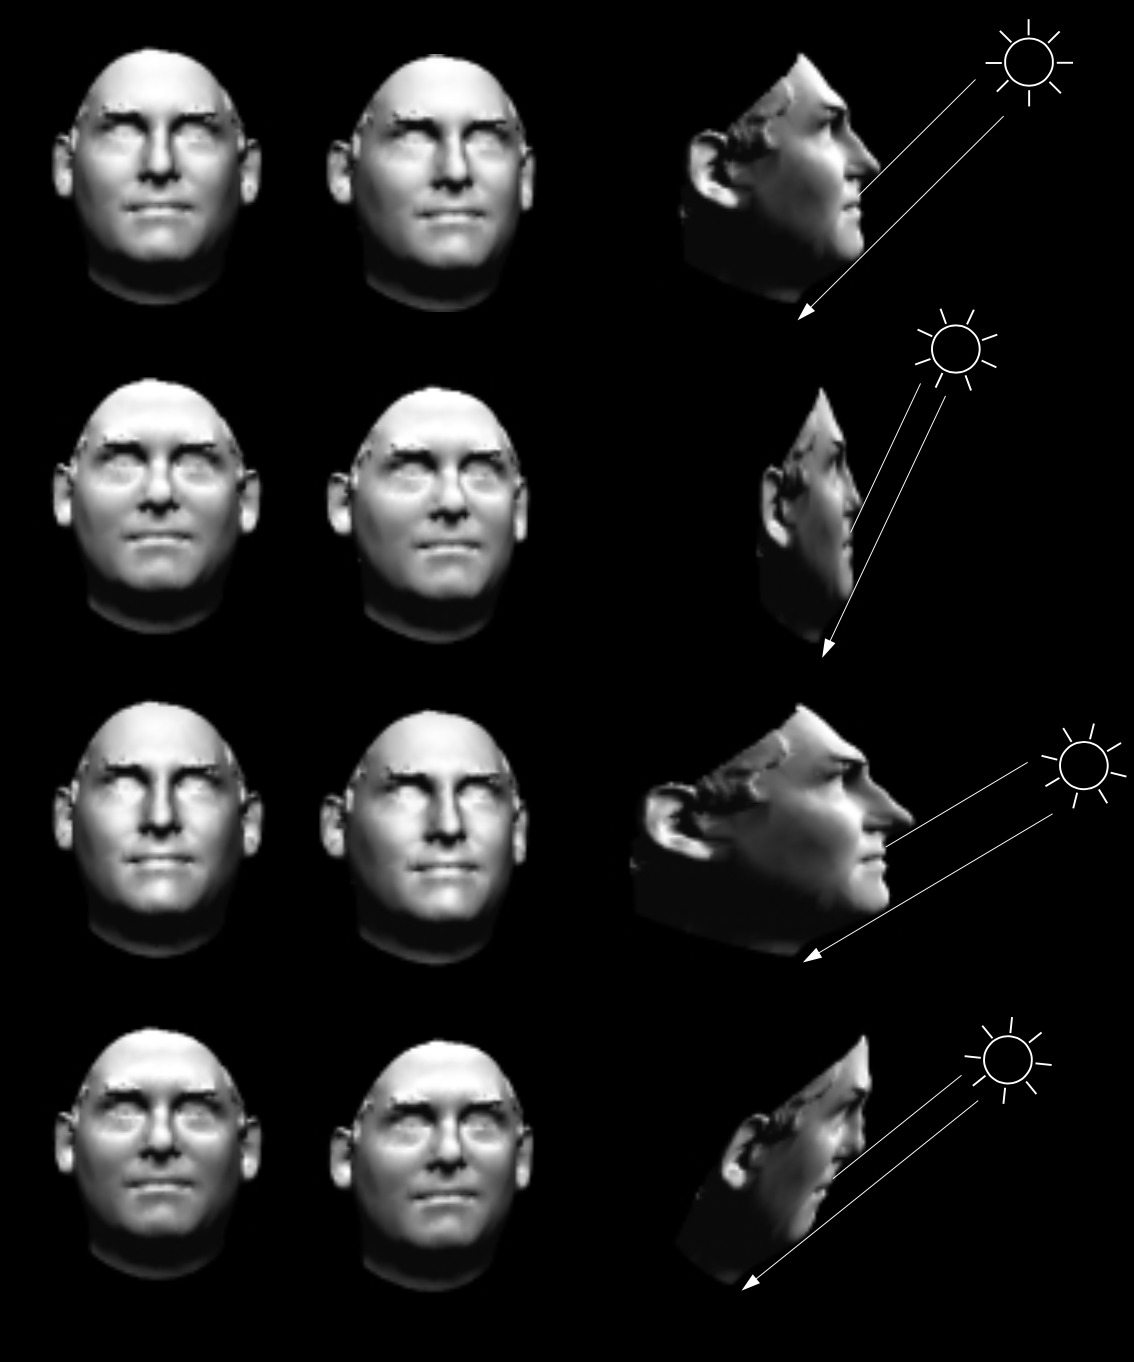
\includegraphics[width=0.6\textwidth]{taxo/gbr.png}
\caption{The effect of GBR ambiguity. Two sets of shape and light source configurations can produce exactly the same images.}
\label{fig:gbr}
\end{figure}

\subsubsection{Non-Lambertian reflectance model}
Much of the emphasis in PS has been to relax the assumption of Lambertian reflectance. There are four classes of Non-Lambertian PS algorithms: the first class treats specular component as outliers~\cite{coleman1982obtaining,barsky20034,ikeuchi1981determining,nayar1990determining}; the second class uses reference object that has the same material as the target object~\cite{hertzmann2005example}; the third class assumes that the reflectance can be modeled as a linear combination of a set of basis reflectance models~\cite{goldman2010shape,alldrin2008photometric}; and the fourth class exploits the physical properties common to large classes of BRDFs, such as energy-conservation, non-negativity, Helmholtz reciprocity, isotropy, and so on~\cite{zickler2002helmholtz,tan2007isotropy,alldrin2007toward}.

% One line of approaches exploit the observation that the reflectance of many material can be approximated by the sum of a specular and a diffuse lobe.
% The \textit{reference object} approach, first proposed by~\citeauthor{silver1980determining}, and later revisited by in~\cite{hertzmann2005example}, can be used for surfaces with spatially varying reflectance. The basic assumption is that the BRDF at each point is a linear combination of the ``basis'' BRDFs defined by the set of reference objects.

% One approach exploits the fact that the reflectance of non-Lambertian surfaces can be approximated by \textbf{diffuse component and specular lobe}. \citeauthor{coleman1982obtaining} and \citeauthor{barsky20034} who treat specular pixels as outliers, and \citeauthor{schluns1993photometric}, \citeauthor{sato1994temporal}, and \citeauthor{mallick2005beyond} who assume the color of the specular lobe differs from the color of the diffuse lobe, allowing separation of the specular and diffuse components.

% Due to the high complexity of the BRDF, some methods utilize {analytical reflectance models}. \citeauthor{goldman2010shape} uses an isotropic Ward model for each basis BRDF, and the surface orientation and parameters of the reflectance models are estimated iteratively. \citeauthor{alldrin2008photometric} proposed a data-driven approach that got rid of the parametric reflectance model, and employed an novel bi-variate approaximations of isotropic reflectance functions. By combining this approximation with the weighted basis BRDFs, a per-pixel surface normal, global set of non-parametric basis BRDFs, and the corresponding weights are able to be independently estimated. Though the parametric reflectance model can significantly reduce the complexity of BRDFs, they are typically restricted to a limited classes of materials.

% Another alternative to using BRDF models is to take advantage of the properties of BRDFs, include energy conservation, non-negativity, Helmholtz reciprocity, or isotropy. Helmholtz stereopsis introduced by~\citeauthor{zickler2002helmholtz} exploits the reciprocity to obtain the surface reconstruction. Isotropy is another physical property which holds for material without ``grain''. \citeauthor{tan2007isotropy} use both symmetry and reciprocity present in isotropic BRDFs to resolve the generalized bas-relief ambiguity. \citeauthor{alldrin2007toward} show that isotropy, with no further assumptions on surface shape or BRDF, can be utilized to recover the surface normal at each surface point up to a plane.

% A four-source photometric stereo technique uses a fourth source of illumination to detecta and remove specular reflections~\cite{coleman1982obtaining}. By adding a fourth image, it's possible to compute four sets of normals, \ie one normal for each permutation of three intensity values. If there is a greater deviation in both magnitude and direction of the normals, a method can now be developed to eliminate specular effects using a thresholding procedure.

\subsubsection{Convexity}
Active methods that assumes a local reflectance model such as most PS algorithms can work more reliably on surfaces without casting shadow and interreflection. Thus surfaces with concavities pose a great challenge for this type of techniques since the indensity can be affected by other surface patches.

\begin{table}[!htbp]
  \centering
  \begin{tabular}{p{3cm}*{5}{p{15mm}}}
  \toprule
  \textbf{Technique} & Texture & Lightness & Reflectance & Roughness & Concavity\\
  \midrule
  Lambertian PS, uniform albedo & Textureless & Bright & Lambertian & - & Convex\\
  Lambertian PS, non-uniform albedo & Textured & Bright & Lambertian & - & Convex\\
  Non-Lambertian PS & - & Bright & Mixed & - & Convex\\
  \bottomrule
  \end{tabular}
  \caption{Working conditions of typical Photometric Stereo algorithms.}
  \label{tab:ps_cond}
\end{table}

\subsection{Structured Light}
For stereo correspondence based methods, actively projected patterns have to be used for the lack of surface texture. Since the surface is diffuse, there is no specular reflection to cause severe noise. Refer to Table~\ref{tab:sl_cond} for the working condition of SL.

\subsubsection{High albedo}
Regardless of what projection pattern is used, the most important feature of most SL techniques is that it should be able to determine if a surface point is lit or not. Thus, the surface albedo needs to be strong enough so that sufficient amount of reflected light can reach the camera sensor.

\subsubsection{Diffuse reflectance model}
Traditional Structured Light techniques cannot deal with highly specular surfaces since the specular area will exhibit strong reflection even for low lighting conditions, which will cause errors in the encoding process.

\subsubsection{Concexity}
Active methods that assumes a local reflectance model such as SL algorithms can work more reliably on surfaces without casting shadow and interreflection. Thus surfaces with concavities pose a great challenge for this type of techniques since the indensity can be affected by other surface patches.
\begin{table}[!htbp]
  \centering
  \begin{tabular}{c*{5}{p{15mm}}}
  \toprule
  \textbf{Technique} & Texture & Lightness & Reflectance & Roughness & Concavity\\
  \midrule
  Structured Light & - & Bright & Lambertian & - & Convex\\
  \bottomrule
  \end{tabular}
  \caption{Working condition of typical Structured Light algorithms.}
  \label{tab:sl_cond}
\end{table}

\subsection{Visual Hull}
Visual Hull algorithms don't rely on material properties as long as the foreground of the image can be reliably segmented, thus is applicable for objects with arbitrary visual properties. However, it fails to carve the concavities on the object surface, thus is unsuitable to concave objects.
\begin{table}[!htbp]
  \centering
  \begin{tabular}{c*{5}{p{15mm}}}
  \toprule
  \textbf{Technique} & Texture & Lightness & Reflectance & Roughness & Concavity\\
  \midrule
  VH & - & - & - & - & Convex\\
  \bottomrule
  \end{tabular}
  \caption{Working condition of typical Visual Hull algorithms.}
  \label{tab:ps_cond}
\end{table}
% \begin{table}[!htbp]
%   \centering
%   \begin{tabular}{l*{2}{c}}
%   \hline
%   \textbf{Technique} & Representation & Algorithm\\
%   \hline
%   Szeliski~\cite{szeliski1993rapid} & 3D grids & Voxel-based\\
%   Tarini~\cite{tarini2002marching} & 3D rays & MI-based\\
%   Matusik~\cite{matusik2002efficient} & Polygonal mesh & Exact polyhedral methods\\
%   \hline
%   \end{tabular}
%   \caption{Summary of VH representations and reconstruction approach.}
%   \label{tab:summary_class_6}
% \end{table}

\section{Summary}
Our taxonomy categorizes algorithms based on the problem conditions that they can reliably work under. The problem conditions consists of various visual and geometric properties, as shown in Figure~\ref{fig:obj_class}. These properties can be conceptualized as dimensions of the 3D reconstruction problem space. This taxonomy provides an abstraction which allows us to think of algorithms as volumes within a $n-$dimensional problem space. Existing algorithms can be introduced into this framework based on the performance within the problem space. The aforementioned analysis provide an initial mapping of the space that is summarized below in Figure~\ref{fig:six_class}, and more in detail in Table~\ref{tab:algo_taxo}.
\begin{figure*}[!htbp]
\centering
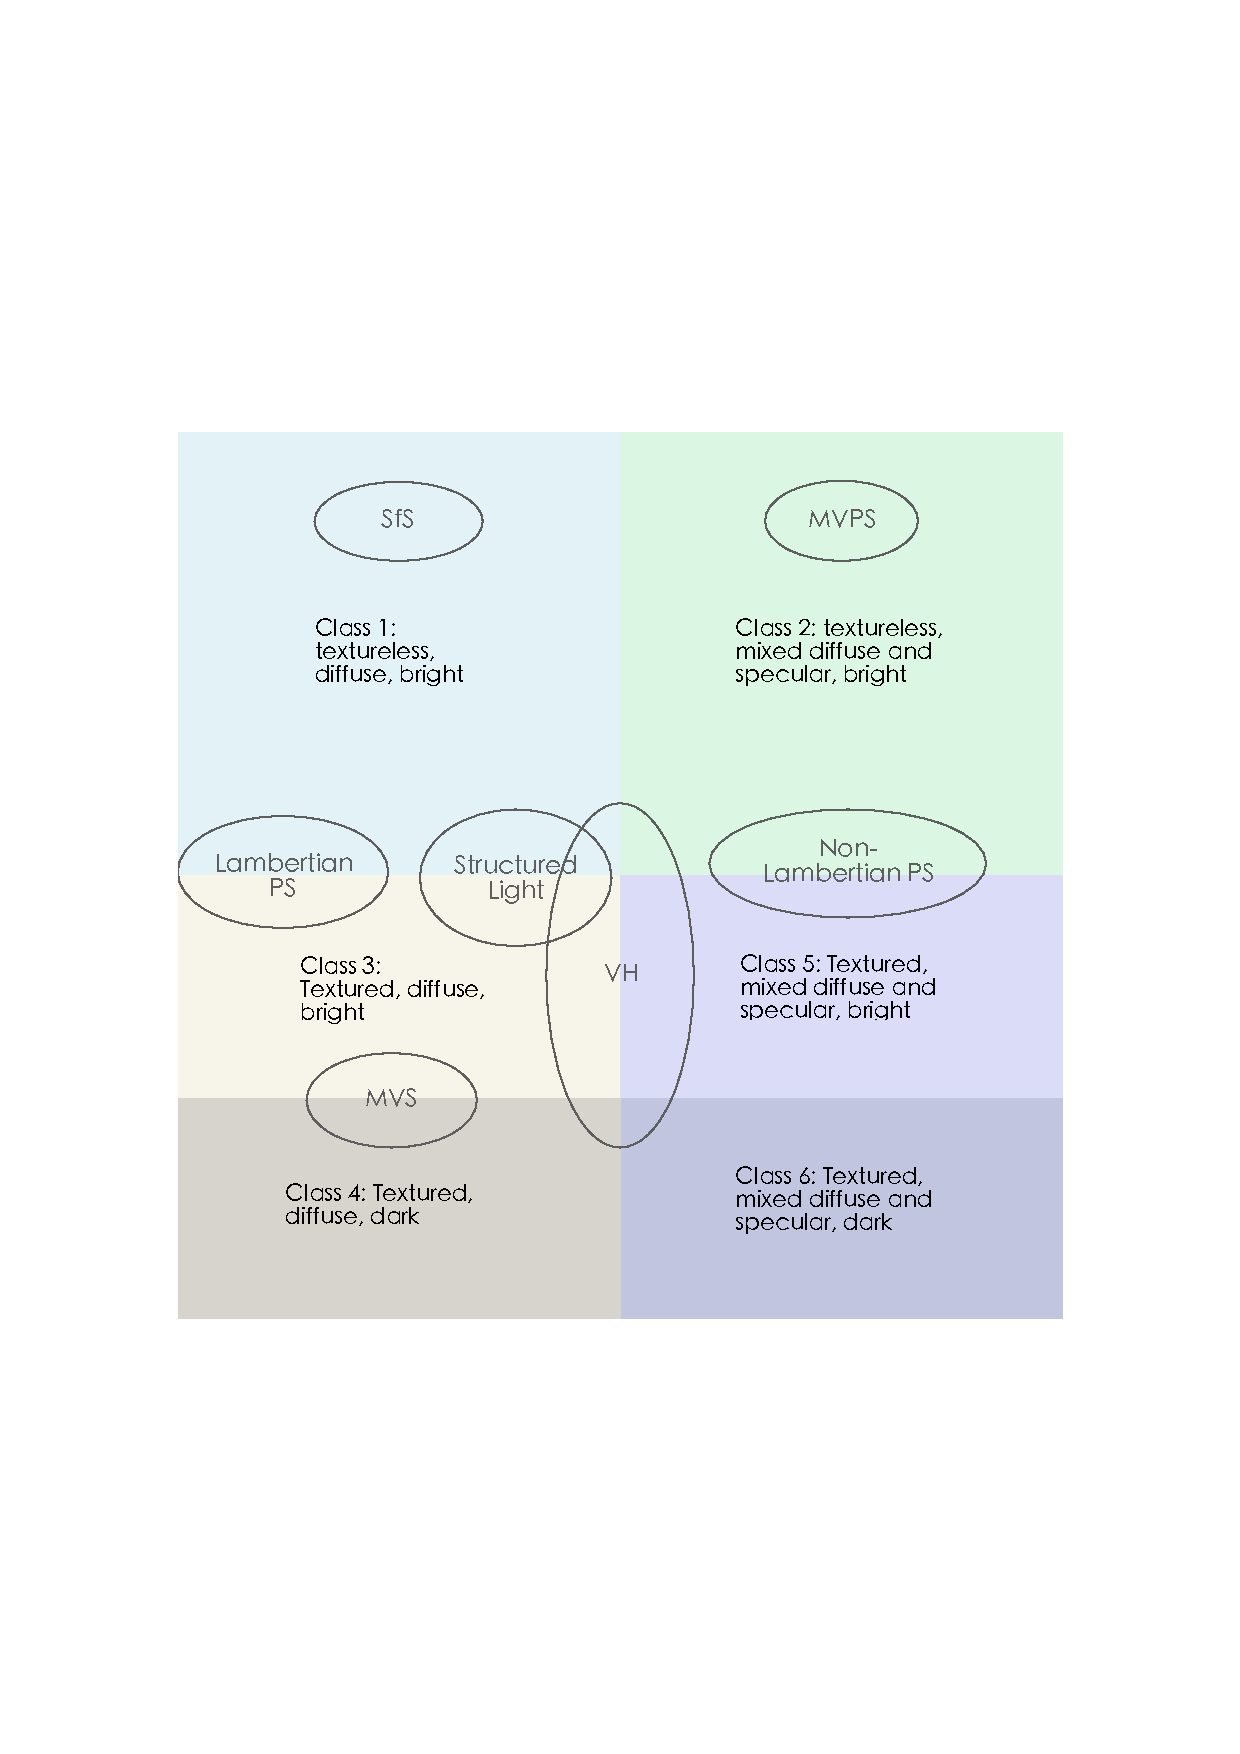
\includegraphics[width=0.5\textwidth]{taxo/six_class}
\caption{Six classes of objects of interest, and the algorithms that could work reliably for these classes.}
\label{fig:six_class}
\end{figure*}

\begin{table}[!htbp]
  \centering
  \begin{tabular}{l|l|p{10cm}}
  \toprule
  \textbf{Class \#} & Class label & Algorithms\\
  \midrule
  1 & \textbf{OTlBDRCx} & Horn~\cite{horn1970shape}, Woodham~\cite{woodham1980photometric}, Hayakawa~\cite{hayakawa1994photometric}, Belhumeur~\cite{belhumeur1999bas}, Alldrin~\cite{alldrin2007resolving}\\
  2 & \textbf{OTlBMSCx} & Coleman~\cite{coleman1982obtaining}, Barsky~\cite{barsky20034}, Schluns~\cite{schluns1993photometric}, Sato~\cite{sato1994temporal}, Mallick~\cite{mallick2005beyond}, Alldrain~\cite{alldrin2008photometric}, Goldman~\cite{goldman2010shape}, Silver~\cite{silver1980determining}, Hertzmann~\cite{hertzmann2005example}, Zickler~\cite{zickler2002helmholtz}\\
  3 & \textbf{OTBDRCx} & Woodham~\cite{woodham1980photometric}, Hayakawa~\cite{hayakawa1994photometric}, Belhumeur~\cite{belhumeur1999bas}, Alldrin~\cite{alldrin2007resolving}, Furukawa~\cite{furukawa2010accurate}, Goesele~\cite{goesele2006multi}, Vogiatzis~\cite{vogiatzis2007multiview}, Hern{\'a}ndez~\cite{esteban2004silhouette}, Faugeras~\cite{faugeras2002variational}, Inokuchi~\cite{inokuchi1984range}\\
  4 & \textbf{OTBMSCx} & Furukawa~\cite{furukawa2010accurate}, Goesele~\cite{goesele2006multi}, Vogiatzis~\cite{vogiatzis2007multiview}, Hern{\'a}ndez~\cite{esteban2004silhouette}, Faugeras~\cite{faugeras2002variational}\\
  5 & \textbf{OTDDSCx} & Coleman~\cite{coleman1982obtaining}, Barsky~\cite{barsky20034}, Schluns~\cite{schluns1993photometric}, Sato~\cite{sato1994temporal}, Mallick~\cite{mallick2005beyond}, Alldrain~\cite{alldrin2008photometric}, Goldman~\cite{goldman2010shape}, Silver~\cite{silver1980determining}, Hertzmann~\cite{hertzmann2005example}, Zickler~\cite{zickler2002helmholtz}\\
  6 & \textbf{OTDMSCx} & Szeliski~\cite{szeliski1993rapid}, Matusik~\cite{matusik2002efficient}, Tarini~\cite{tarini2002marching}\\
  \bottomrule
  \end{tabular}
  \caption{Algorithm classification based on the proposed taxonomy.}
  \label{tab:algo_taxo}
\end{table}
%% The following is a directive for TeXShop to indicate the main file
%%!TEX root = diss.tex

\chapter{Model of 3D Reconstruction}
\label{ch:3DRecon_Model}
In Chapter~\ref{ch:3DRecon_Taxo}, we introduce a taxonomy of 3D reconstruction which map algorithms according to the main visual cues used for reconstruction. In this chapter, we attempt to extend this mapping by providing a model of 3D reconstruction which allows for a well defined specification of the visual cues surrounding the problem and of the range of the desired solution, abstracting away from the functional specification of \textit{how} to estimate a reconstruction.

The goal when providing an abstraction to 3D reconstruction is that with better description should lead to better result. To order to achieve this, the visual and geometric properties of an object that can affect the visual cues should be examined in depth so that important aspects of the problem can be described.

A key requirement of the 3D reconstruction model is that it should be interpretable. Thus the components of this model must be well defined. We first propose a formal definition of the 3D reconstruction problem in Section~\ref{sec:3DRecon_Def}. Section~\ref{sec:3DRecon_Rep} explores the inputs and outputs used in 3D reconstruction problems. Section~\ref{sec:3DRecon_Desc} discusses various \textit{properties} that can be used to describe the appearance of the object. Section~\ref{sec:3DRecon_Exp} provides the mapping of the representations and properties into a formal model via which 3D reconstruction problem can be expressed. These layers: Definition, Representation, Conditions, and Expression represent out framework of accessible 3D reconstruction.

\section{Definition}
\label{sec:3DRecon_Def}
We first give the definition of some basic concepts, which encompass general computer vision concepts such as scene, camera, and image. We then define some other notions that are close related to the reconstruction problem before a formal definition is introduced. We then provide some reasonable approximations for a more practical definition.

\subsection{Basic notations}
We use the following notations: $\{C_n\}_{n=0}^{N-1}$ represents the camera set, which include both the intrinsic and extrinsic parameters; $\{I_n\}_{n=0}^{N-1}$ represents the set of all images; $\{L_n\}_{n=0}^{N-1}$ represents the set of light sources.

\textbf{Definition 1 (Scene)} The scene $S$ is the four-dimensional joint spatio-temporal target of interest.

\textbf{Definition 2 (Image)} The transformation of the scene $S$ onto the image plane of camera $C_i$ at time $t_0$, which can be modelled as: $I_i = T(S, C_i, L_0, t_0)$, or the transformation of the scene $S$ onto the image plane of $C_0$  under the light source $L_i$ at time $t_i$, $I_i= T(S, C_0, L_i, t_i)$, where $T$ is the transformation.

The transformation can be a geometric one which determines the 2D coordinates from a 3D position, or a radiometric one which determines the intensity/irradiance information from the information of illumination, viewing direction and surface orientation, or both.

\subsection{Segment and Scelement}
Segment is the lowest level element in the image, can be considered as a generalized pixel.

\textbf{Definition 3 (Segment)} A segment is a distinct region in the image.

For instance, a segment can be a pixel, a window area, an edge, a contour, or a region of arbitrary size and shape.

\textbf{Definition 4 (Cue)} cues are the visual or geometric characteristics of the segments $seg$ that can be used for reconstruction, denoted as $cue(seg)$.

For instance, the cue can be texture within a window area, intensity/colour value of a pixel, or object contour, etc.

\textbf{Definition (Scelement)} A Scelement (scene element) is a distinct volume in the scene which corresponds to at least one segment, can be considered as a generalization of a voxel.

\textbf{Definition (Property)} Properties are the visual and geometric characteristics of the scelement $slmt$, which would influence the cues of a segment, denoted as $prop(slmt)$.

The property of the scelment can be the visual texture, diffuse albedo, surface orientation, roughness, convacity, etc.

The relation between these notions is shown in Figure~\ref{seg_scelement}.
\begin{figure}[h]
\centering
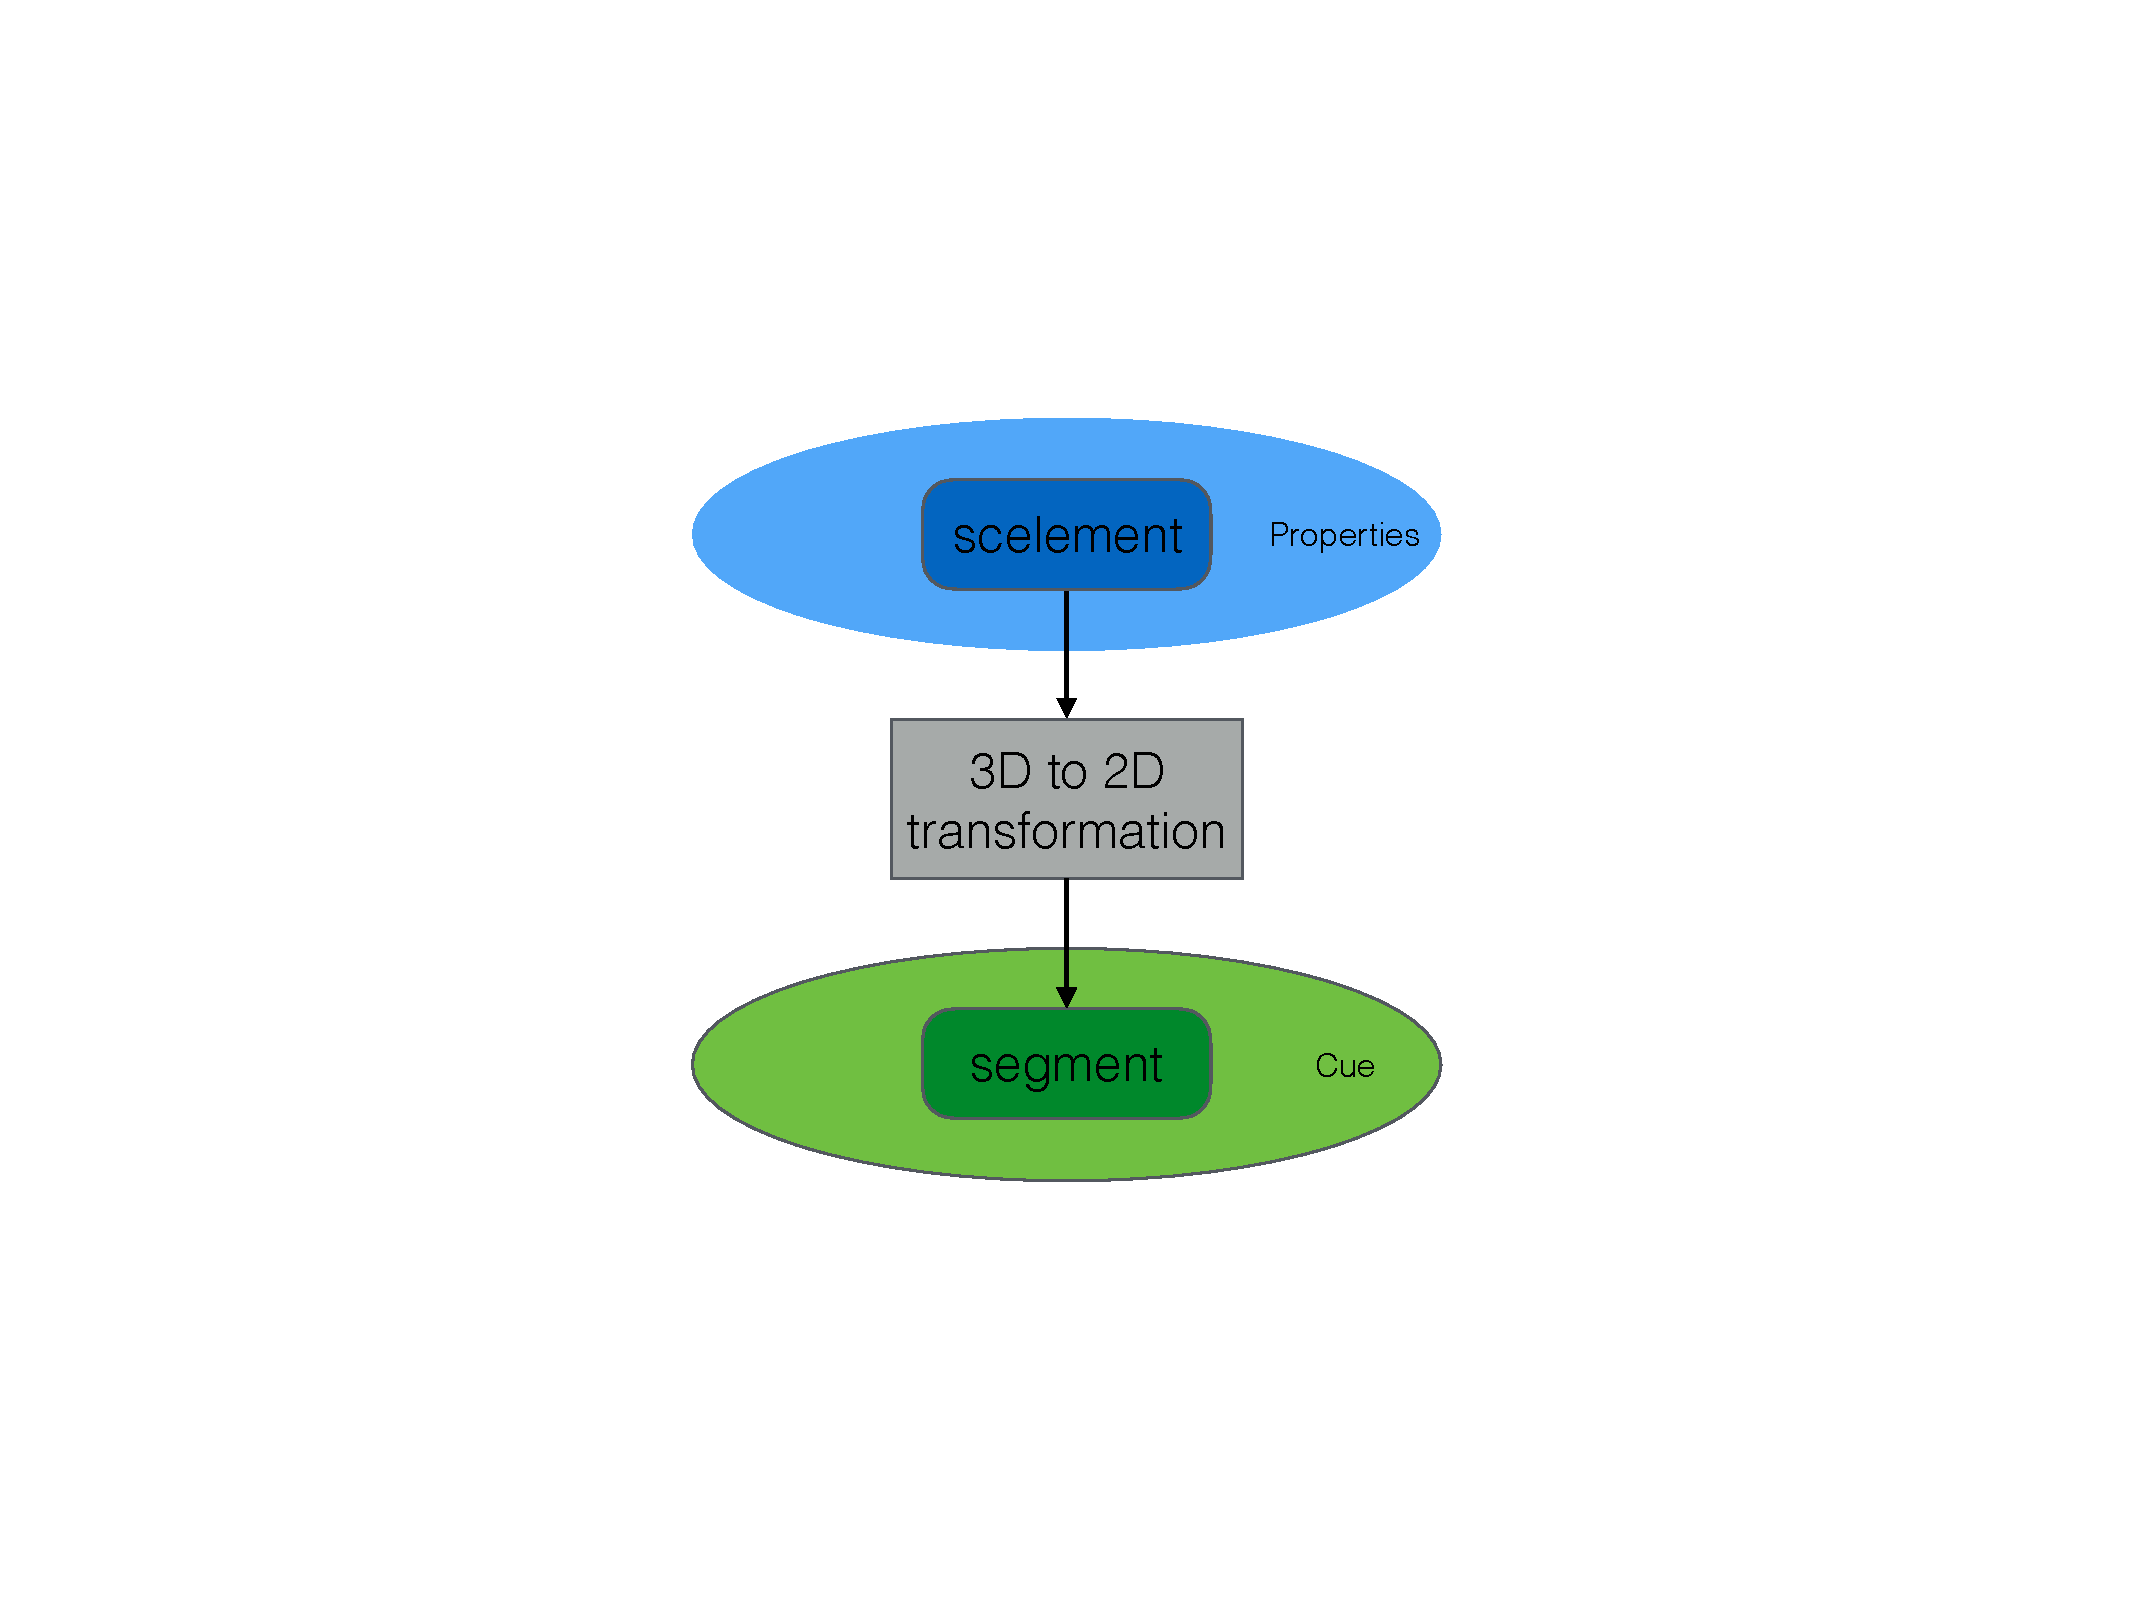
\includegraphics[width=0.5\textwidth]{model/seg_scelement}
\caption{Relation between a scelement and a segment}
\end{figure}

\textbf{Definition (Representation)} The scelement can be represented as a voxel, a depth value, a 3D point/patch, or a surface normal, etc, which is denoted as $rep(slmt)$.

\subsection{Photo-consistency}
Every photograph of a 3D scene taken from a camera $C_i$ partitions the set of all possible shape-radiance scene descriptions into two families, those that reproduce the photograph and those that do not. We characterize this constraint for a given shape and a given radiance assignment by the notion of \textit{photo-consistency}.

\textbf{Definition (Photo-consistency criterion)} The photo-consistency criterion checks whether the properties of a scelement $slmt$ can produce the cues observed in the corresponding segment $seg$.
\begin{align*}
consist(rep(slmt), prop(slmt), cue(seg)) = 1 &\Rightarrow \textit{photo consistent}\\
consist(rep(slmt), prop(slmt), cue(seg)) = 0 &\Rightarrow \textit{not photo consistent}
\end{align*}

\textbf{Definition (Segment photo-consistency)} Let $S$ be the scene. A scelement $s\in S$ that is visible from $C_i$ is photo-consistent with the image $I_i$ if and only if the photo-consistency check is true.

\textbf{Definition (Image photo-consistency)} A scene $S$ is photo-consistent with image $I_i$ if for all scelements $\forall s\in S$ visible from the camera $C_i$ are segment photo-consistent with this image.

\textbf{Definition (Scene photo-consistency)} A scene $S$ is scene photo-consistent with a set of images $\{I_n\}_{n=0}^{N-1}$ if it's image photo-consistency with each image $I_i\in \{I_n\}_{n=0}^{N-1}$ in the set.

\subsection{Formal Definition}
\textbf{Definition (3D reconstruction)} Given a set of images $\{I_n\}_{n=0}^{N-1}$ captured by cameras $\{C_n\}_{n=0}^{N-1}$, or under a set of light sources $\{L_n\}_{n=0}^{N-1}$, find a set of scelements $\{slmt_n\}_{n=0}^{M-1}$ such that any scelement is photo-consistent with the image set $\{I_n\}_{n=0}^{N-1}$, \ie $\forall slmt_i\in \{slmt_n\}_{n=0}^{M-1}$, we have $consist(rep(slmt_i), prop(slmt_i), cue(seg_{(i, n)})) = 1$.

where $seg_{(i, n)}$ is the corresponding segment of $slmt_i$ in camera $C_n$. Alternatively, 3D reconstruction tries to find a set of scelments $\{slmt_n\}_{n=0}^{M-1}$ that are scene photo-consistent with the image set $\{I_n\}_{n=0}^{N-1}$

\subsection{Applied Definition}
While the definition presented above gives an definitive definition of the problem of 3D reconstruction, it does so in a purely theoretical way which is not necessarily applicable in a practical setting. We extend in this section this formal definition to an approximate, but more applied version.

\textbf{Definition (Photo-consistency score)} The photo-consistency score measures the similariy betweem a scelement $slmt$ and the corresponding segment $seg$.
\begin{align*}
consist(rep(slmt), prop(slmt), cue(seg)) &= x \text{, } x\in[0, 1]\\
consist(rep(slmt), prop(slmt), cue(seg)) &= 1 \Rightarrow \textit{photo consistent}\\
consist(rep(slmt), prop(slmt), cue(seg)) &= 0 \Rightarrow \textit{not photo consistent}
\end{align*}

\textbf{Definition (Applied photo-consistency check)} A scelement $slmt$ and a segment $seg$ are considered photo-consistent if the the photo-consistency score is above a pre-defined threshold $\epsilon$.
$$
consist(rep(slmt), prop(slmt), cue(seg)) > \epsilon
$$

\textbf{Definition (Applied 3D Reconstruction)} Given a set of images $\{I_n\}_{n=0}^{N-1}$ captured by cameras $\{C_n\}_{n=0}^{N-1}$, or under a set of light sources $\{L_n\}_{n=0}^{N-1}$, find a set of scelements $\{slmt_n\}_{n=0}^{M-1}$ such that the photo-consistency measure between the set of scelements and their corresponding segments $\{seg_{(i, n)}\}_{i=0,j=0}^{M-1,N-1}$ are maximized.
$$
\mbox{maximize} \quad \sum_{n=0}^{N-1}\sum_{i=0}^{M-1} consist(rep(slmt_i), prop(slmt_i), cue(seg_{(i, n)}))
$$

\section{Representation}
\label{sec:3DRecon_Rep}
Based on the proposed definitions of 3D reconstruction problem, we need to further define the representations so that any developers can express their problem based on our proposed model. We look at the \textit{cues} that are utilized by 3D reconstruction techniques and their corresponding contributing properties. In Chapter~\ref{ch:3DRecon_Taxo}, we explored a new taxonomy of 3D reconstruction based visual/geometric cues. Now we need to investigate the visual and geometric properties of the object that can affect those cues. This section is organized by the visual/geomtric cues, and the visual/geomtric properties are investigated in each section.

\subsection{Segment and scelement}
As defined in section~\ref{sec:3DRecon_Def}, a segment is the 3D to 2D transformation of a scelement. Here we discuss concrete examples of segment and scelement.

\subsubsection{Pixel and voxel}
In the image plane, a pixel is a square of size $1\times 1$. In the matrix representation of an image $I$, a pixel is an entry of the matrix, $I(x, y)$. A voxel is a 3D regular cube, and the center of which is projected to the center of the pixel.
\begin{figure}[h]
\centering
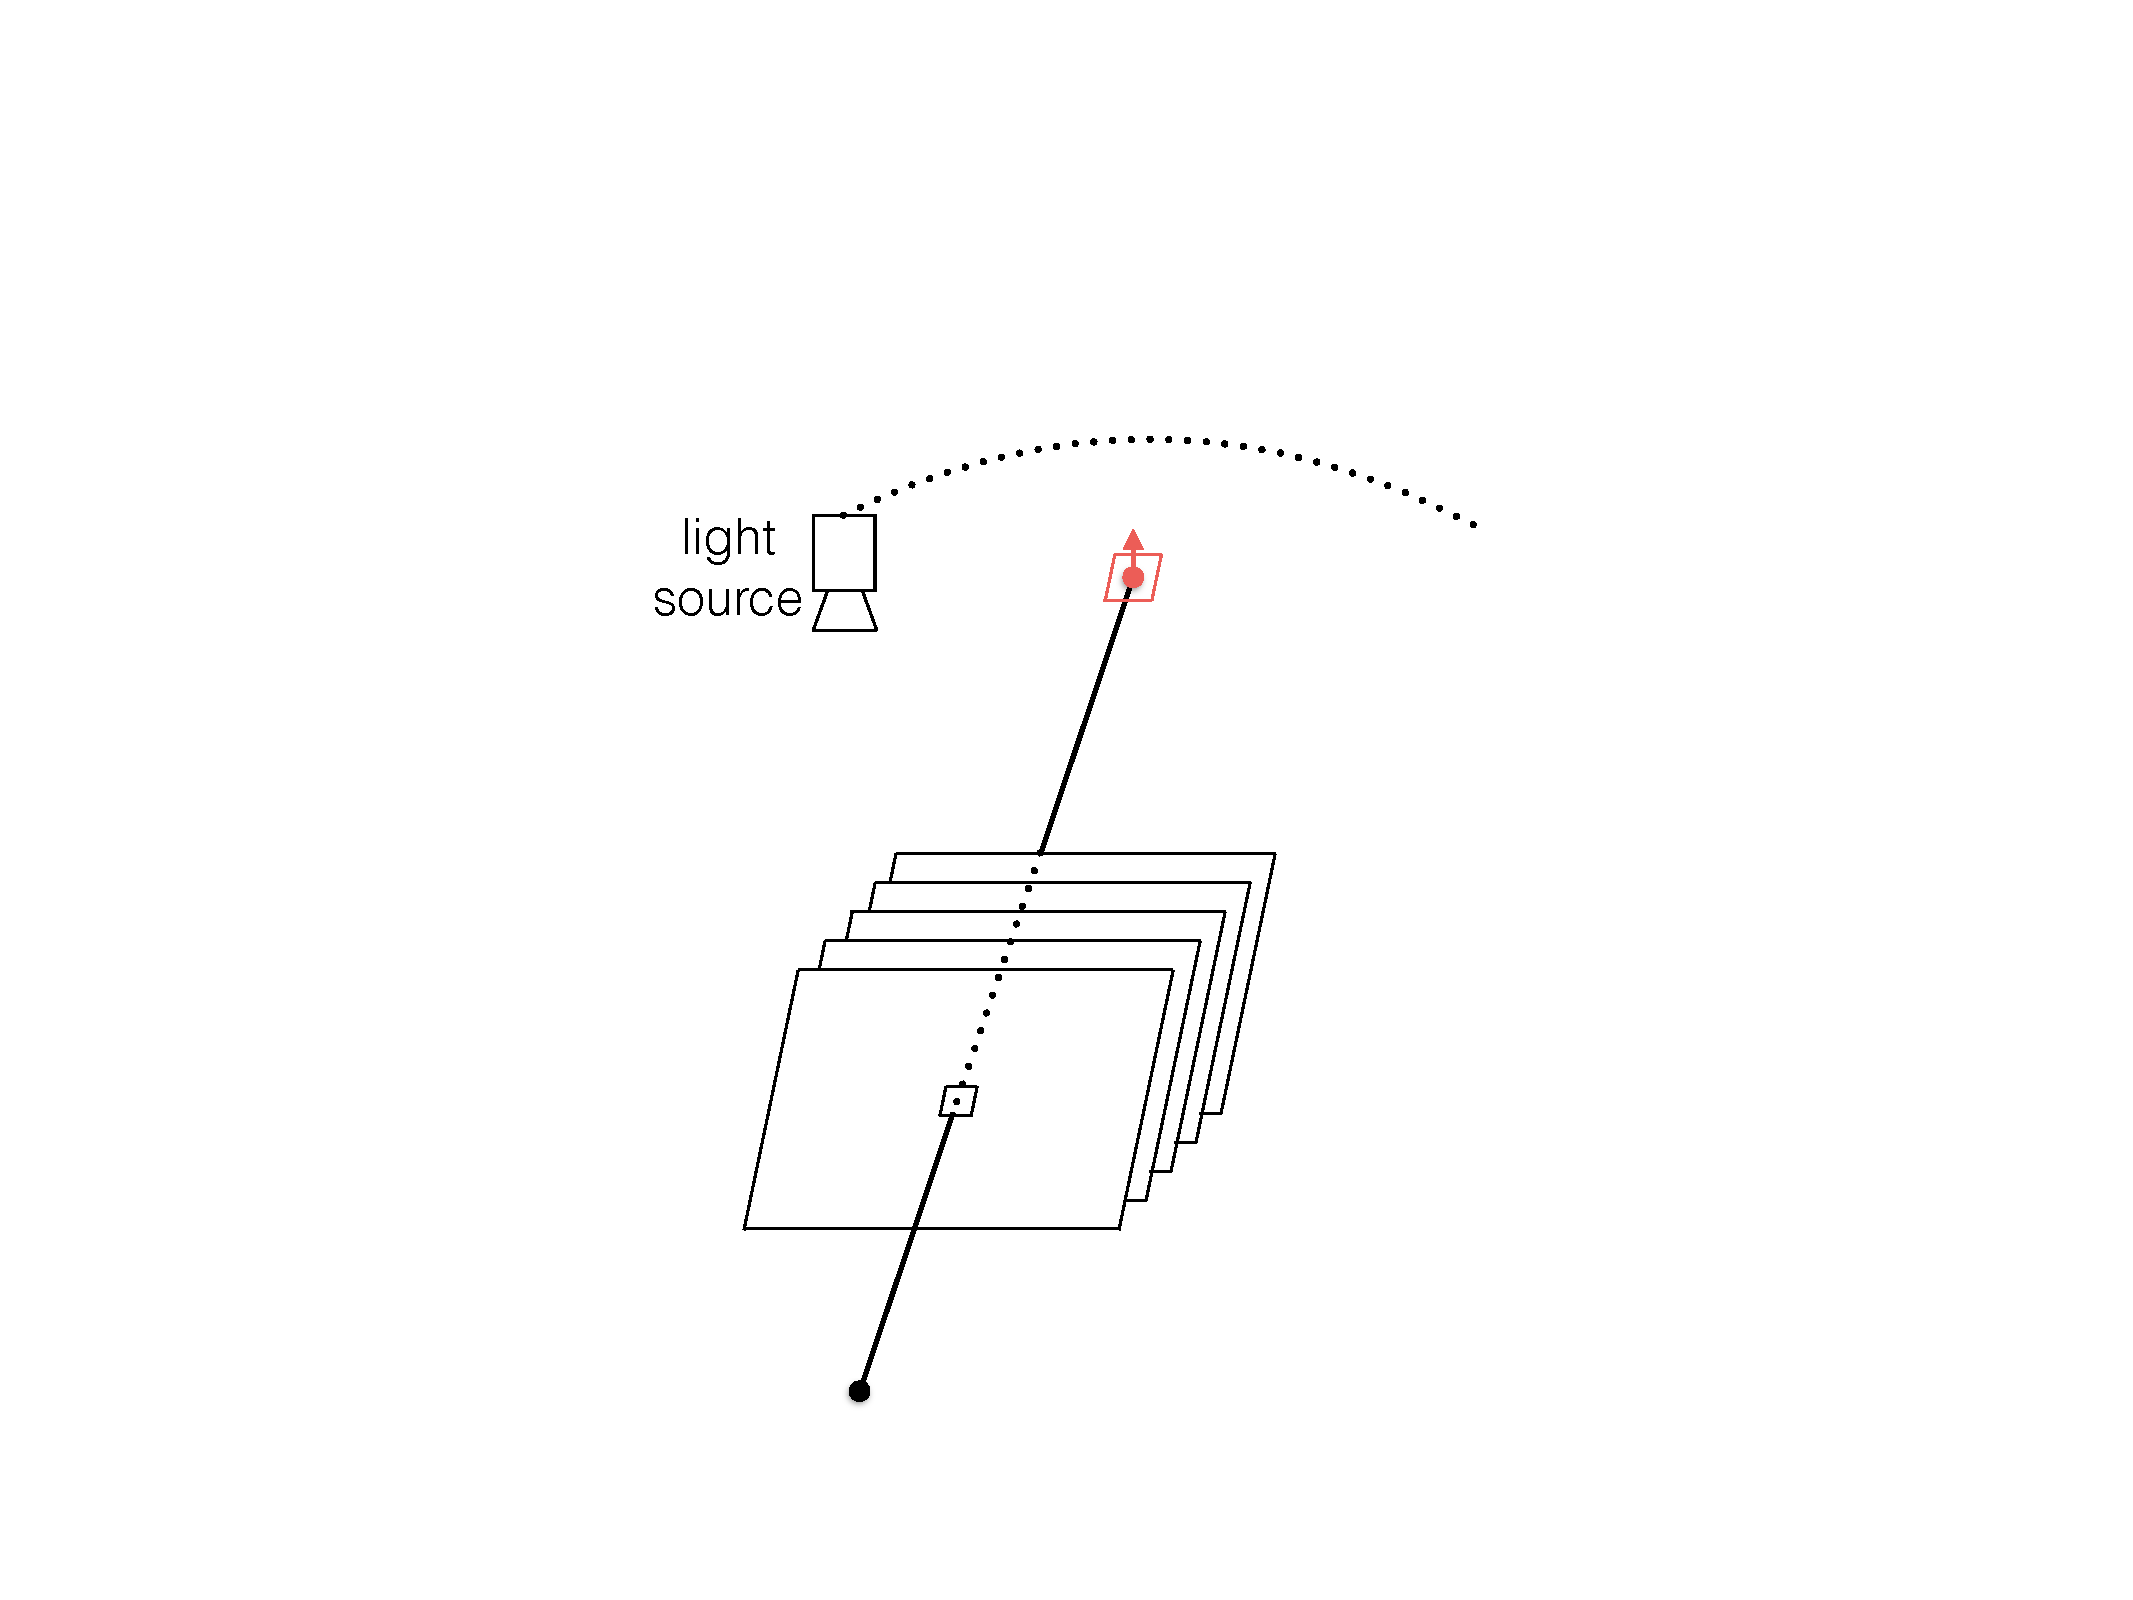
\includegraphics[width=0.6\textwidth]{model/pixel_voxel}
\caption{Pixel and voxel}
\end{figure}

\subsubsection{Silhouette and bounding edge}


\subsubsection{Window area and patch}
A window area is contained in a $w\times w$ regular square, and the surface patch is a 3D point of $p\times p$ with a normal vector.
\begin{figure}[h]
\centering
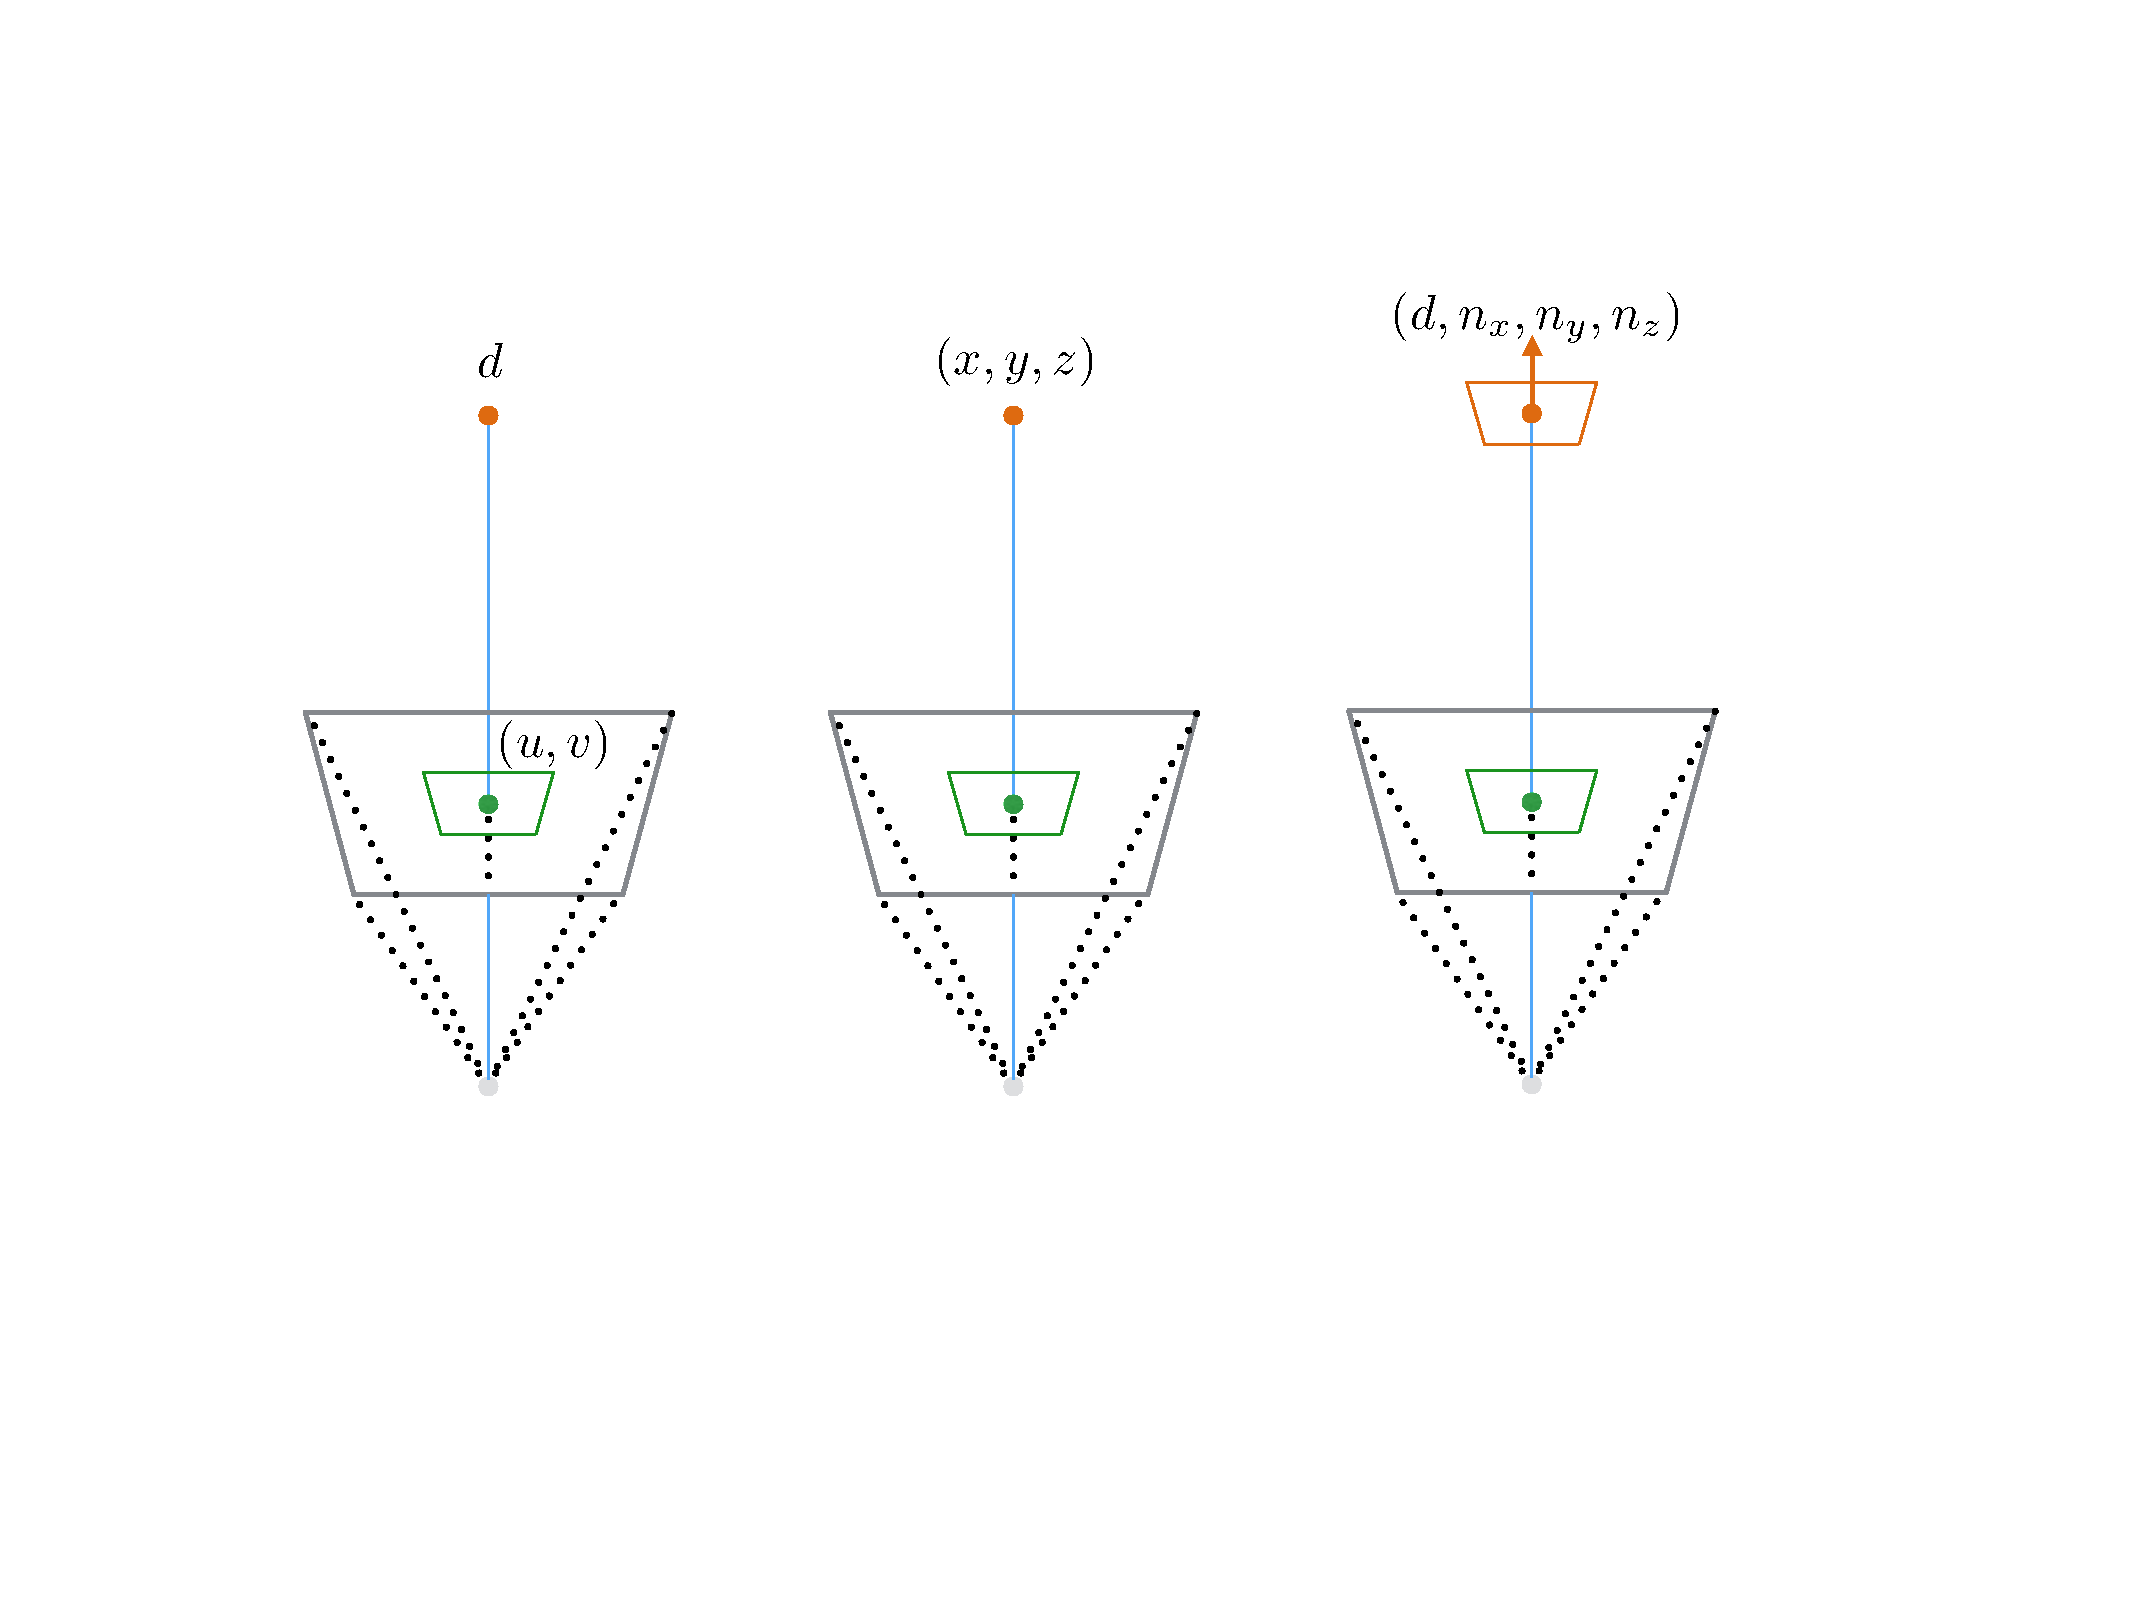
\includegraphics[width=0.8\textwidth]{model/window_patch}
\caption{a window area and a surface patch}
\end{figure}

\subsection{Cues and properties}
As defined in Chapter~\ref{sec:3DRecon_Def}, cue is the characteristics of the segment while property is that of the scelement. For each cue observed in a segment, we discuss the underlying properties that have an impact on it.

\subsubsection{Texture}
Texture is one of the most important cues for many computer vision algorithms. It is generally divided into two categories, namely \textit{tactile} and \textit{visual} textures. Tactile textures refer to the immediate tangible feel of a surface whereas visual textures refer to the visual impression that textures produce to human observer, which are related to local spatial variations of simple stimuli like colour, orientation and intensity in an image. We focus only on visual textures as it's the most widely used ones in the stereo vision research, thus the term `texture' thereafter is exclusively referred to `visual texture' unless mentioned otherwise.

Although texture is an important component in computer vision, there is no precise definition of the notion texture. The main reason is that natural textures often exhibit different yet contradicting properties, such as regularity versus randomness, uniformity versus distortion, which can hardly be described in a unified manner. Haralick considers a texture as an ``organized area phenomenon'' which can be decomposed into `primitives' having specific spatial distributions~\cite{haralick1979statistical}. This definition, also known as structural approach, comes directly from human visual experience of texture. These primitives are organized in a particular spatial structure indicating certain underlying placement rules. Alternatively, as Cross and Jain suggested, a texture is ``a stochastic, possibly periodic, two-dimensional image field''~\cite{cross1983markov}, which is also known as \textit{stochastic approach}.

% For s regular textures, there are two basic dimensions on which it may be described. The first dimension is for describing the primitives out of which the texture is composed, and the second dimension is for the description of the spatial dependence or interaction between the primitives of an image texture. The first property is concerned with tonal primitives and local properties, and the second dimension is concerned with the spatial organization of the tonal primitives.

There are various properties that make the texture distinguishable: scale/size/granularity, orientation, homogeneity, randomness, and etc. However, due to the diverse and complexity of natural textures, it's a challenging task to map from these semantic meanings to the precise properties of a synthetic texture. The stereo vision community often take a simplified approach, classifying them into two categories: regular and stochastic ones by their degree of randomness. A regular texture is formed by regular tiling of easily identifiable elements (texels) organized into strong periodic patterns. A stochastic texture exhibits less noticeable elements and display rather random patterns. Most of the real world texture are mixtures of these two categories.

Most texture synthetic research has focused on data-driven or statistical approaches. For the data-driven approach, the generated texture is not general enough whereas it's not intuitive enough for the statistical approach. Thus we turn to an approach that is more tailored to the stereo vision problem. Based on the observations from practical tests, stereo algorithms work well under the condition of non-uniform texture, even for textures caused by shadow. This is theoretically plausible as stereo vision tries to find the correspondence based on the `distinctiveness' of the texture. Therefore, as long as the surface is covered by distinct texture, it doesn't matter what the basic texture element is. Thus the most significant attributes of the texture is coverage, \ie the percent of the surface that is covered, and it's the focus of this thesis.

% Texture is formally defined as a set of texture element or \textit{texels} occuring in some regular, or repeated, or random pattern. Texture gives us information about the \textit{spatial arrangement} of the colours or intensities in an image. However, it is something that is easy to recognize, but hard to define. 

% Here we only consider visual textures, which is the result of shape and reflection. Therefore, a surface with varying reflectance property can produces a textured surface, a flat surface with fixed reflectance property under different illuminations can also achieve textured effect. Even very weak texture can be a strong cue to object reconstruction as manifested by the Middlebury `Dino' dataset.

\subsubsection{Intensity variation}
When light strikes a surface, it may be reflected, transmitted, absorbed, or scattered; usually, a combination of these effects occur. The intensity/colour information received by the sensor is thus determined, among other factors, the amount of light after these interaction. We consider intensity caused solely by reflection as it is the most common phenomenon and the easiest to analyze. Generally, we assume that all effects are local, thus global effects such as inter-reflection, transmission, and etc are omitted, which is called a \textbf{local interaction model}. 
% This is a reasonable model for surfaces that are common in vision. In this model:
% \begin{itemize}
% \item the radiance leaving a point on a surface is due only to radiance arriving at this point;
% \item we assume that all light leaving a surface at a given wavelength is due to light arriving at that wavelength;
% \item we assume that the surfaces do not generate light internally and treat sources separately.
% \end{itemize}

The relation between the incoming illumination and reflected light is model using the \textit{bidirectional reflectance distribution function}, usually abbreviated BRDF. The BRDF is define as
\begin{figure}[h]
\centering
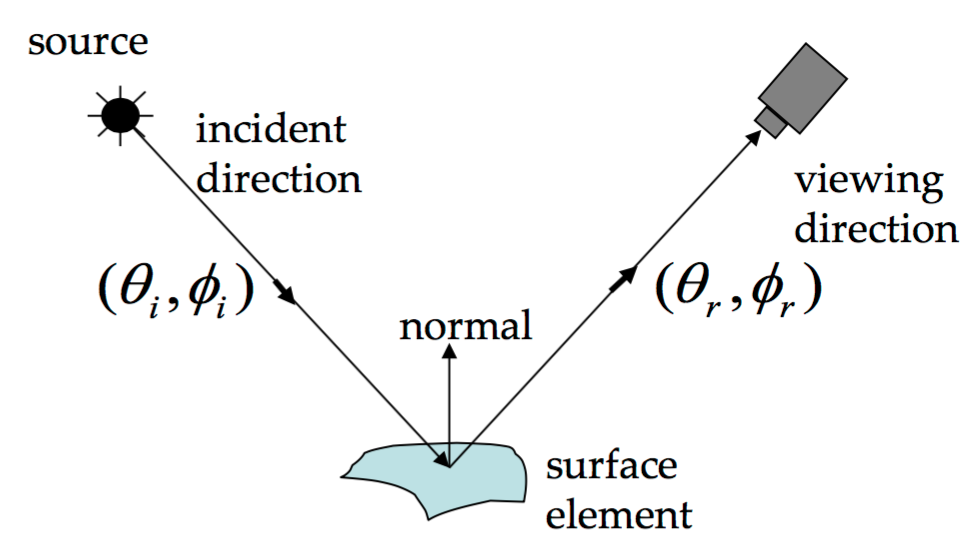
\includegraphics[width=0.5\textwidth]{model/brdf}
\caption{Surface reflection, image courtesy of Srinivasa Narasimhan}
\end{figure}

$\mathbf{E^{surface}(\theta_i, \phi_i)}$: irradiance at surface in direction $(\theta_i, \phi_i)$.

$\mathbf{L^{surface}(\theta_r, \phi_r)}$: irradiance at surface in direction $(\theta_r, \phi_r)$.

\textbf{Definition (BRDF)} the ratio of the radiance of the outgoing direction to the incident irradiance, \ie $f(\theta_i, \phi_i, \theta_r, \phi_r)=\frac{E^{surface}(\theta_i, \phi_i)}{L^{surface}(\theta_r, \phi_r)}$.

\textbf{Diffuse Albedo} or surface lightness is the proportion of incident light that is reflected by the surface. It should be noted that albedo is not an intrinsic property of a surface. Instead, for any surface, the albedo depends on the spectral and angular distributions of the incident light. 

The reflectance of light is dependent on the spectrum of the light, which means that the reflectance of the light is dependent on the light frequency, see Figure~\ref{fig:alb_freq}. We consider the reflectance across all spectrum, meaning only intensity albedo is considered.
\begin{figure}[h]
\centering
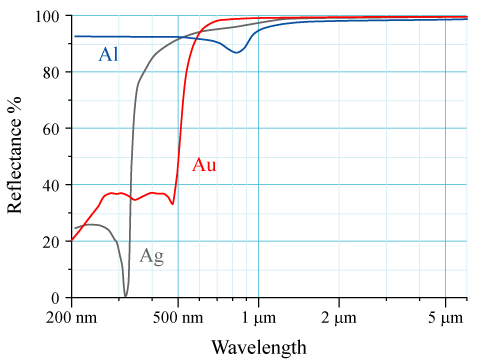
\includegraphics[width=0.5\textwidth]{model/reflectance_frequency}
\label{fig:alb_freq}
\caption{Spectral reflectance curves for aluminium (Al), silver (Ag), and gold (Au) metal mirrors at normal incidence.}
\end{figure}

The reflectance of light also depends on the incident direction. Specifically, light that lands on a surface at a grazing angle will be much more likely to reflect, see Figure~\ref{fig:alb_ang}. We take into account the Fresnel effect in the synthetic stage, thus we consider the albedo with small incident angle.
\begin{figure}[h]
\centering
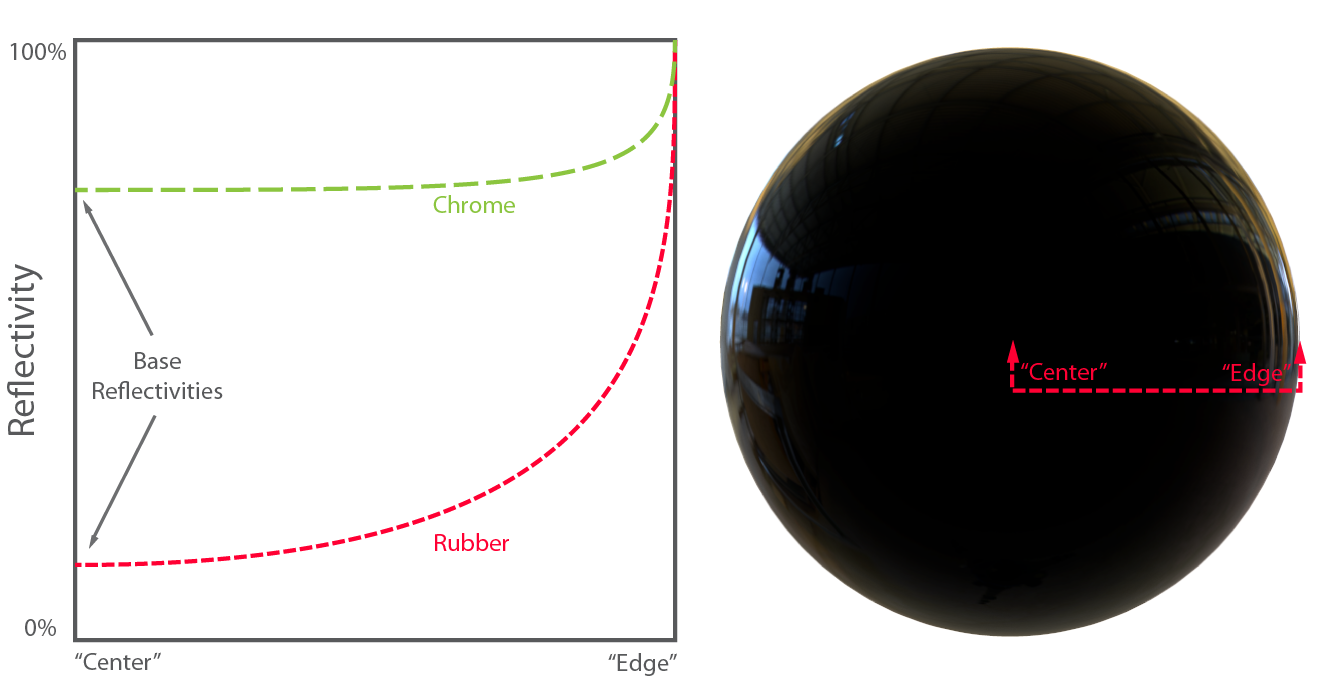
\includegraphics[width=0.5\textwidth]{model/reflectance_angle}
\label{fig:alb_ang}
% \caption{Spectral reflectance curves for aluminium (Al), silver (Ag), and gold (Au) metal mirrors at normal incidence.}
\end{figure}

It ranges from `black' to `white' in the grey scale axis. Colour is a superset intensity, which takes account into the spectral composition of light. Both terms depend on illumination, surface normal, surface reflectance, and viewing direction.

In order to understand the contributing factor of pixel intensity/colour, we need a in-depth understanding of reflection, \ie how light is reflected off of a surface patch, and the relation between incident light and intensity value.

\textbf{Specular} surfaces reflect light in almost a single direction when the microscopic surface irregularities is small compared to light wavelength, and no subsurface scattering present~\cite{nayar1989surface}. Unlike diffuse reflections, which we experience the lightness and colour of an object, specular reflections carry information about the structure, intensity, and spectral content of the illumination field. In other word, specular reflections are simply images of the environment, or the illumination field, distorted by the geometry of the reflecting surface. See Figure~\ref{fig:lake_spec}, the image no long reflect the original colour of the surface (red), instead it shows a distorted image of the environment. A purely specular surface is a mirror. Purely specular surfaces are rare in nature. Most natural materials exhibit a mix of specular and diffuse reflection. Variations in microscopic surface geometry can cause specular reflections to be scattered, blurring the image of the environment in an amount proportional to surface roughness.
\begin{figure}[h]
\centering
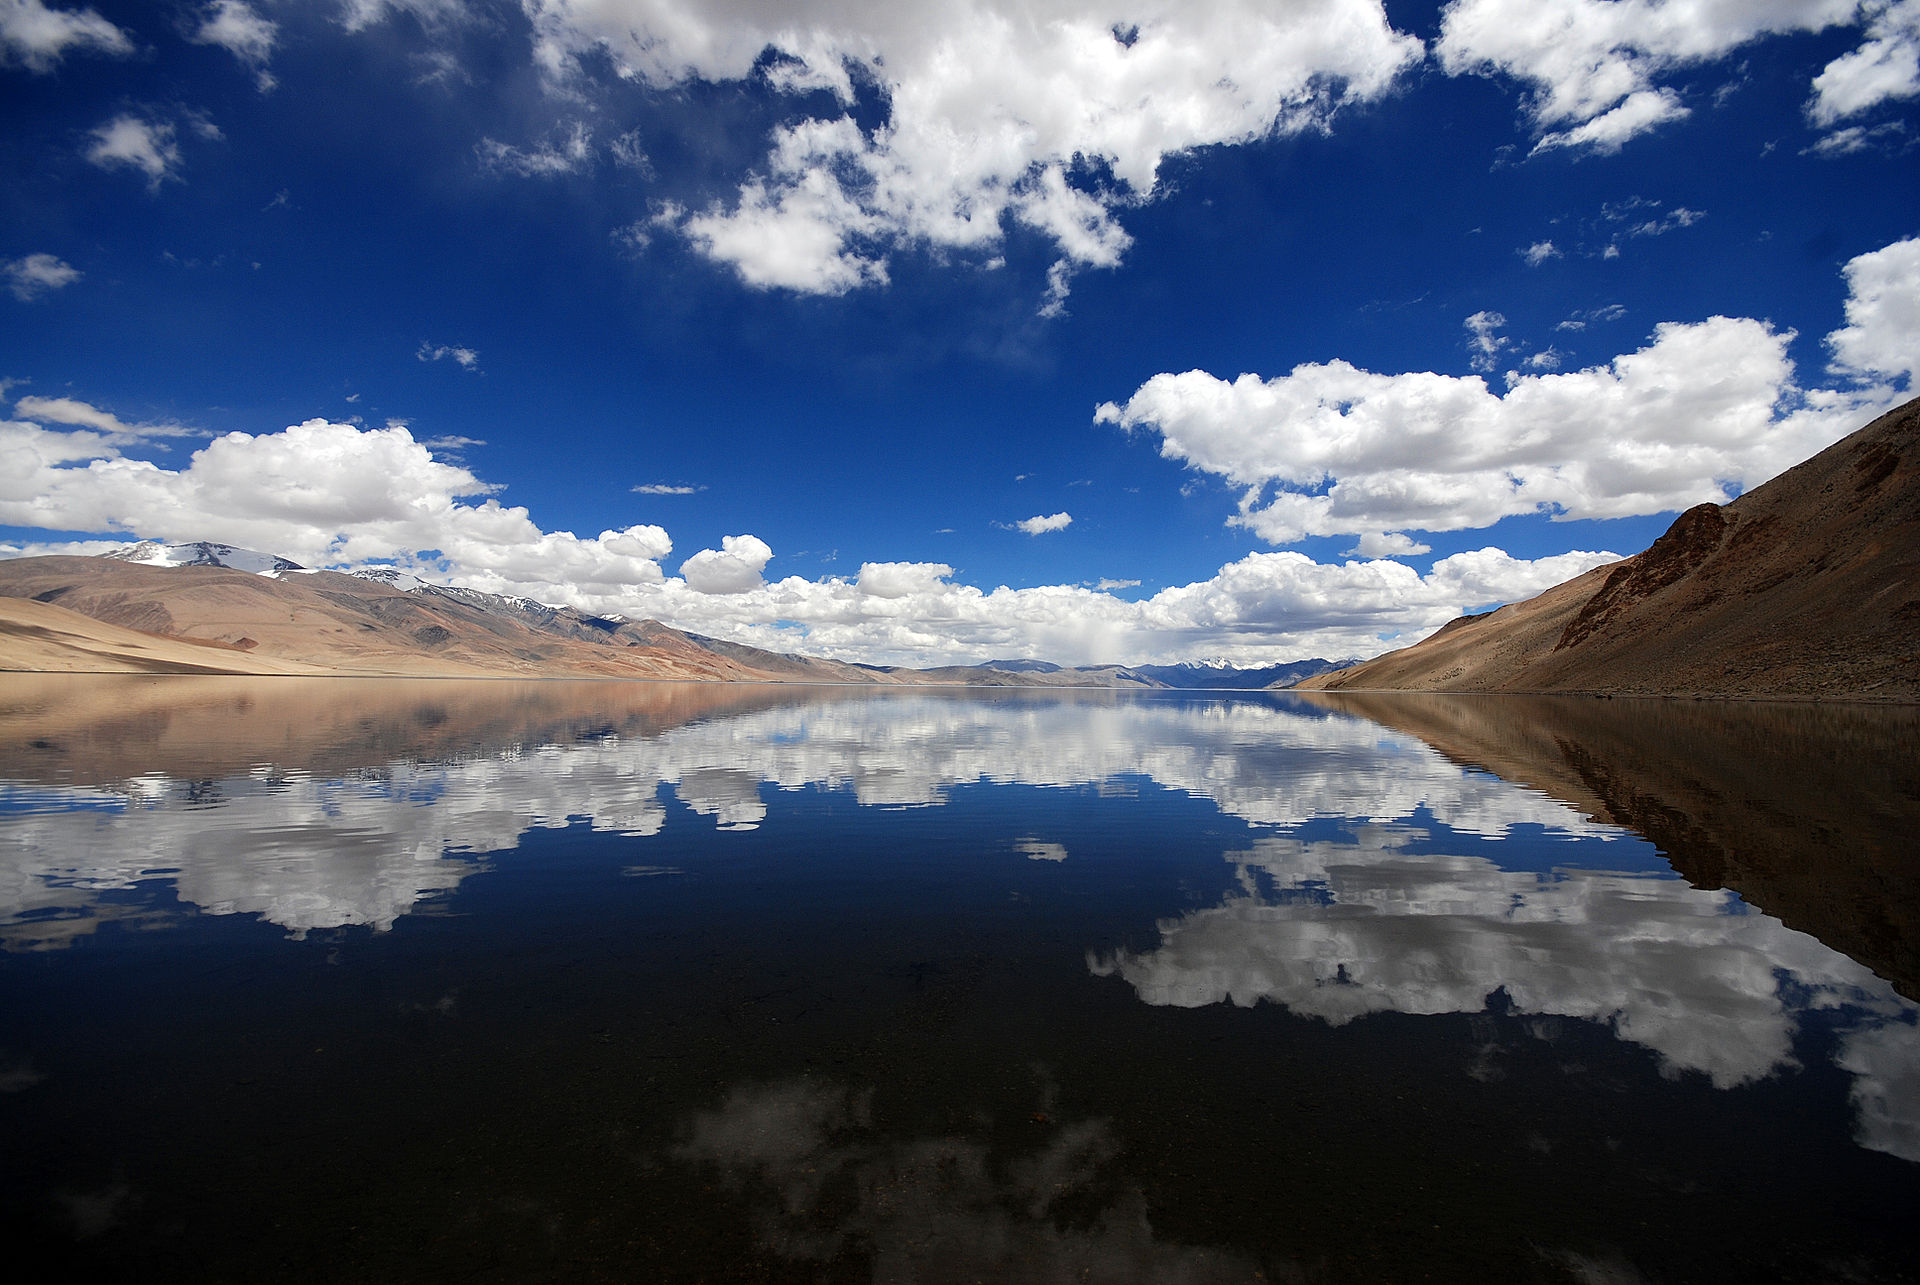
\includegraphics[width=0.5\textwidth]{model/lake_spec}
\label{fig:lake_spec}
\end{figure}

Another observation is that from the image changes as the viewer changes. This can be derived directly from specular reflection, which make stereo correspondence searching extremely challenging.

\textbf{Roughness}, which is characterized as the microscopic shape characteristics of the surface, contributes to the way in which light is reflected off of a surface. A smooth surface may reflect incident light in a single direction, while a rough surface may scatter the light in various directions. We need prior knowledge of the microscopic surface irregularities, or a model of the surface to determine the reflection of incident light.

The possible surface models are divided into 2 categories: surface with exactly known profiles and surfaces with random irregularities. An exact profile may be determined by measuring the height at each point on the surface by means of a sensor such as the stylus profilometer. This method is cumbersome and impractical. Hence, it’s more reasonable to model the surface as a random process, where it is described by a statistical distribution of either its height above a certain mean level, or its slope w.r.t its mean (macroscopic) slope. The section only discusses these second statistical approach.

% \textit{Height Distribution Model} The height coordinate of the surface is expressed as random function of the coordinates $x$ and $y$.
% \begin{figure}[h]
% \centering
% \includegraphics[width=0.5\textwidth]{model/surface_representation_1}
% \caption{Surface height distribution model}
% \end{figure}

% The shape of the surface is determined by the probability distribution of $h$. For instance, let $h$ be normally distributed, with mean value $\bar{h}=0$ and standard deviation $\sigma_h$. Then, the distribution of $h$ is given by:
% $$
% p_h(h)=\frac{1}{\sqrt{2\pi}\sigma_h}e^{-\frac{h^2}{2\sigma_h^2}}
% $$

% The $\sigma_h$ is the root-mean-square of $h$ and represents the roughness of the surface. The surface is not uniquely described by the distribution of $h$, as it does not tell us anything about the distance between the hills and valleys of the surface.

% The surfaces below have the same height distribution function, i.e., the same mean value and standard deviation. However, they don't resemble each other in appearance.
% \begin{figure}[h]
% \centering
% \includegraphics[width=8cm]{model/same_mean_sd}
% \caption{Surface height distribution model}
% \end{figure}

% An autocorrelation coefficient $C(\tau)$ is introduced, that determines the correlation (or lack of independence) between the random values assumed by the height $h$ at two surface points $(x_1, y_1)$ and $(x_2, y_2)$, separated by a distance $\tau$. The autocorrelation coefficient can be:
% $$
% C(\tau)=e^{-\frac{\tau^2}{T^2}}
% $$

% where $T$ is the *correlation distance*. Therefore, the above surfaces have small and large correlation distances respectively.

\textit{Slope Distribution Model} We can also think of a surface as a collection of planar micro-facets.
\begin{figure}[h]
\centering
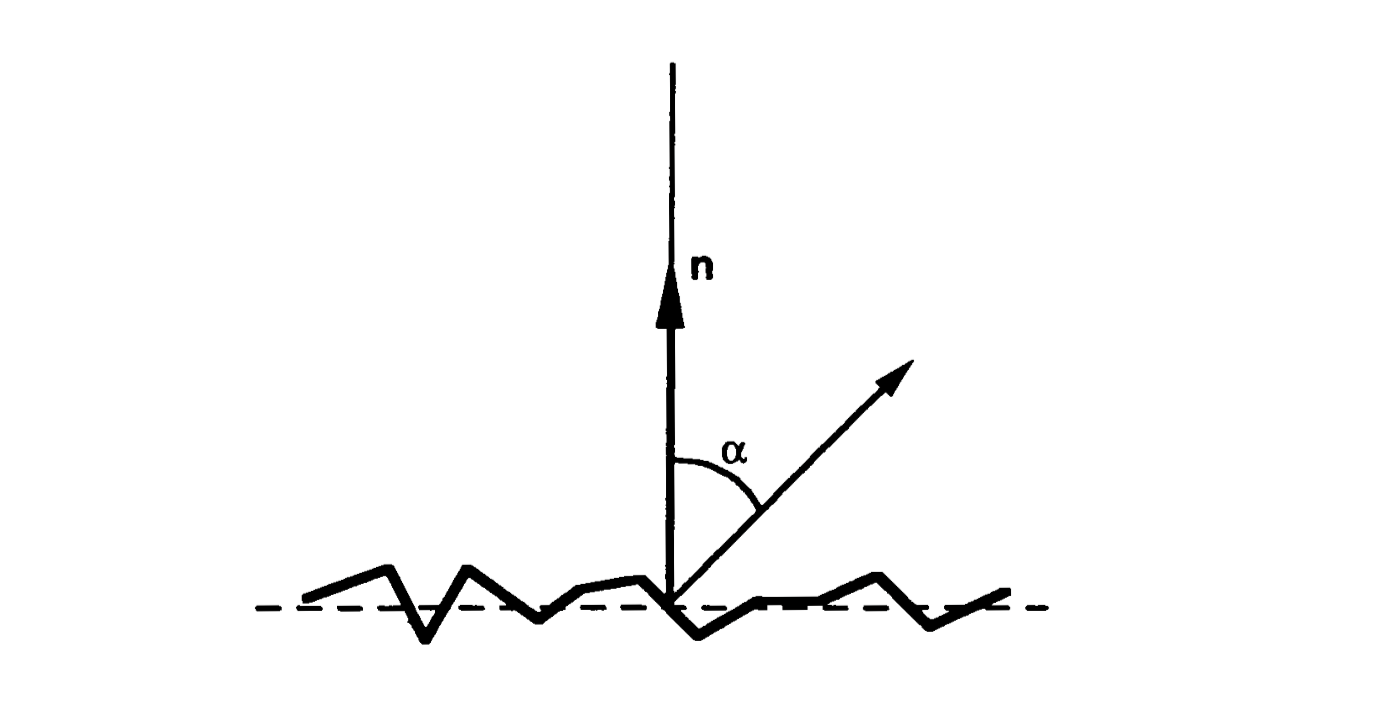
\includegraphics[width=0.7\textwidth]{model/surface_representation_2}
\caption{Surface Slope Distribution Model}
\end{figure}

A large set of micro-facets constitutes an infinitesimal surface patch that has a mean surface orientation $\vec{n}$. Each micro-facet has its own orientation, which may deviate from the mean surface orientation by an angle $\alpha$. 

We will use the parameter $\alpha$ to represent the slope of individual facets. Surfaces can be modeled by a statistical distribution of the micro-facet slopes. If the surface is isotropic, the probability distribution of the micro-facet slopes can be assumed to be rotationally symmetric w.r.t the mean surface normal $\vec{n}$.  Therefore, facet slopes can be described by a one-dimensional probability distribution function. For instance, the surface may be modeled by assuming a normal distribution for the facet slope $\alpha$, with mean value $\bar{\alpha}=0$ and standard deviation $\sigma_\alpha$:
$$
p_\alpha(\alpha)=\frac{1}{\sqrt{2\pi}\sigma_\alpha}e^{-\frac{\alpha^2}{2\sigma_\alpha^2}}
$$

The surface model is determined by a single parameter $\sigma_\alpha$, and larger $\sigma_\alpha$ can be used to model rougher surfaces. While autocorrelation coefficient is important, the concept of slope correlation is more difficult to interpret and is not that useful in the generation of surface, which results in a weaker model compared to the height model. However, slope distribution model is popular in the analysis of surface reflection, as the scattering of light rays is dependent on the local slope of the surface and not the local height of the surface.

% surface roughness will affect the fresnel and specularity

% \subsubsection{Sub-surface Scattering}
% Sub-surface scattering can also cause diffuse reflection.

\textbf{Concavity} can cause self-shadow or inter-reflection effect, which can severely impede the accuracy of intensity based algorithms. Since concavity is not shown in the silhouette image, methods that utilize silhouette information may also fail to reconstruct concavities. Concavity is measured by \textit{surface curvature}.

\subsubsection{Silhouette}
\textbf{Concavity} is not shown in the silhouette image, thus methods that utilize silhouette information may fail to reconstruct concavities. Concavity is measured by \textit{surface curvature}.

\section{Expression}
\label{sec:3DRecon_Exp}
Now with the proposed definition and representation of 3D reconstruction problem, we can express some existing 3D reconstruction algorithms under this framework.
\begin{figure}[h!]
\centering
\begin{tabular}{cc}
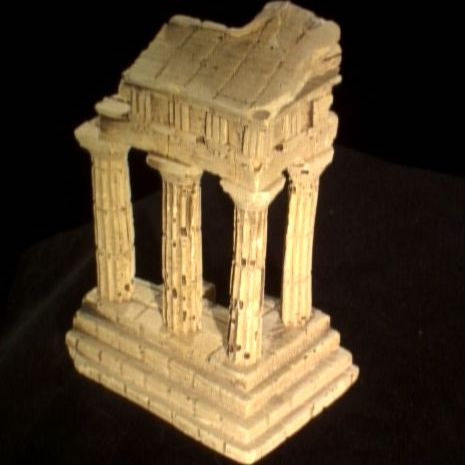
\includegraphics[width=0.5\textwidth]{model/temple}&
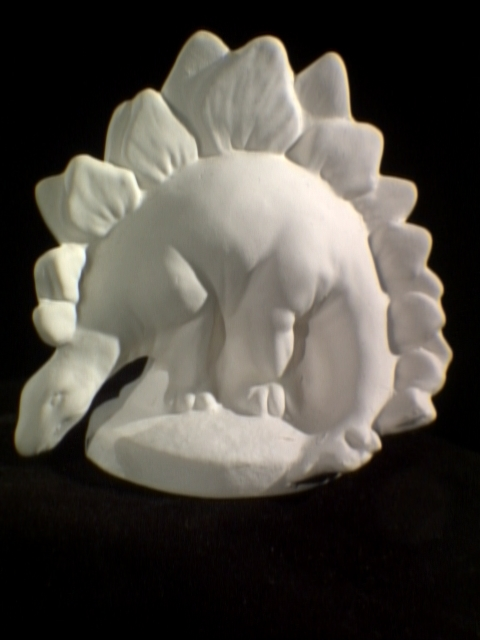
\includegraphics[width=0.5\textwidth]{model/dino}\\
Temple & Dino\\
\end{tabular}
\caption{Image of ``temple'' and ``dino'' datasets}
\label{fig:temple_dino}
\end{figure}

We start with the middlebury dataset. For the ``temple'' dataset, the expression of the reconstruction problem is shown in table~\ref{tab:exp_temple}.
\begin{table}[h]
  \centering
  \begin{tabular}{*{5}{c}}
  \hline
  Texture coverage & Albedo & Specular & Roughness & Concavity\\
  \hline
  0.8 & 0.8 & 0.2 & 0.8 & 0.5\\
  \hline
  \end{tabular}
  \label{tab:exp_temple}
  \caption{Expression of the reconstruction problem for the ``temple'' dataset.}
\end{table}

The second example is the ``dino'' dataset.
\begin{table}[h]
  \centering
  \begin{tabular}{*{5}{c}}
  \hline
  Texture coverage & Albedo & Specular & Roughness & Concavity\\
  \hline
  0.2 & 0.8 & 0.2 & 0.2 & 0.2\\
  \hline
  \end{tabular}
  \label{tab:exp_dino}
  \caption{Expression of the reconstruction problem for the ``dino'' dataset.}
\end{table}

The third example is ``cat'' dataset from the ``DiLiGenT'' photometric stereo dataset, see Figure~\ref{fig:cat_statue}.
\begin{figure}[h!]
\centering
\begin{tabular}{cc}
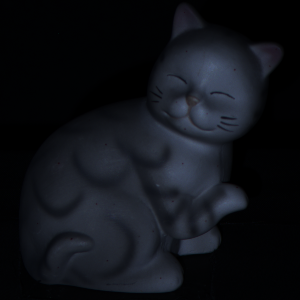
\includegraphics[width=0.5\textwidth]{model/cat}&
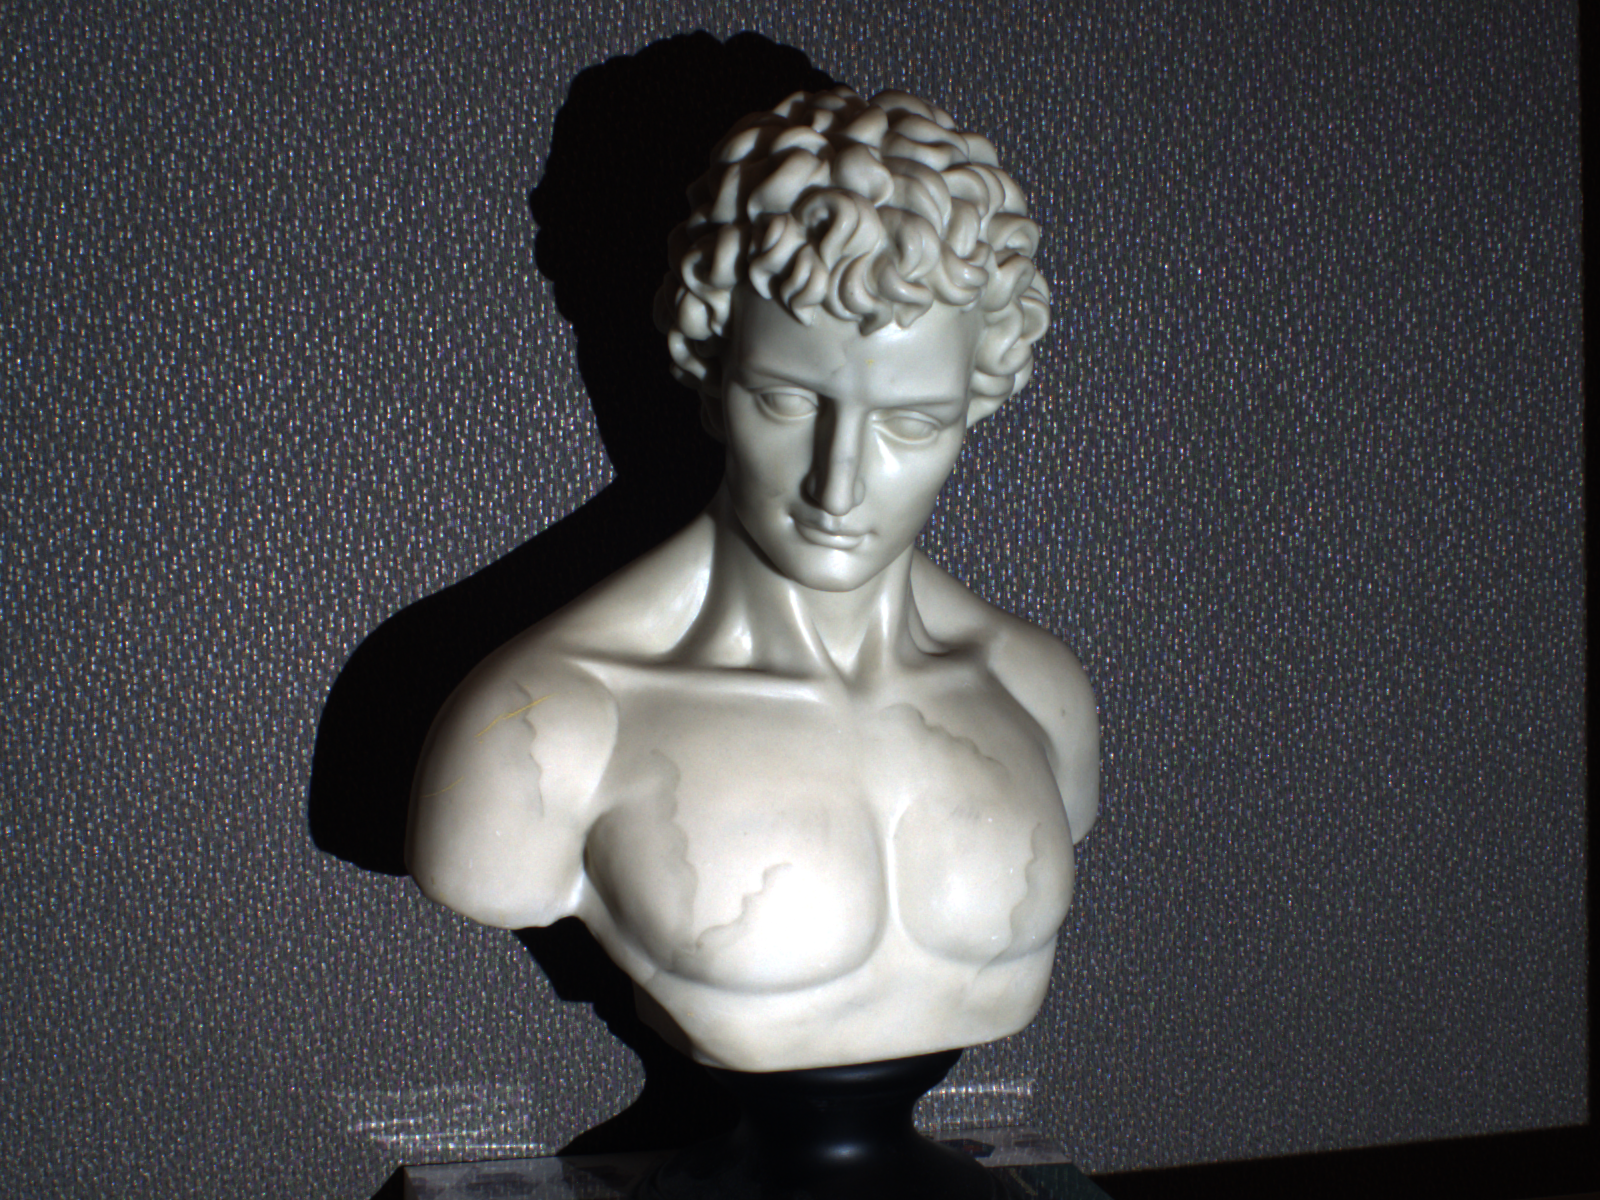
\includegraphics[width=0.5\textwidth]{model/statue}\\
Cat & Statue\\
\end{tabular}
\caption{Image of ``cat'' and ``statue'' datasets}
\label{fig:cat_statue}
\end{figure}

\begin{table}[h]
  \centering
  \begin{tabular}{*{5}{c}}
  \hline
  Texture coverage & Albedo & Specular & Roughness & Concavity\\
  \hline
  0.2 & 0.8 & 0.2 & 0.2 & 0.2\\
  \hline
  \end{tabular}
  \label{tab:exp_cat}
  \caption{Expression of the reconstruction problem for the ``cat'' dataset.}
\end{table}

The last example is the ``statue'' dataset from the 
\begin{table}[h]
  \centering
  \begin{tabular}{*{5}{c}}
  \hline
  Texture coverage & Albedo & Specular & Roughness & Concavity\\
  \hline
  0.2 & 0.8 & 0.2 & 0.2 & 0.2\\
  \hline
  \end{tabular}
  \label{tab:exp_statue}
  \caption{Expression of the reconstruction problem for the ``statue'' dataset.}
\end{table}
%% The following is a directive for TeXShop to indicate the main file
%%!TEX root = diss.tex

\chapter{A benchmark of 3D Reconstruction Techniques}
\label{ch:3DRecon_Benchmark}
Current existing 3D benchmarks all focus on one specific class of algorithms, for example, the Middlebury dataset is targeted to MVS algorithms, and the `DiLiGenT' dataset is for Photometric Stereo algorithms. This makes them suitable only to the evaluation of algorithms within the same category. There is no dataset that evaluates 3D reconstruction across differ categories, let alone one that covers a range of properties and their combinations. The reasons for the lack of such dataset is: 1). it's tedious to create a real-world dataset for a specific category of algorithm, it would be more challenging to create datasets for a range of categories with the ground truth; 2). it's practically impossible to make one property (\eg, noise level, lighting configuration, material, etc) varied while fixing the other in order to conduct a thorough evaluation.

We propose a synthetic but realistic (physically-based) benchmark for evaluation of 3D reconstruction algorithms. Each benchmark dataset includes a collection of images of a scene under different material or lighting conditions, together with ground-truth point cloud, and surface normals. The datasets are organized into `depend\_check' and `training' in which one property of the object is varied while others are kept constant.

\section{Synthetic setup}
We use the physically-based renderer Cycles in Blender. For each technique, the configuration of the camera remains fixed. The image resolution is 1280$\times$720. For MVS, there are five rings of camera, of which the elevation angle is 15$^\circ$, 30$^\circ$, 45$^\circ$, 60$^\circ$, 90$^\circ$. The angle between two neighbouring camera in the first four rings is 30$^\circ$, 30$^\circ$, 45$^\circ$, and 45$^\circ$. Thus there are in total $12+12+8+8+1=41$ cameras.

For photometric stereo, according to \cite{Berkiten2016rgbn}, increasing the number of images is only important up to a point, the experimental results showed that most algorithms reaches to optimum when 15 images are used. To make a balance between algorithm performance and rendering time, we use 25 light sources, which are distributed on four different rings with elevation angle of 90$^\circ$, 85$^\circ$, 60$^\circ$, and 45$^\circ$. The azimuth angle between two neighbouring light sources is 45$^\circ$.

For the structured light, the baseline angle between the camera and the projector is 10$^\circ$, and only one camera is used, thus only a portion of the object is invisible. The resolution of the projector is 1024$\times$768, thus 10 Gray code patterns are needed. To counter the effect of inter-reflection, each pattern and its inverse are projected, which makes it less sensitive to scattered light.

\section{Structure of Datasets}
Due to the number of properties and number of levels for each property, it would be unrealistic to render all the combinations of properties. For if we have $N$ properties and each is discretized into $L$ levels, the number of different combinations is $L^N$, and for each combination, there are in total $41+25+42=108$ images to render. Therefore, we take another approach: 1). first we investigate the dependency between any two properties, if these two properties are independent, there is no need to render all their combinations whereas it's necessary to do so if they are dependent; 2). render all the combinations for dependent properties.

The camera/projector intrinsic and extrinsic parameters are computed directly from the positions and orientations of the synthetic setup, and the ground truth including the 3D model and normal map are generated directly from Blender.

\section{Selected methods}
We have selected three algorithms: the PMVS proposed by~\citeauthor{furukawa2010accurate} ($C_n-S-T-P-P$), the example-based photometric stereo proposed by~\citeauthor{hertzmann2005example} ($C_1L_n-T-I-MDS-N$), and the Gray-encoded structured light technique ($C_1P-T-I-B-P$).

\section{Evaluation metrics}
We use the metric proposed by \citeauthor{seitz2006comparison} to evaluate MVS and SL. More specifically, we compute the accuracy and completeness of the reconstruction. For accuracy, the distance between the points in the reconstruction $R$ and the nearest points on ground truth $G$ is computed, and the distance $d$ such that $X\%$ of the points on $R$ are within distance $d$ of $G$ is considered as accuracy. Thus the lower the accuracy value, the better the reconstruction result. The completeness measures the fraction of points of $G$ that are within an allowable distance $d$ of $R$.

For photometric stereo, we employ another evaluation criteria, which is based on the statistics of angular error. For each pixel, the angular error is calculated as $arccos$($n_g^T n$) in degrees, where $n_g$ and $n$ are ground truth and estimated normals respectively. In addition to the mean angular error, we also calculate the minimum, maximum, median, the first quartile, and the third quartile of angular errors for each estimated normal map.

\section{Dependency Check}
Part of the difficulty in establishing a comprehensive set of experiments for such an evaluation is the large variability of shapes and material properties.

\subsection{$C_n-S-T-P-P$}
We evaluate the performance of MVS in terms of accuracy and completeness under varied combination of properties.
\begin{table}[h]
  \centering
  \begin{tabular}{l*{5}{c}}
  \hline
  \textbf{Property} & Texture coverage & Albedo & Specular/Diffuse ratio & Roughness\\
  \hline
  \textit{Value} & 0.2-0.8 & 0.2-0.8 & 0.0 & 0.0\\
                 & 0.2-0.8 & 1 & 0.2-0.8 & 0.0\\
                 & 0.2-0.8 & 1 & 0.0 & 0.2-0.8\\
                 & 1.0 & 0.2-0.8 & 0.2-0.8 & 0.0\\
                 & 1.0 & 0.2-0.8 & 0.0 & 0.2-0.8\\
                 & 1.0 & 1.0 & 0.2-0.8 & 0.2-0.8\\
  \hline
  \end{tabular}
  \caption{Parameter of MVS with varied texture and albedo}
\end{table}

\textbf{(a) Texture and Albedo} 
For a fixed texture, the accuracy and completeness doesn't change much as the albedo changes, which shows that the influence of the texture on the performance is not impacted by albedo.

For a fixed albedo, the accuracy remains almost the same and completeness goes up a little bit as texture level goes up, which demonstrates that the texture level has a larger influence on the completeness instead of the accuracy, which is consistent with the real-world data.

\textbf{(b) Texture and Specularity} 
For a fixed texture, as the specularity goes up, the accuracy value of MVS goes up, and the completeness goes down, meaning the reconstruction gets worse as specularity goes up.

For a fixed specularity, the accuracy goes down as the texture level goes up, and the completeness goes up as the texture goes up, which means the reconstruction gets more accurate and more complete, which is consistent with the results obtained from real-world data. But for lower specularity, the impact of texture is more substantial, thus these two properties are dependent to each other.

\textbf{(c) Texture and Roughness} 
For a fixed texture, the accuracy and completeness doesn't change much as the roughness changes, which shows that the influence of the texture on the performance is not impacted by roughness.

For a fixed roughness, the accuracy remain almost the same and completeness goes up as texture level goes up, which demonstrate again that the texture level has a larger influence on the completeness instead of the accuracy, which is consistent with the real-world data.

\textbf{(d) Albedo and Specularity} 
For a fixed albedo, the accuracy increases and the completeness decreases as the specularity increases, which demonstrates the effect of specularity. Since we're using a physical-based rendering engine (PBR), the diffuse decrease as the specularity increases.

for a fixed specularity, the accuracy increase and the completeness decreases as the albedo increases, but this effect is more noticeable for lower albedo, highly specular surface, which shows that albedo and specularity are two dependent properties.

\textbf{(e) Albedo and Roughness} 
For a fixed albedo, the accuracy and completeness remain almost the same as the roughness changes.

For a fixed roughness, the accuracy and completeness remain also almost the same as the albedo changes, which is also consistent with the real-world scenario. Thus these two properties are independent to each other.

\textbf{(f) Specularity and Roughness} 
For a fixed specularity, the accuracy and consistency doesn't change much as the roughness changes especially when specularity is low.

For a fixed roughness, the accuracy value increases and completeness value decreases, which again shows that the specularity can affect the MVS.

Therefore, specularity has an impact on MVS, but its effect won't be interfered by roughness, thus those two properties are independent.

\textbf{Conclusion} the properties that have an effect on the MVS are: texture, albedo, and specularity. Therefore, we will only consider these three properties for all forthcoming discussion of MVS.

\begin{figure}[h!]
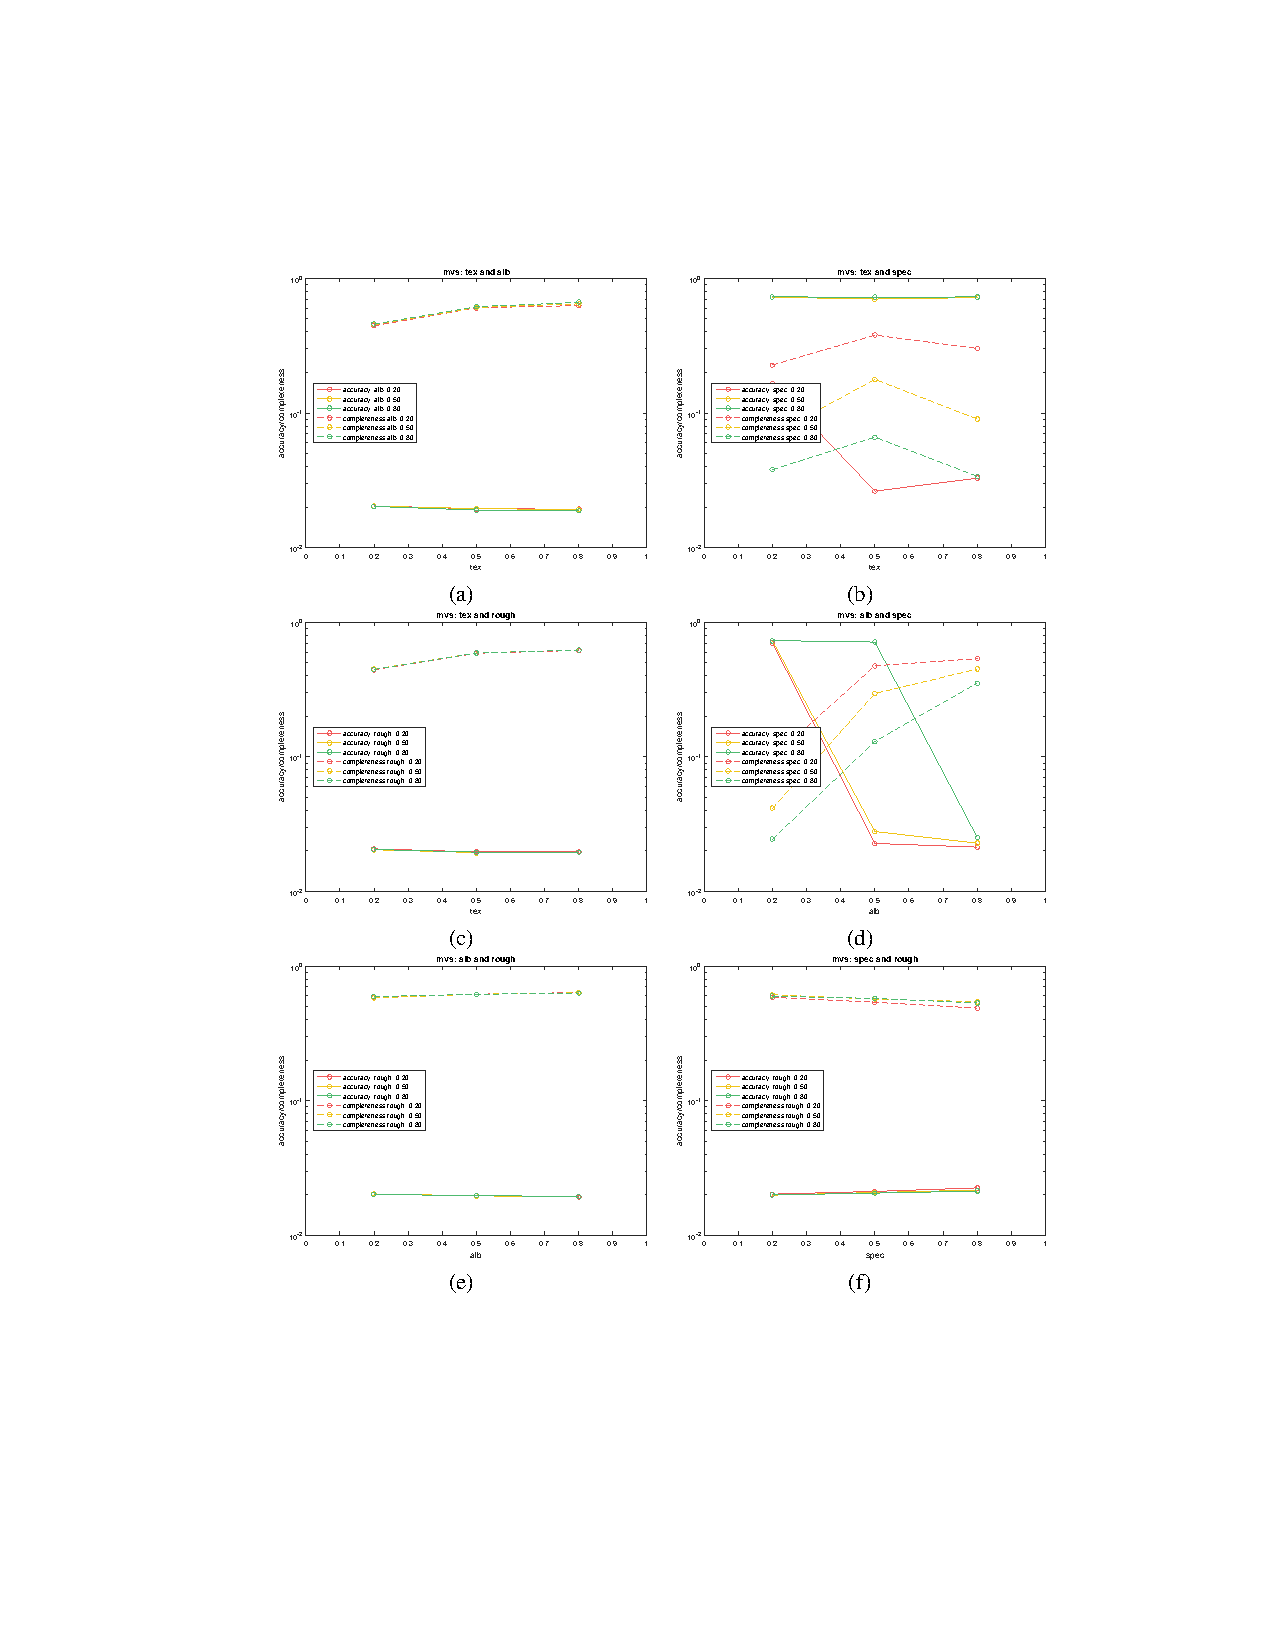
\includegraphics[width=\textwidth]{training/depend_check_mvs}
\caption{Performance of MVS with varied properties}
\label{fig:depend_check_mvs}
\end{figure}

\subsection{$C_1L_n-T-I-MDS-N$}
We evaluate the performance of PS in terms of angle difference under varied combinations of properties. The statistical measures that we used include median, mean, first and third quartile. We investigate two properties at a time.

\begin{table}[h]
  \centering
  \begin{tabular}{l*{5}{c}}
  \hline
  \textbf{Property} & Texture coverage & Albedo & Specular/Diffuse ratio & Roughness\\
  \hline
  \textit{Value} & 0.2-0.8 & 0.2-0.8 & 0.0 & 0.0\\
                 & 0.2-0.8 & 1 & 0.2-0.8 & 0.0\\
                 & 0.2-0.8 & 1 & 0.0 & 0.2-0.8\\
                 & 0.0 & 0.2-0.8 & 0.2-0.8 & 0.0\\
                 & 0.0 & 0.2-0.8 & 0.0 & 0.2-0.8\\
                 & 0.0 & 1.0 & 0.2-0.8 & 0.2-0.8\\
  \hline
  \end{tabular}
  \caption{Parameter of PS with varied properties}
\end{table}

\textbf{(a) Texture and Albedo} 
For a fixed texture, as the albedo level goes up, all the statistic measures go down, which means that the reconstruction gets better as albedo level goes up, which is consistent to the real-world scenario.

For a fixed albedo, the angle difference doesn't change much as the texture level changes, which shows that texture doesn't interfere with albedo, and these two properties are thus independent.

\textbf{(b) Texture and Specularity} 
For a fixed texture, as the specularity goes up, all the statistic measures go up, which means that the reconstruction gets worse as specularity level goes up, which is consistent to the real-world scenario.

For a fixed specularity, the angle difference doesn't change much as the texture level changes, which shows that texture doesn't interfere with specularity, and these two properties are independent.

\textbf{(c) Texture and Roughness} 
For a fixed texture, as the roughness goes up, all the statistic measures go down, which means that the reconstruction gets better as roughness level goes up.

For a fixed roughness, the angle difference doesn't change much as the texture level changes, which shows that texture doesn't interfere with roughness, and these two properties are independent.

\textbf{(d) Albedo and Specularity} 
We're using a physically-based renderer, thus the higher the specularity, the less the diffusion would be. Thus rising specularity would `darken' the diffuse areas.

For a fixed albedo, the angle difference goes up as the specularity rises, which demonstrate that PS can't deal with high specularity, and it's worse for lower albedo surfaces than that for the higher albedo surfaces, which is consistent to real-world scenario.

For a fixed specularity, the angle difference goes down as the albedo rises, which is consistent to the real-world scenario since high albedo would make the intensity variation more distinctive.

\textbf{(e) Albedo and Roughness} 
For a fixed albedo, as the roughness goes up, all the statistic measures go down, which means that the reconstruction gets better as roughness level goes up.

For a fixed roughness, the angle difference also goes down as the albedo level goes up, which shows that albedo does interfere with roughness, and these two properties are dependent.

\textbf{(f) Specularity and Roughness}
For a fixed specularity, if the specularity is lower, the effect of roughness is less noticeable, whereas if the specularity is higher, the effect of roughness becomes more substantial. We've also noticed a `peculiar' case when roughness is 0.5, it makes the reconstruction worse, which is counter-intuitive. However, we argue that it's because the roughness effect is not strong enough to cancel out the specularity, thus causing a much larger area of `blurred' specularity, which makes the reconstruction worse. This effect is also demonstrated in the training stage, see Figure~\ref{fig:ps_outlier} for some visual examples.

For a fixed roughness, increasing the specularity would make the angle difference worse. The effect is less substantial when the roughness is higher or when the specularity is lower.

Therefore, the specularity and roughness cancels each other's effect, thus they are dependent properties, which is consistent to visual inspection.

\textbf{Conclusion} the properties that have an effect on the PS are: albedo, specularity, and roughness. Therefore, we will only consider these three properties for all forthcoming discussion of PS.

\begin{figure}[h!]
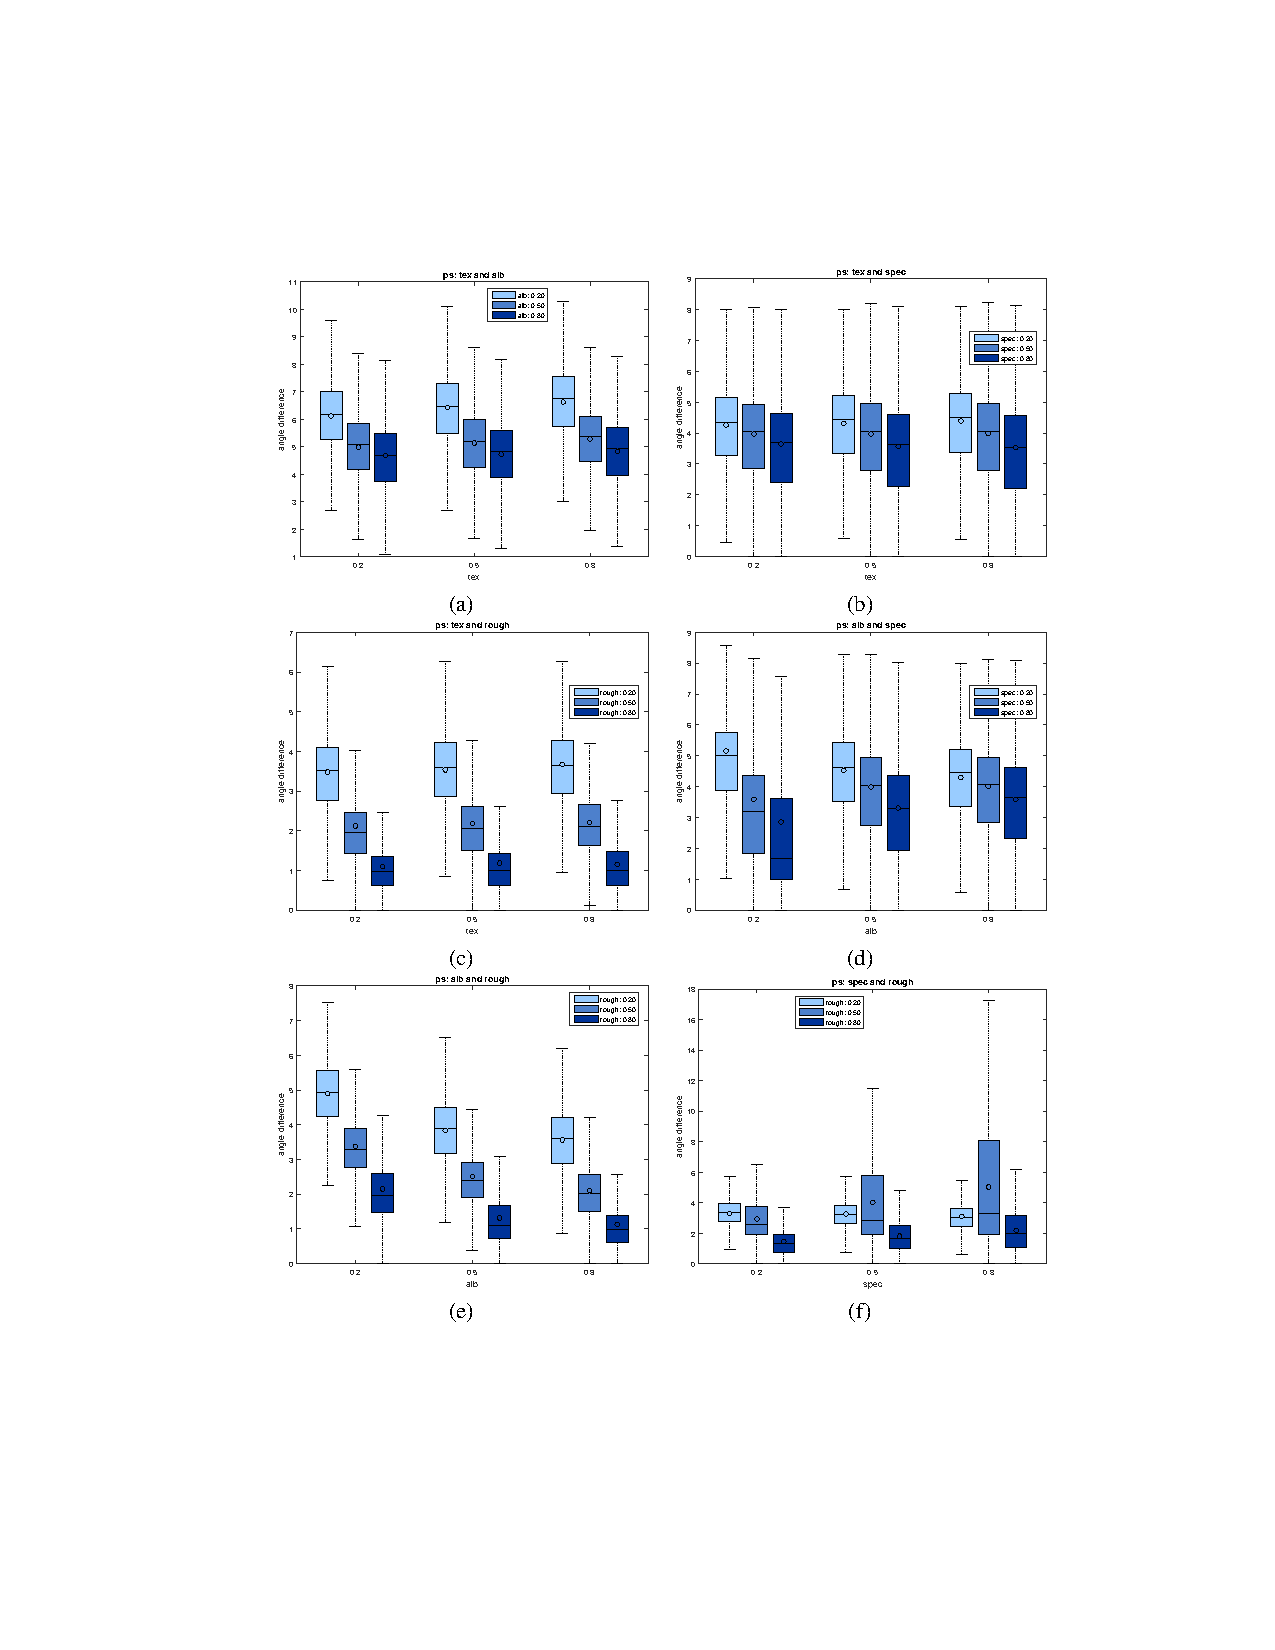
\includegraphics[width=\textwidth]{training/depend_check_ps}
\caption{Performance of PS with varied properties}
\label{fig:depend_check_ps}
\end{figure}

\subsection{$C_1P-T-I-B-P$}
We evaluate the performance of SL in terms of accuracy and completeness under varied combination of properties.

\begin{table}[h]
  \centering
  \begin{tabular}{l*{5}{c}}
  \hline
  \textbf{Property} & Texture coverage & Albedo & Specular/Diffuse ratio & Roughness\\
  \hline
  \textit{Value} & 0.2-0.8 & 0.2-0.8 & 0.0 & 0.0\\
                 & 0.2-0.8 & 1 & 0.2-0.8 & 0.0\\
                 & 0.2-0.8 & 1 & 0.0 & 0.2-0.8\\
                 & 0.0 & 0.2-0.8 & 0.2-0.8 & 0.0\\
                 & 0.0 & 0.2-0.8 & 0.0 & 0.2-0.8\\
                 & 0.0 & 1.0 & 0.2-0.8 & 0.2-0.8\\
  \hline
  \end{tabular}
  \caption{Parameter of SL with varied properties}
\end{table}

Our current implementation of SL projects column patterns and a row patterns, and compute depth values using images captured using these two kinds of patterns individually. A depth consistency checking step is performed to reject erreneous triangulations, thus the accuracy remains almost the same across all cases.

\textbf{(a) Texture and Albedo} 
For a fixed texture, as the albedo goes up, the accuracy value of SL remain almost the same, whereas the completeness goes up, meaning that the reconstruction gets more dense as albedo goes up, which is consistent to real-world scenario.

For a fixed albedo, the accuracy remains almost the same as the texture level goes up, and the completeness goes down a little as the texture goes up, which demonstrate the real-world observation that surface texture would interfere with some SL techniques.

\textbf{(b) Texture and Specularity} 
No substantial changes when either of the two properties changes.

\textbf{(c) Texture and Roughness} 
No substantial changes when either of the two properties changes.

\textbf{(d) Albedo and Specularity} 
For a fixed albedo, the completeness goes down as the specularity goes up for low albedo surface, this effect becomes less when the albedo increases. Thus these two properties are dependent

\textbf{(e) Albedo and Roughness} 
No substantial changes when either of the two properties changes.

\textbf{(f) Specularity and Roughness} 
No substantial changes when either of the two properties changes.

\textbf{Conclusion} the properties that have an effect on the SL are: texture, albedo, specularity. Therefore, we will only consider these three properties for all forthcoming discussion of SL.

\begin{figure}[h!]
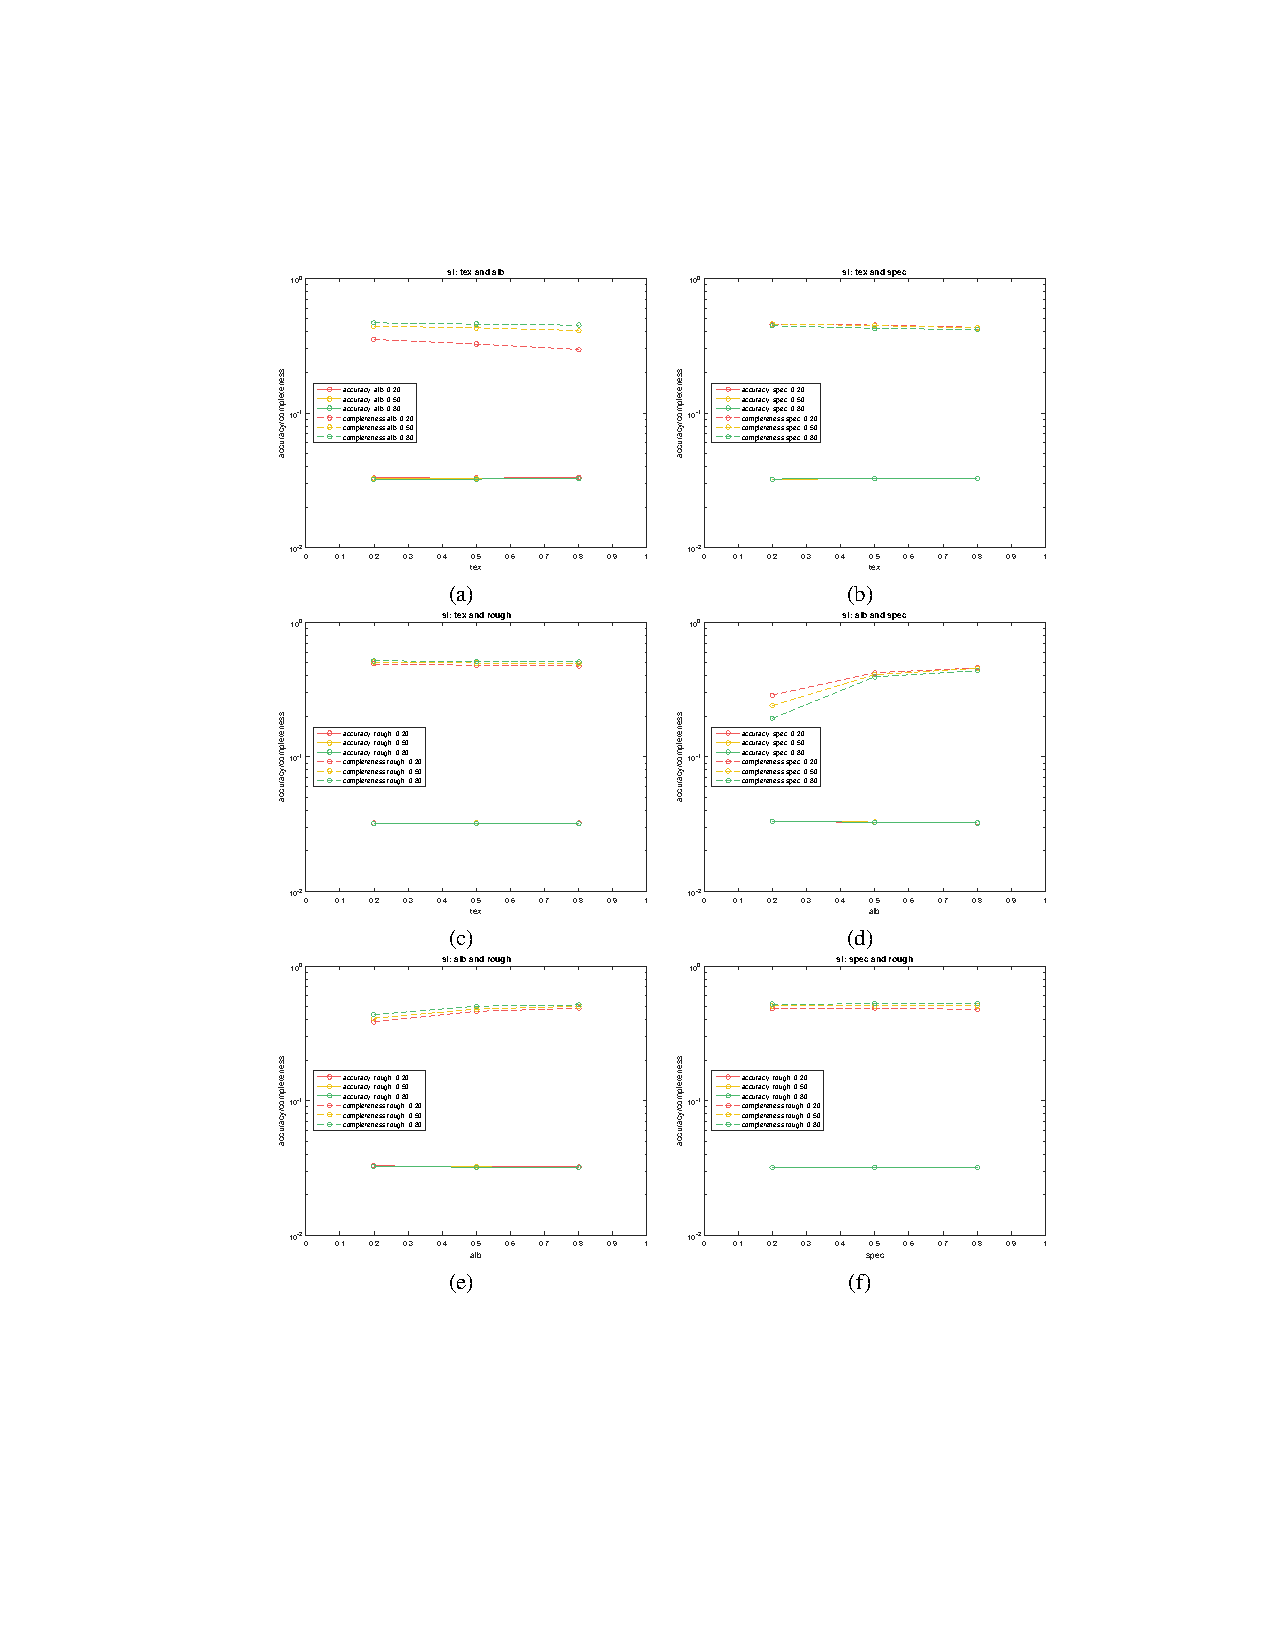
\includegraphics[width=\textwidth]{training/depend_check_sl}
\caption{Performance of SL with varied properties}
\label{fig:depend_check_sl}
\end{figure}

\section{Training}
For each technique, we generate the synthetic dataset using only the dependent properties, thus there are $L\times L\times L$ different combinations for each technique, where $L$ is the number of levels for each property. We show the performance of each technique w.r.t one property in Figure~\ref{fig:training}, note that column 2, 3 uses the exactly same data as column 1.

\begin{figure}[h!]
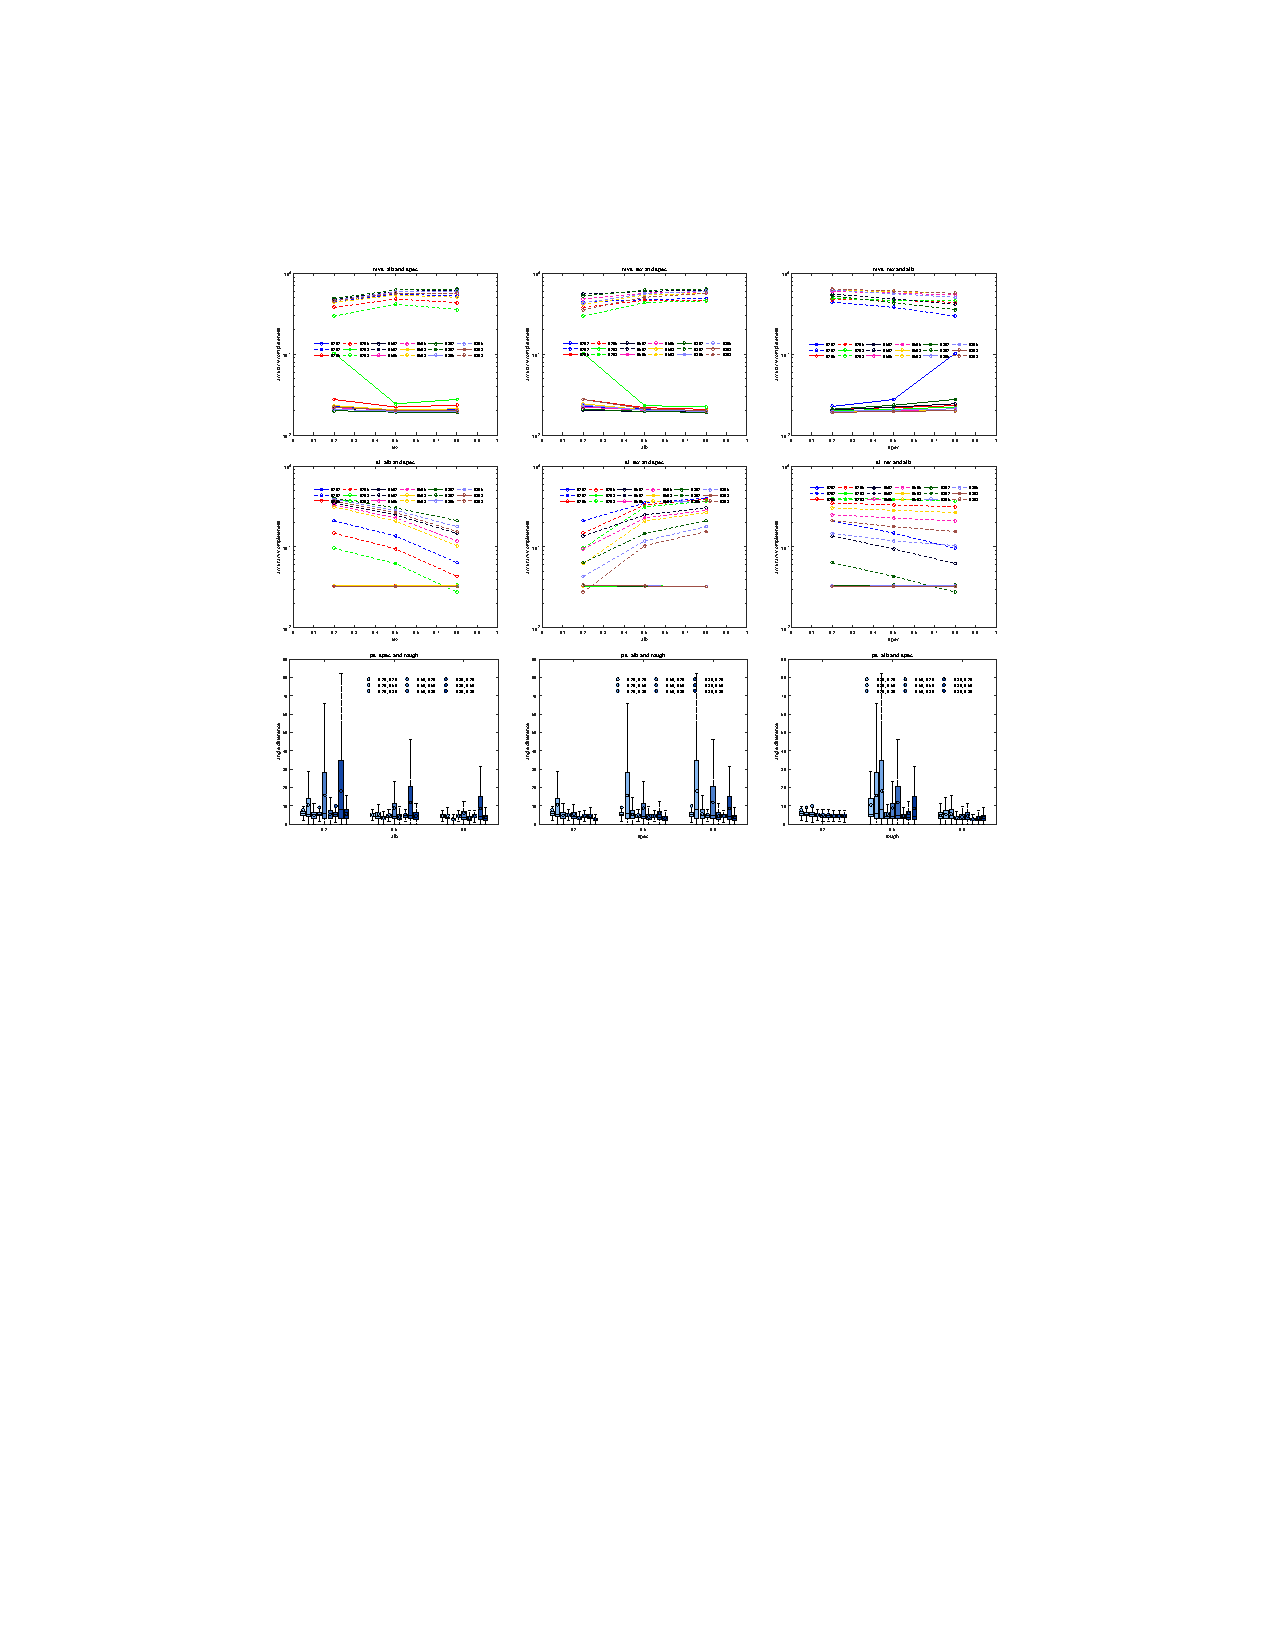
\includegraphics[width=\textwidth]{training/training}
\caption{Performance of MVS, SL and PS with varied properties. Each each column, we fix one property while changing the others, thus the second and the third columns are essentially the same as the first column, they are just different point of views of looking at those relations. Each line/boxplot represents a different combinations of property values: 0202, 0205, 0208, 0502, ..., 0808. Beware that we consider \{tex, alb, spec\} for MVS and SL, and \{alb, spec, rough\} for SL.}
\label{fig:training}
\end{figure}

\section{Summary}


%% The following is a directive for TeXShop to indicate the main file
%%!TEX root = diss.tex

\chapter{Interpretation of 3D Reconstruction Model}
\label{ch:3DRecon_Interp}

From the analysis of how algorithms perform on images which contain similar properties, a single algorithm can be definitively chosen based on which performed best on the training images.

Three techniques from different categories have been implemented. They are: PMVS, example-based PS, gray-code SL.
%\include{discussion}
%\include{conclusions}

%    3. Notes
%    4. Footnotes

%    5. Bibliography
\begin{singlespace}
\raggedright
\bibliographystyle{abbrvnat}
\bibliography{biblio}
\end{singlespace}

\appendix
%    6. Appendices (including copies of all required UBC Research
%       Ethics Board's Certificates of Approval)
%\include{reb-coa}	% pdfpages is useful here
%% The following is a directive for TeXShop to indicate the main file
%%!TEX root = diss.tex
\chapter{Supporting Materials}

% This would be any supporting material not central to the dissertation.
% For example:
% \begin{itemize}
% \item radiometry
% \item technical details of MVS, PS, SL, SfS, etc
% \end{itemize}

\section{Definition of 3D Reconstruction}
\label{sec:3DRecon_Def}
We will first provide definitions of some basic concepts, which include general computer vision concepts such as scene, camera, and image. We then define a few other terms that are closely related to the reconstruction problem. We then provide reasonable approximations for a more practical definition of the problem as a whole.

\subsection{Basic notations}
We will use the following notations: $\{C_n\}_{n=0}^{N-1}$ represents the camera set, which includes both intrinsic and extrinsic parameters; $\{I_n\}_{n=0}^{N-1}$ represents the set of all images; $\{L_n\}_{n=0}^{N-1}$ represents the set of light sources.

\noindent\textbf{Definition 1 (Scene)} The scene $S$ is the four-dimensional joint spatio-temporal target of interest.

\noindent\textbf{Definition 2 (Image)} The image refers to the 2D observation of the 3D scene $S$ on the image plane of camera $C_i$ at time $t_0$, which is modelled as: $I_i = T(S, C_i, L_0, t_0)$, or on the image plane of $C_0$  under the light source $L_i$ at time $t_i$, $I_i= T(S, C_0, L_i, t_i)$, where $T$ is the geometric/radiometric transformation.

$T$ can be a geometric transformation which determines the 2D coordinates of a 3D point, or a radiometric transformation which determines the intensity/irradiance information from the information of illumination, viewing direction and surface orientation.

\subsection{Segment and Scell}
\noindent\textbf{Definition 3 (Segment)} A segment ($seg$) is a distinct region in the image, and is the most basic element in the image, which can be considered as a generalized pixel. 

For instance, a segment can be a pixel, a window area, an edge, a contour, or a region of arbitrary size and shape.

\noindent\textbf{Definition 4 (Cue)} Cues are the visual or geometric characteristics of the segments $seg$ that can be used for reconstruction, denoted as $cue(seg)$.

For instance, the cue can be the texture within a window area, the intensity/colour value of a pixel, or the object contour, etc.

\noindent\textbf{Definition 5 (Scell)} A scell (scene element, denoted as $sc$) is a volume in the scene which corresponds to at least one segment. A scell can be considered as a generalization of a voxel.
 % However, a scell is not necessarily distinct since

\noindent\textbf{Definition 6 (Property)} Properties are the visual and geometric characteristics of the scell $sc$, which would influence the cues of a segment, denoted as $prop(sc)$.

The property of the scell can be the 3D position or orientation information, visual texture, reflectance, surface orientation, roughness, convacity, etc.

The relation between the terms defined above is shown in Figure~\ref{fig:scell_seg}.
\begin{figure}[!htbp]
\centering
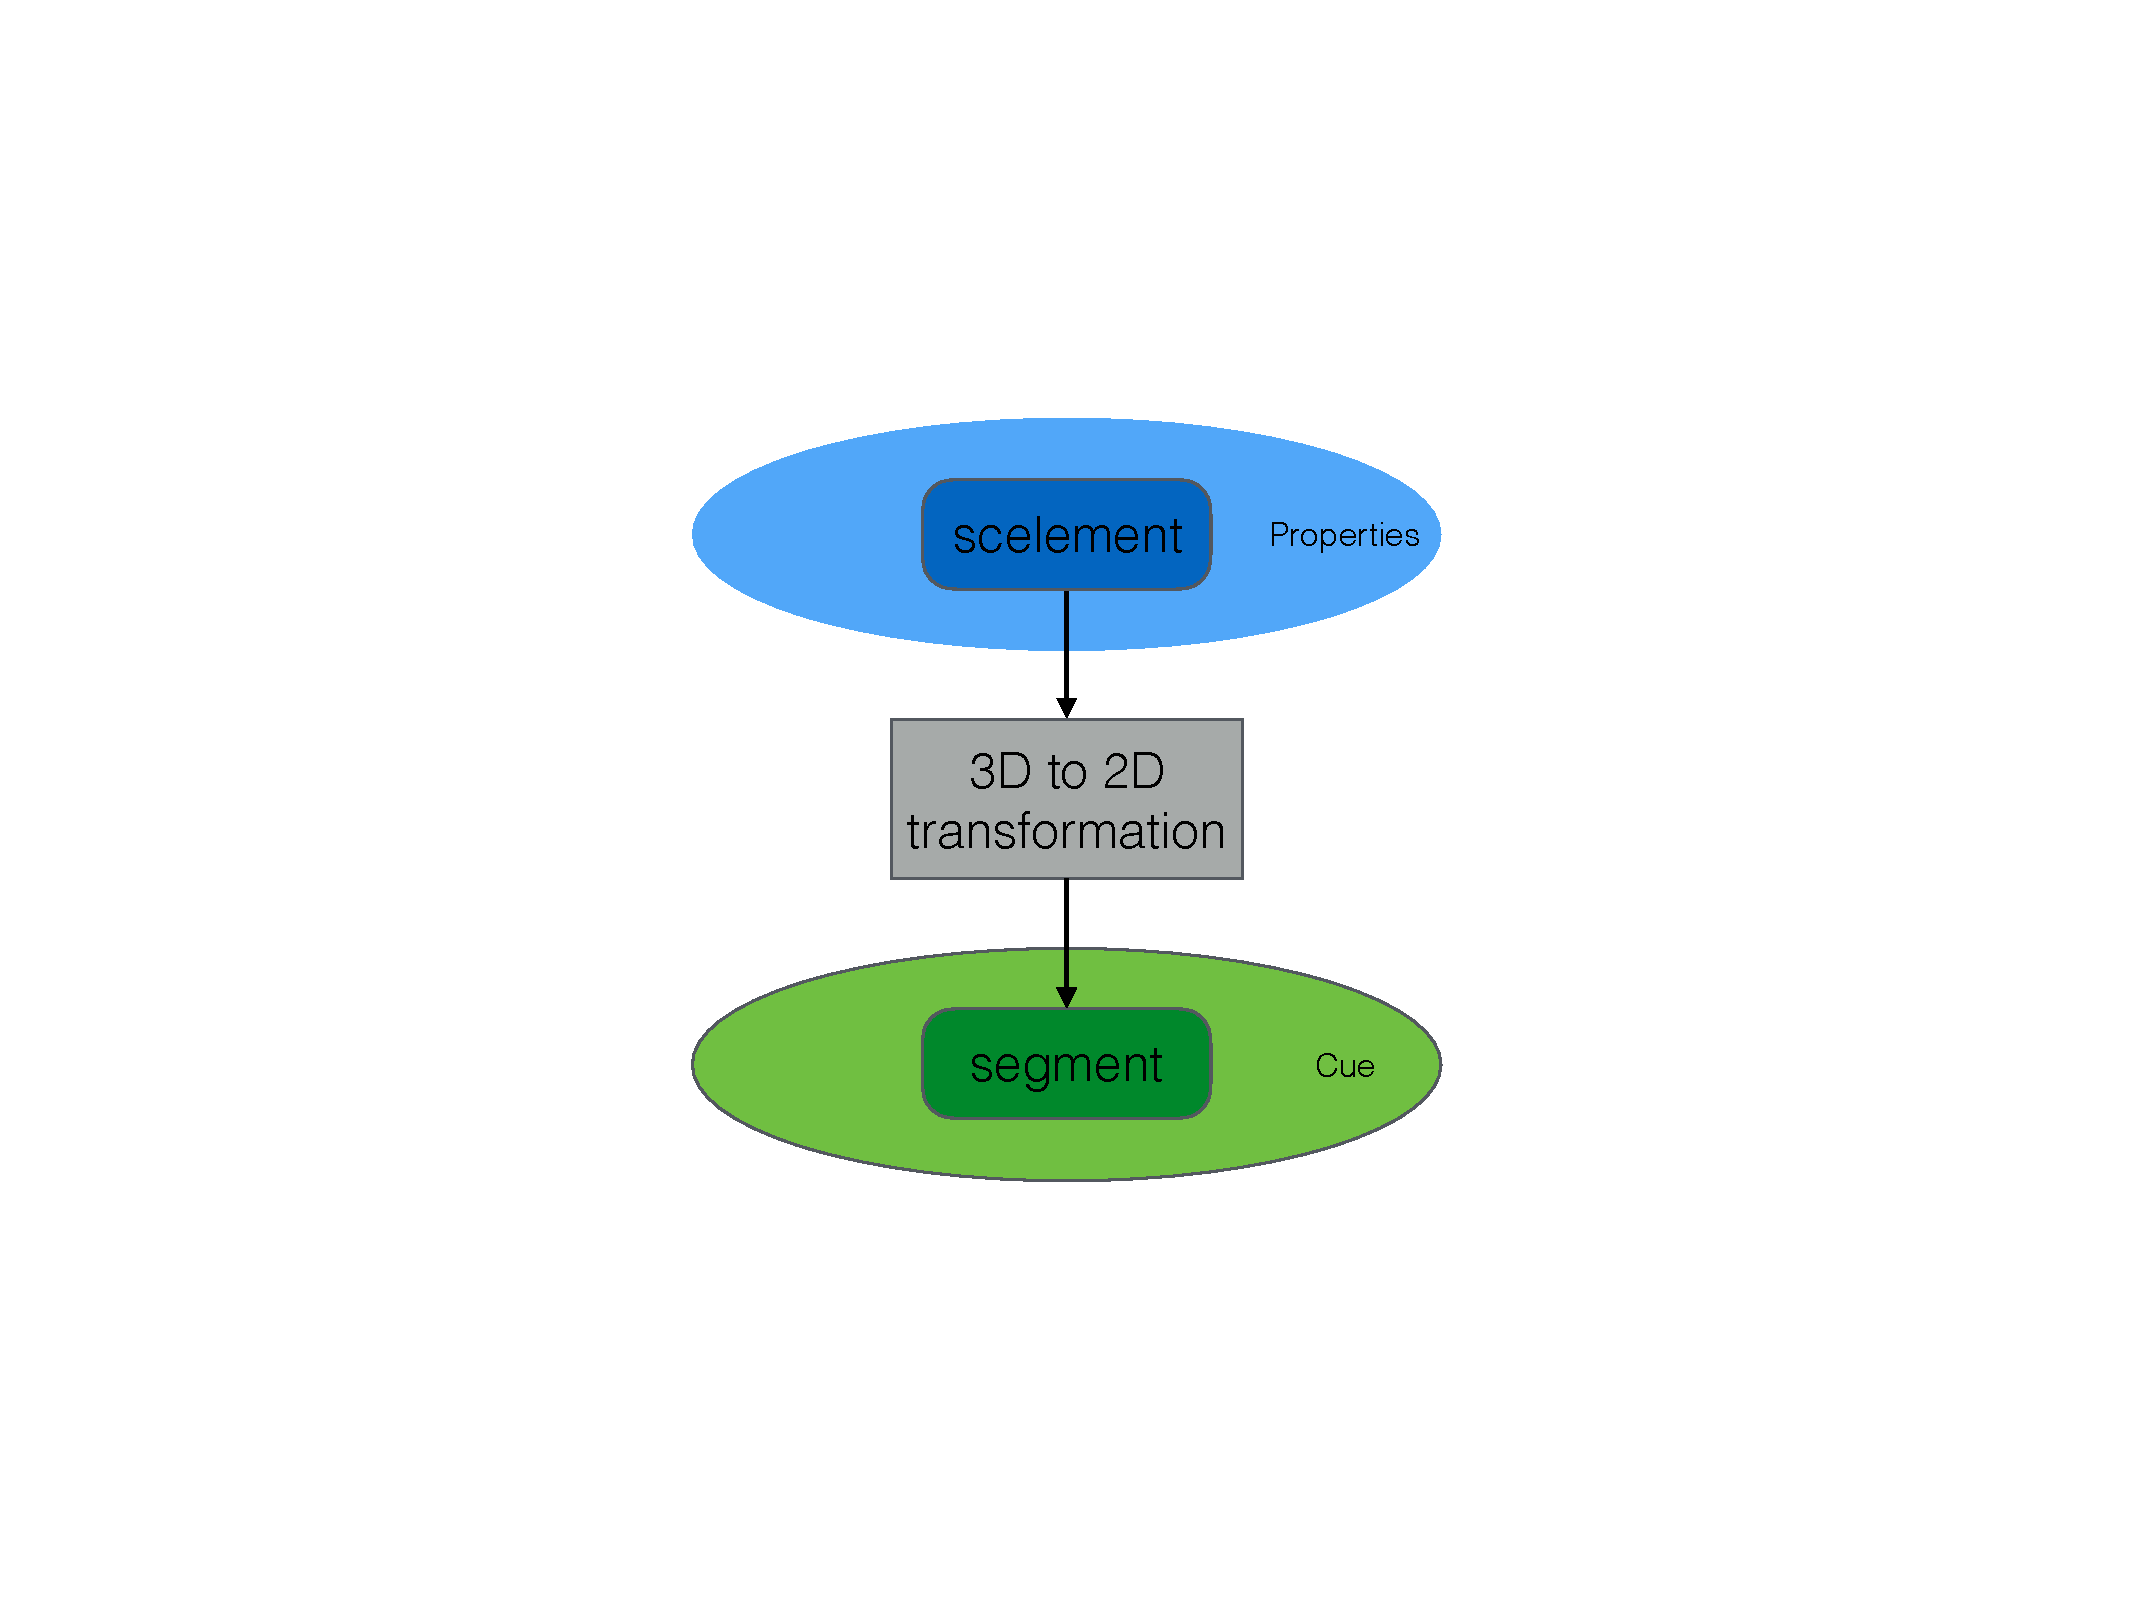
\includegraphics[width=0.5\textwidth]{model/seg_scell}
\caption{Relation between a scell and a segment}
\label{fig:scell_seg}
\end{figure}

% \textbf{Definition (Representation)} The scell can be represented as a voxel, a depth value, a 3D point/patch, or a surface normal, etc, which is denoted as $rep(sc)$.

\subsection{Consistency}
Every photograph of a 3D scene taken from a camera $C_i$ partitions the set of all possible scenes into two families, those that reproduce the photograph and those that do not. We characterize this constraint for a given shape and a given radiance assignment by the notion of \textit{consistency}.

\noindent\textbf{Definition 7 (Consistency criterion)} The consistency criterion checks whether the properties of a scell $sc$ can produce the cues observed in the corresponding segment $seg$.
\begin{align*}
consist(prop(sc), cue(seg)) = 1 &\Rightarrow \textit{consistent}\\
consist(prop(sc), cue(seg)) = 0 &\Rightarrow \textit{not consistent}
\end{align*}

\noindent\textbf{Definition 8 (Segment consistency)} Let $S$ be the scene. A scell $s\in S$ that is visible from $C_i$ is consistent with the image $I_i$ if and only if the consistency criterion is true.

\noindent\textbf{Definition 9 (Image consistency)} A scene $S$ is image consistent with image $I_i$ if any scell $\forall s\in S$ visible from the camera $C_i$ is segment consistent with this image.

\noindent\textbf{Definition 10 (Scene consistency)} A scene $S$ is scene consistent with a set of images $\{I_n\}_{n=0}^{N-1}$ if it's image consistency with each image $I_i\in \{I_n\}_{n=0}^{N-1}$ in the set.

\subsection{Formal Definition}
\noindent\textbf{Definition 11 (3D reconstruction problem)} Given a set of images $\{I_n\}_{n=0}^{N-1}$ captured by cameras $\{C_n\}_{n=0}^{N-1}$, or under a set of light sources $\{L_n\}_{n=0}^{N-1}$, find a set of scells $\{sc_m\}_{m=0}^{M-1}$ such that any scell is consistent with the visible images in the set $\{I_n\}_{n=0}^{N-1}$, \ie $\forall sc_i\in \{sc_m\}_{m=0}^{M-1}$, we the have following:
\begin{align*}
consist(prop(sc_i), cue(seg_{(i, j)})) = 1.
\end{align*}
where $seg_{(i, j)}$ is the corresponding segment of $sc_i$ in camera $C_j$. Alternatively, 3D reconstruction tries to find a set of scells $\{sc_m\}_{m=0}^{M-1}$ that are scene consistent with the image set $\{I_n\}_{n=0}^{N-1}$

\subsection{Applied Definition}
While the definition presented above gives a formal definition of the problem of 3D reconstruction, it is not necessarily applicable in a practical setting. In this section, we extend this formal definition to an approximate, yet applied version.

\noindent\textbf{Definition 12 (Consistency score)} The consistency score measures the similarity betweem a scell $sc$ and the corresponding segment $seg$.
\begin{align*}
consist(prop(sc), cue(seg)) &= x \text{, } x\in[0, 1]\\
consist(prop(sc), cue(seg)) &= 1 \Rightarrow \textit{consistent}\\
consist(prop(sc), cue(seg)) &= 0 \Rightarrow \textit{not consistent}
\end{align*}

\noindent\textbf{Definition 13 (Applied consistency criterion)} A scell $sc$ and a segment $seg$ are considered consistent if the the consistency score is above a pre-defined threshold $\epsilon$.
$$
consist(prop(sc), cue(seg)) > \epsilon
$$

% \noindent\textbf{Some more definitions} $\sum_{n\in I'}consist(prop(sc_i), cue(seg_{(i, n)}))$

\noindent\textbf{Definition 14 (Applied 3D Reconstruction Problem)} Given a set of images $\{I_n\}_{n=0}^{N-1}$ captured by cameras $\{C_n\}_{n=0}^{N-1}$, or under a set of light sources $\{L_n\}_{n=0}^{N-1}$, find a set of scells $\{sc_m\}_{m=0}^{M-1}$ such that the consistency score between the set of scells and their corresponding segments $\{seg_{(i, j)}\}_{i=0,j=0}^{M-1,N-1}$ are maximized.
$$
\mbox{maximize} \quad \sum_{j=0}^{N-1}\sum_{i=0}^{M-1} consist(prop(sc_i), cue(seg_{(i, j)}))
$$

\section{Definition of Radiometric Terms}
\label{sec:radio_term}
Below is a list of radiometry terms, see Figure~\ref{fig:radiometry_terms} for an illustration:
\begin{itemize}
\item Solid angle ($d\omega$): 3D counterpart of angle, $d\omega=\frac{dA \cos\theta_i}{R^2}\mathit{ (steradian)}$.
\item Projected solid angle ($d\Omega$): $d\Omega = \cos\theta d\omega$.
\item Incident radiance ($\mathbf{L_i(\theta_i, \phi_i)}$): light flux received from the direction $(\theta_i, \phi_i)$ on a unit surface area, unit $\mathit{ (watt\cdot m^{-2}\cdot steradian^{-1})}$.
\item Irradiance ($\mathbf{E_i(\theta_i, \phi_i)}$): light Flux (power) incident per unit surface area from all direction, $\mathbf{E_i(\theta_i, \phi_i)}=\int_{\Omega_i} L_i(\theta_i, \phi_i) d\Omega_i \mathit{ (watt/m^2)}$.
\item Surface radiance ($\mathbf{L_r(\theta_r, \phi_r)}$): light flux emmited from a unit surface area in the direction $(\theta_r, \phi_r)$, unit $\mathit{ (watt\cdot m^{-2}\cdot steradian^{-1})}$.
\end{itemize}

\begin{figure}[!htbp]
\centering
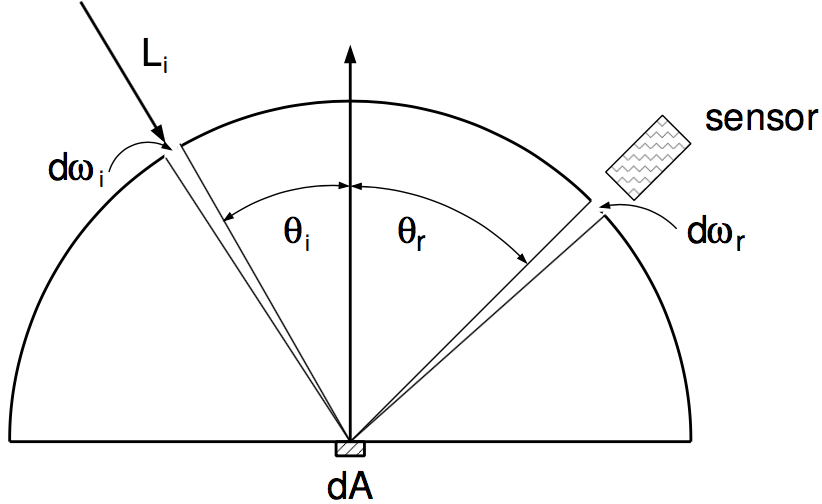
\includegraphics[width=0.5\textwidth]{model/radiometry_terms.png}
\caption{Illustration of light-matter interaction.}
\label{fig:radiometry_terms}
\end{figure}

\section{Material of real-world objects}
\label{sec:real_world_dataset}
\begin{table}[!hbtp]
  \centering
  \begin{tabular}{*{9}{c}}
  \multicolumn{3}{l}{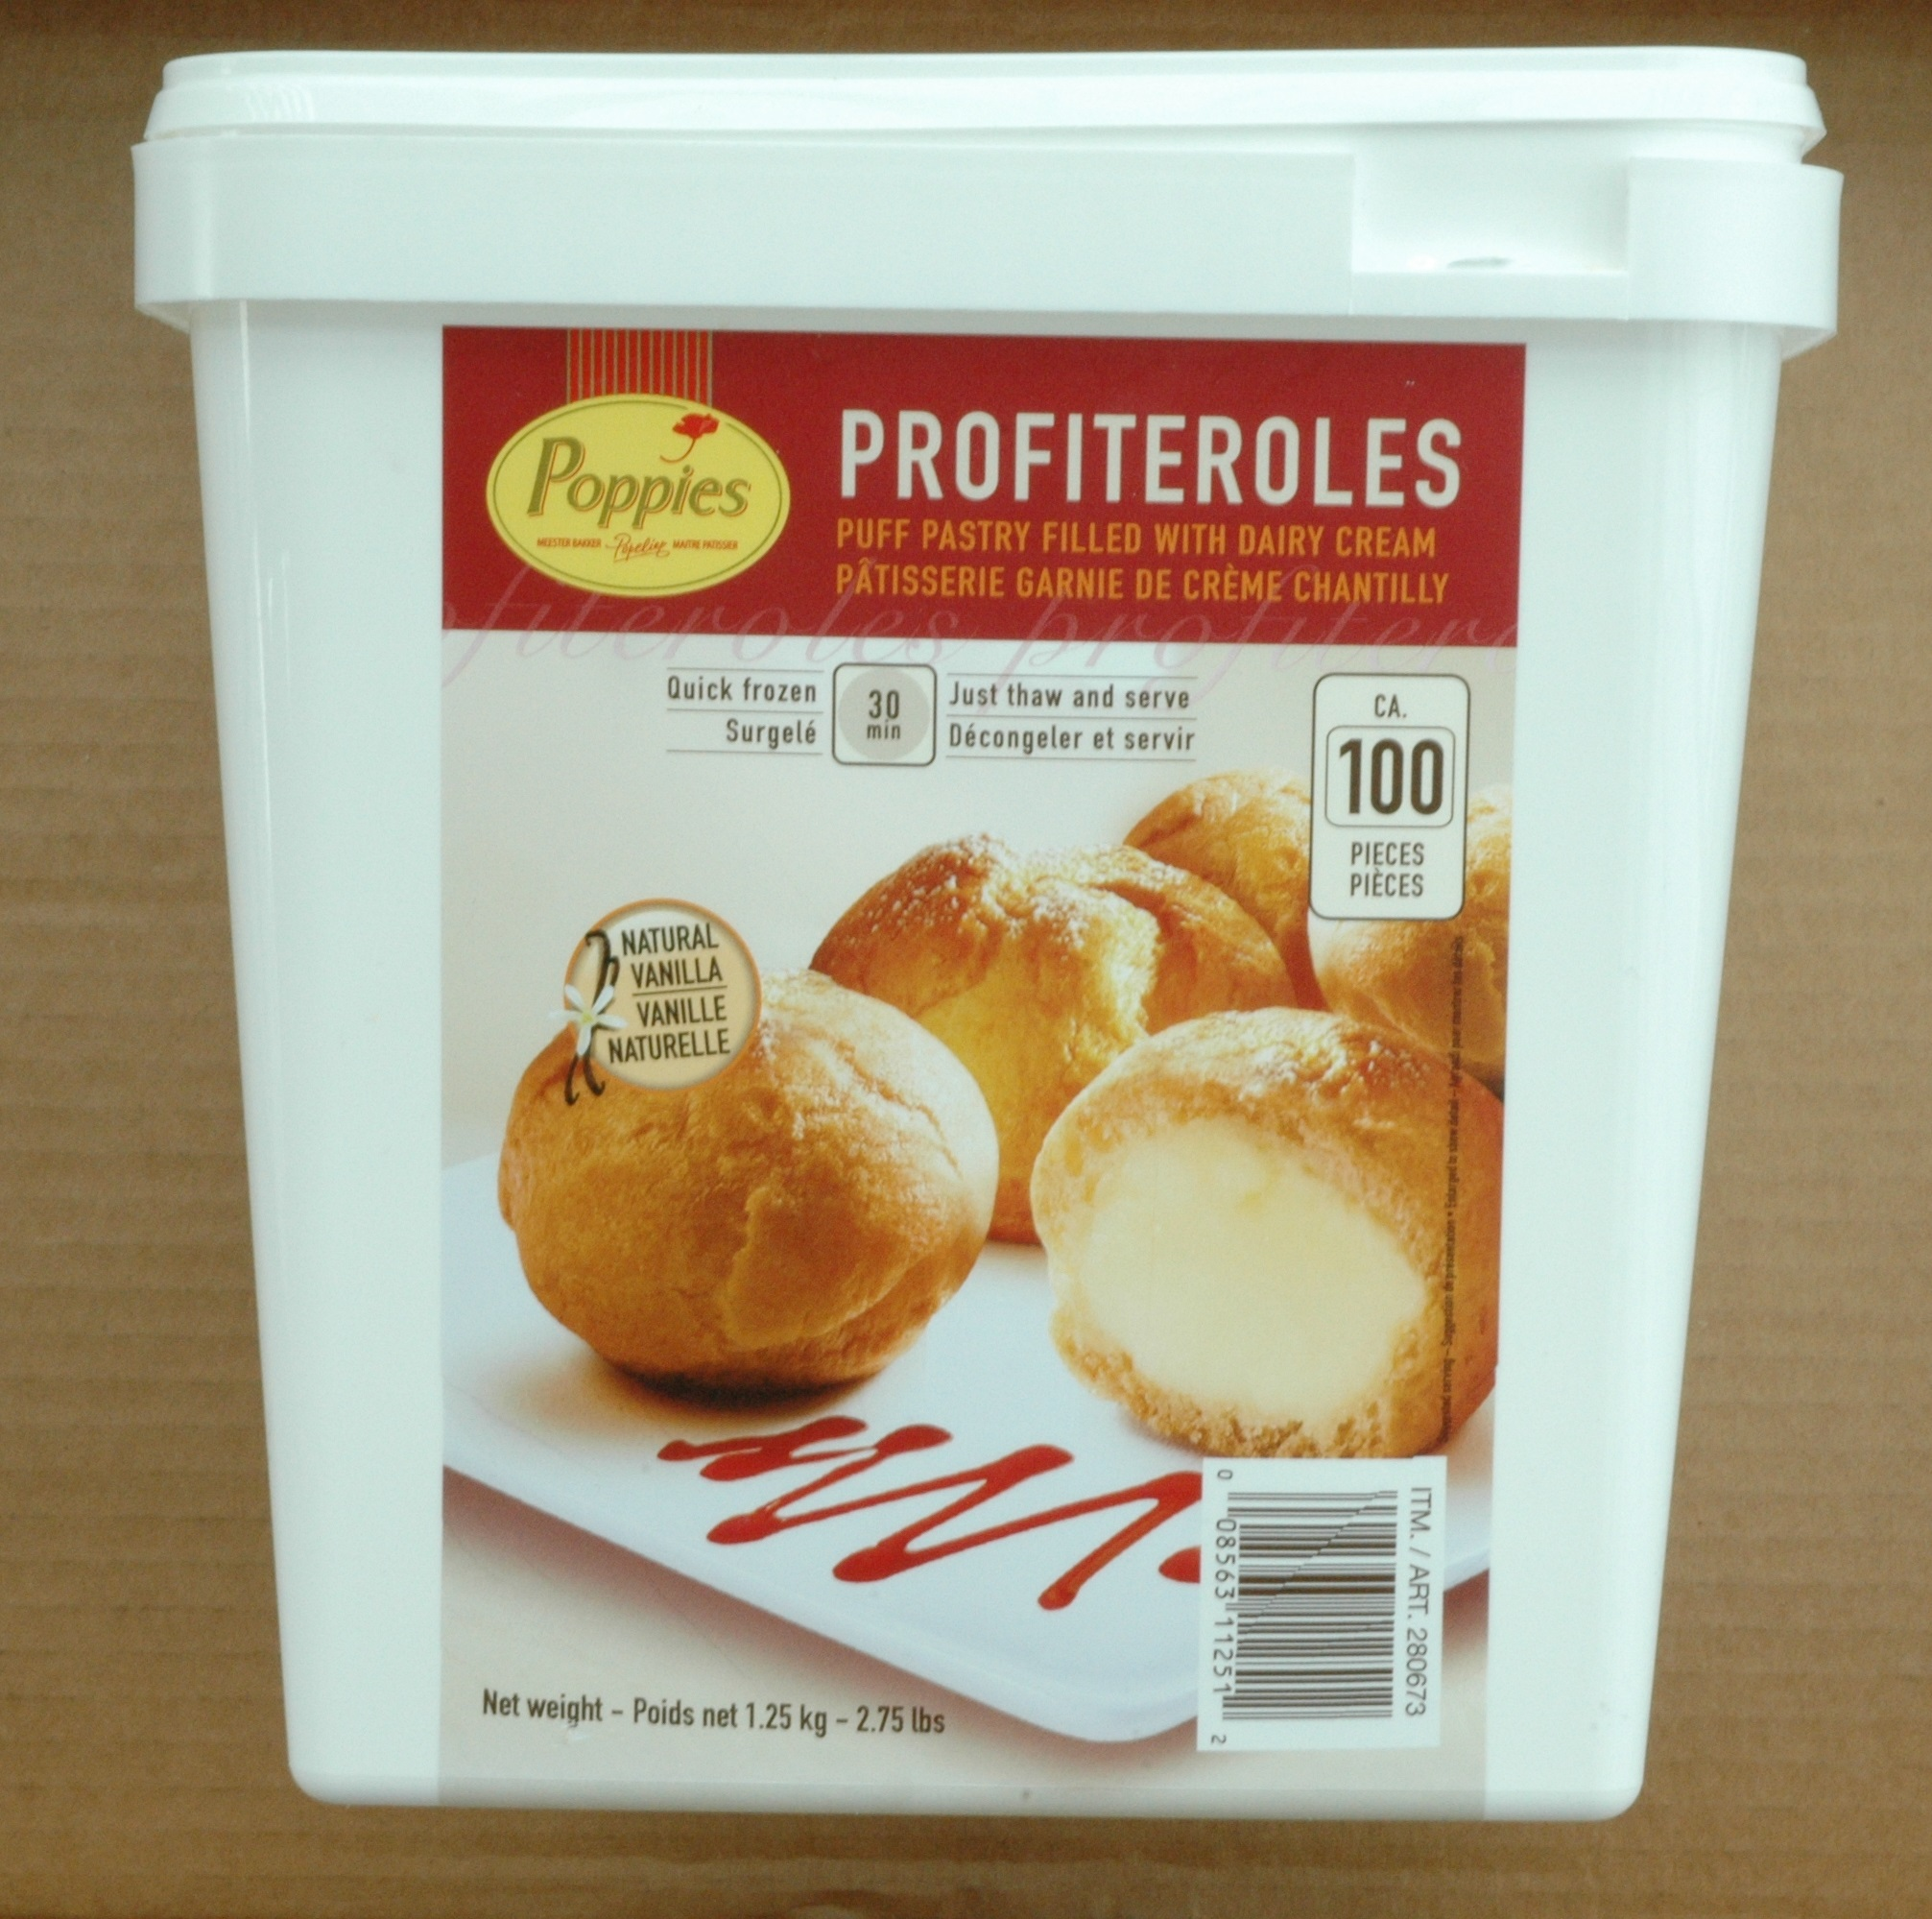
\includegraphics[width=0.33\textwidth]{interp/real_world_img/box/box}} &
  \multicolumn{3}{l}{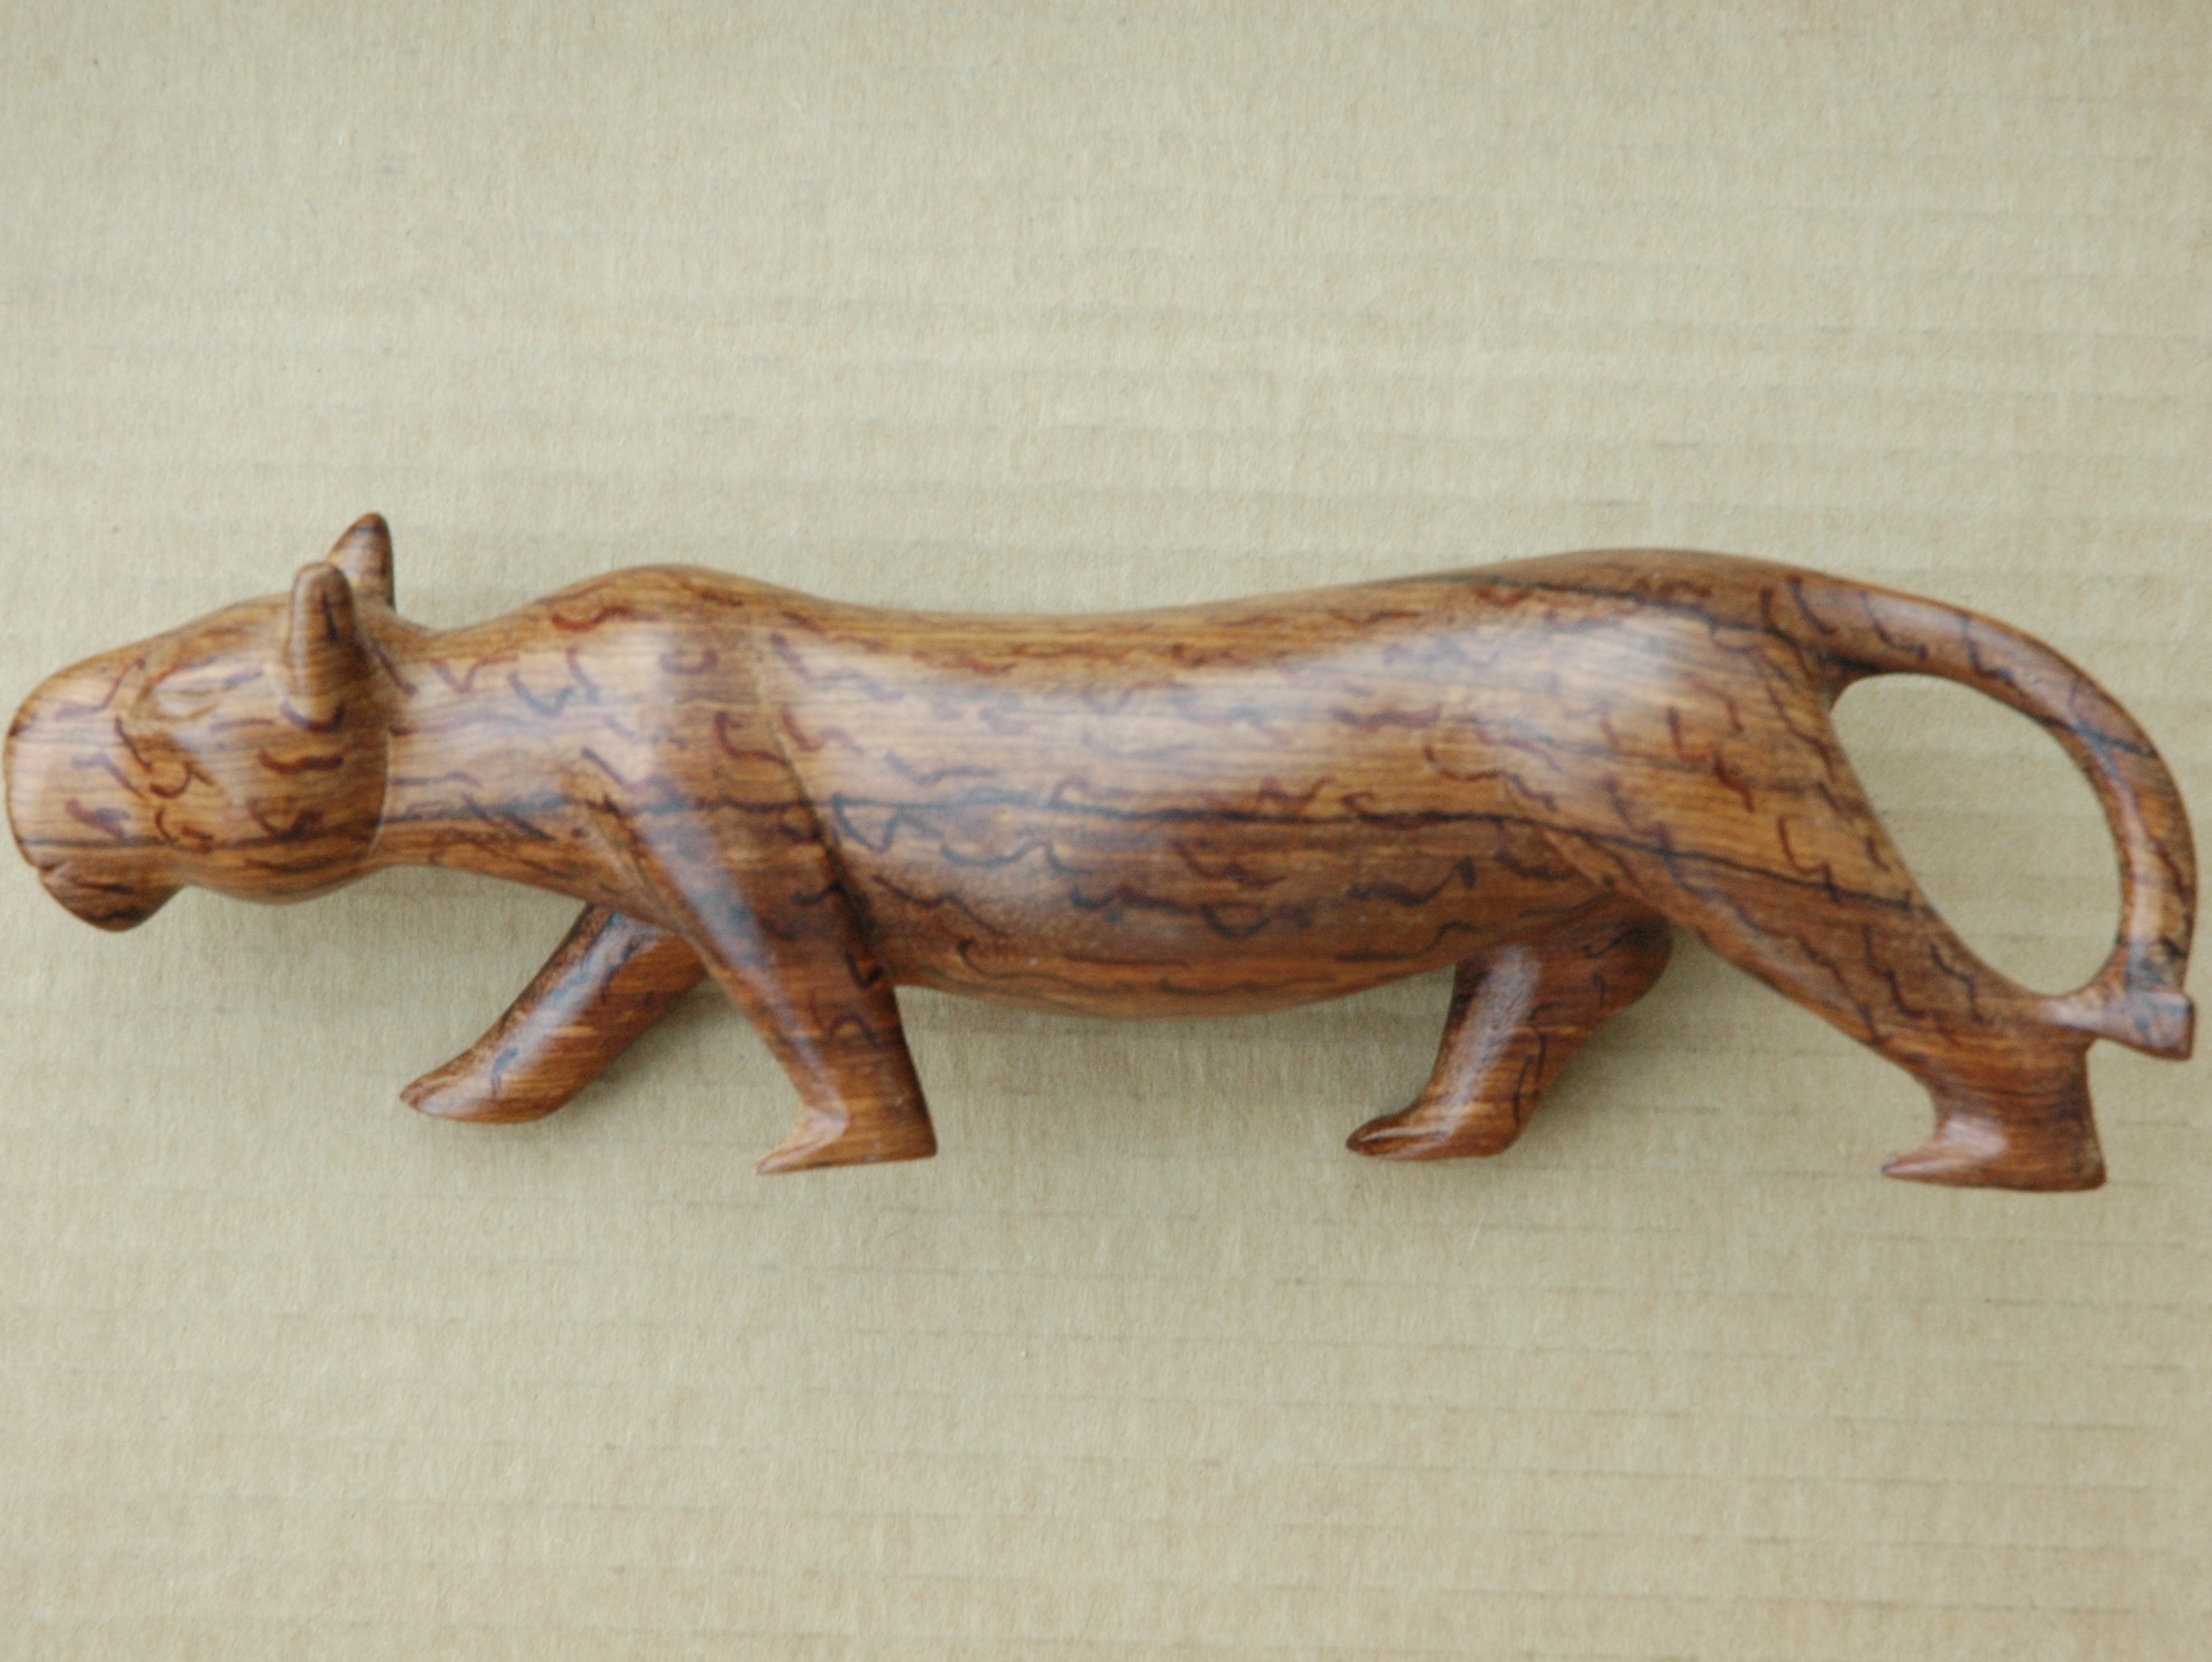
\includegraphics[width=0.33\textwidth]{interp/real_world_img/cat0/cat0}} &
  \multicolumn{3}{l}{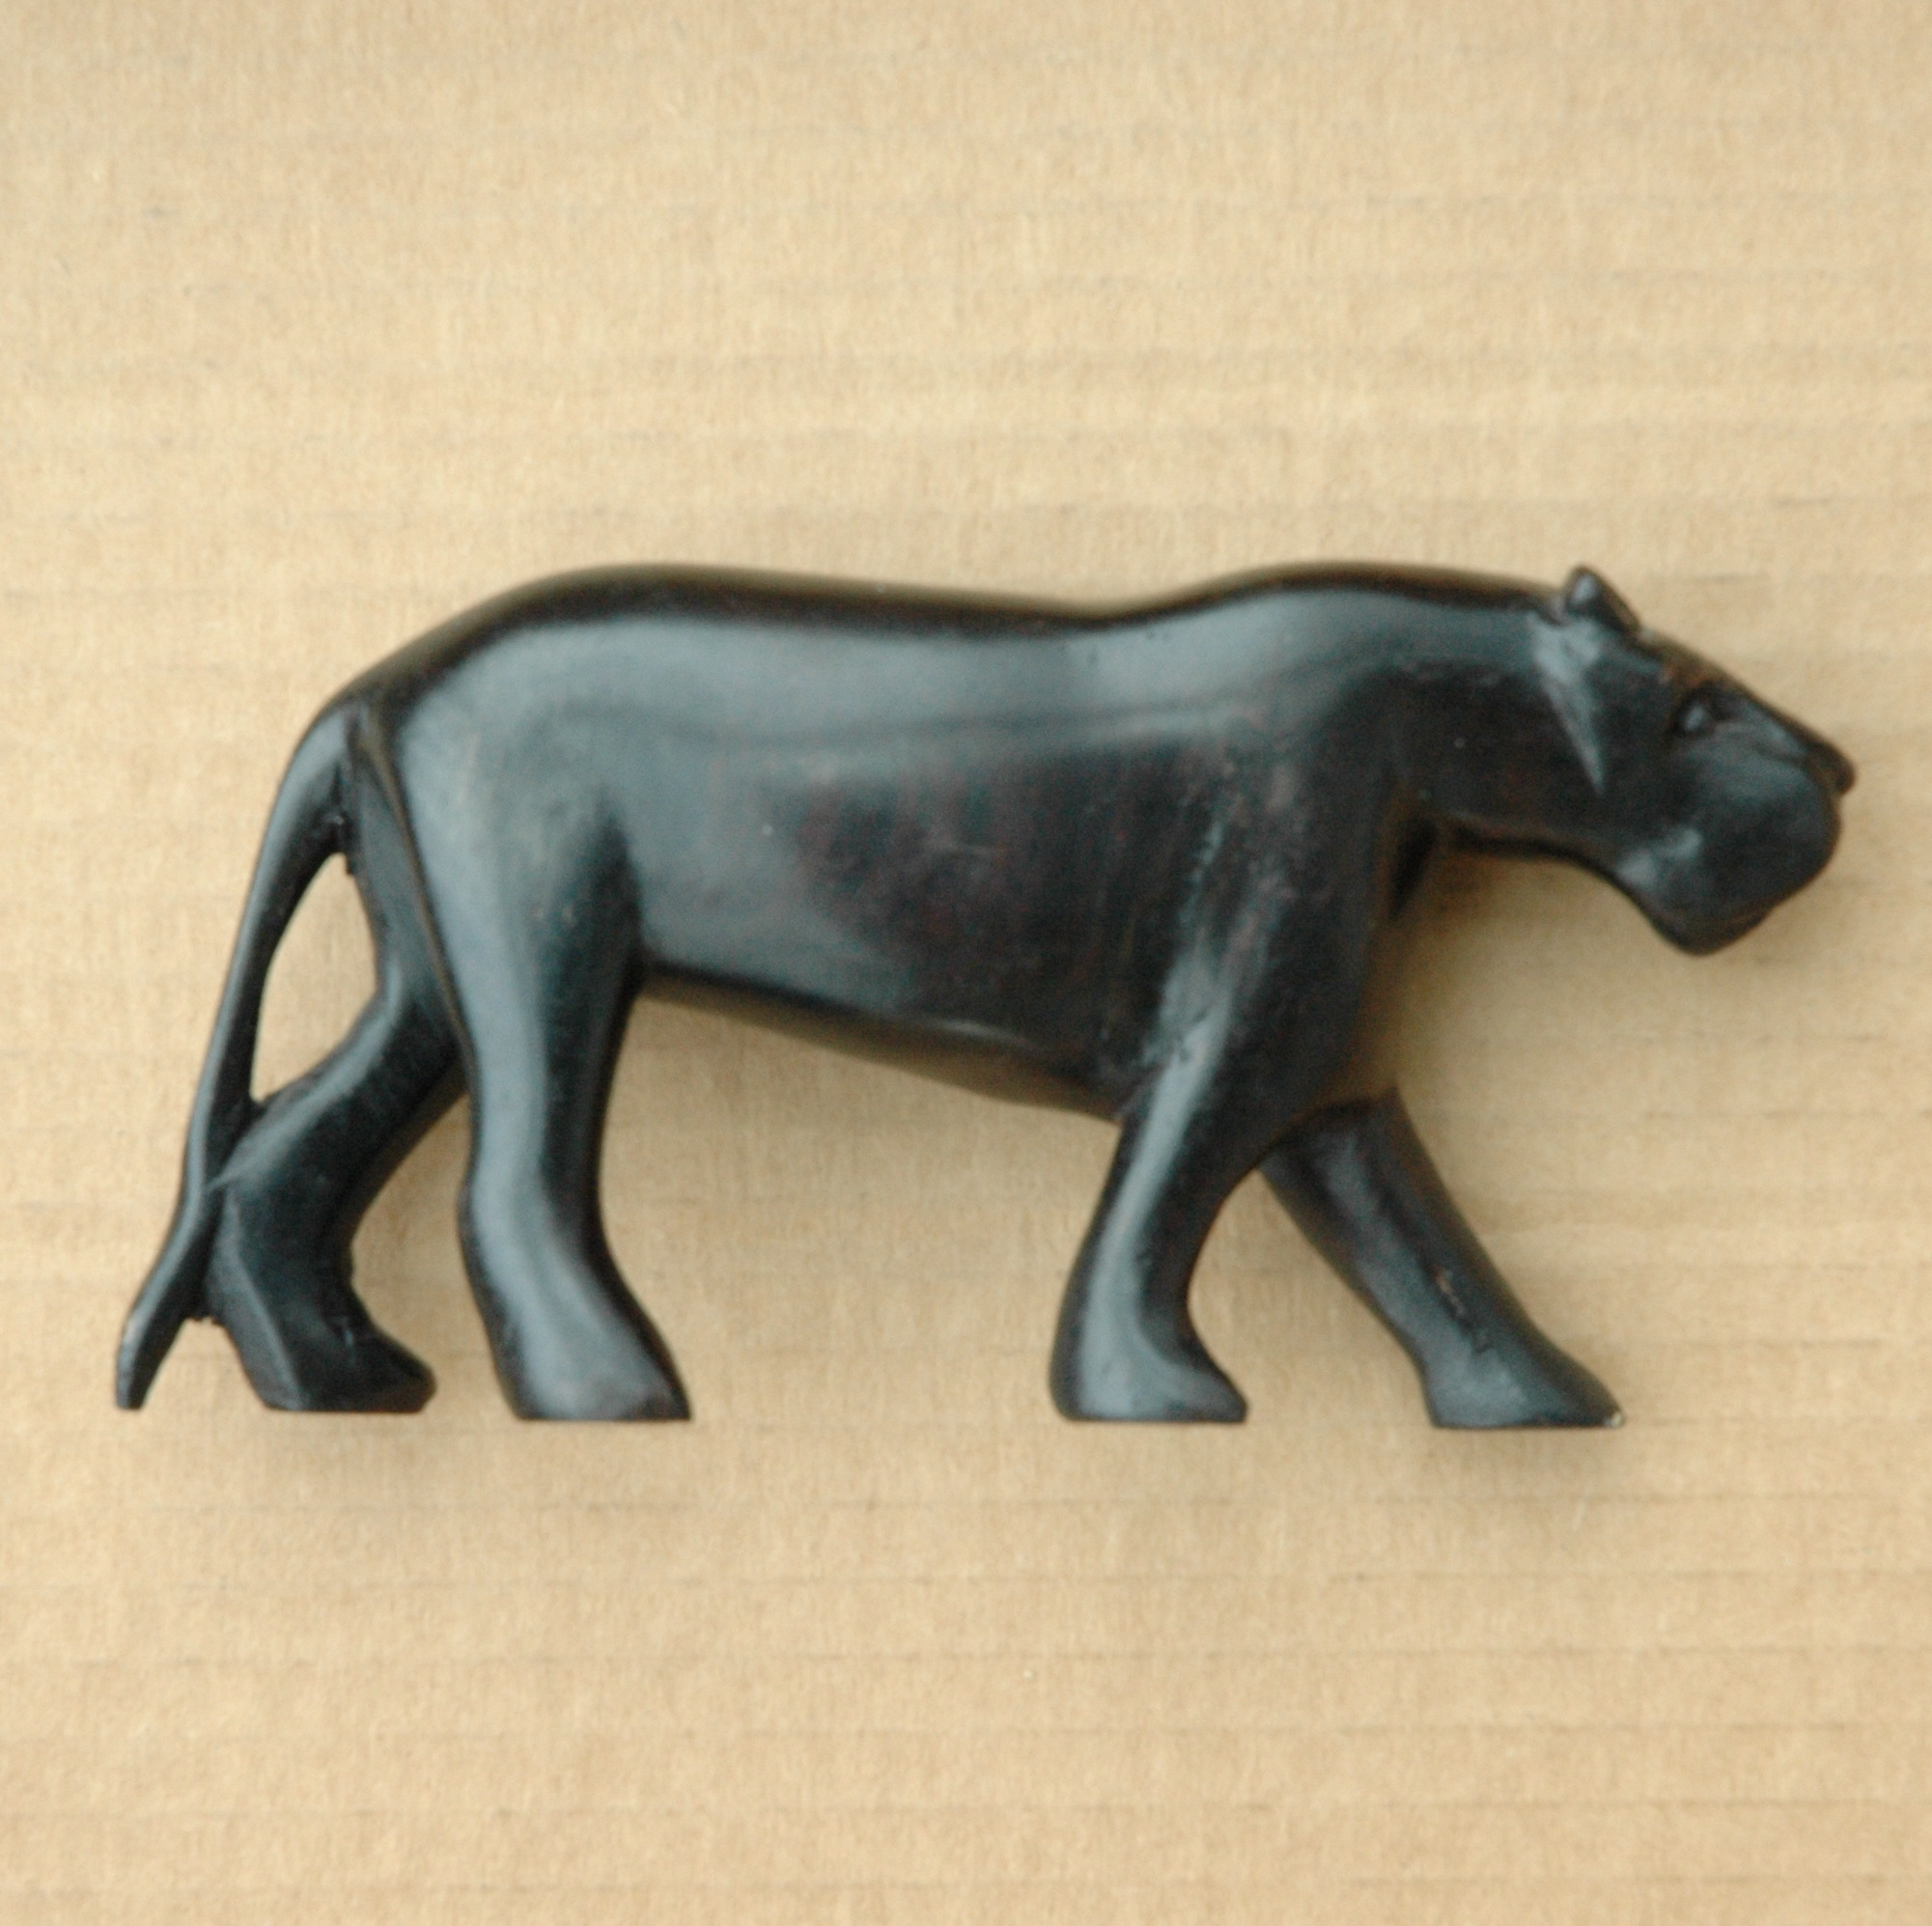
\includegraphics[width=0.33\textwidth]{interp/real_world_img/cat1/cat1}}\\
  % 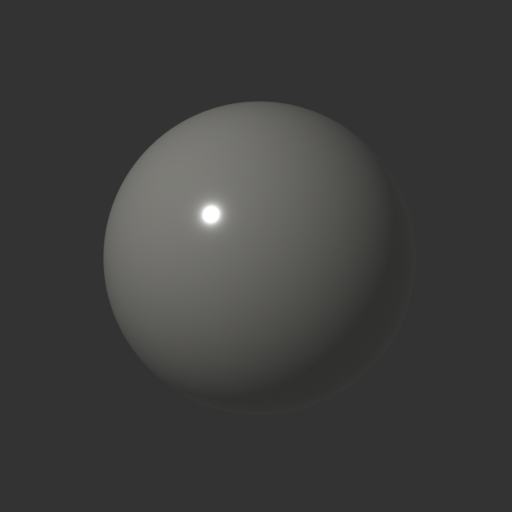
\includegraphics[width=0.1\textwidth]{interp/real_world_img/box/base_00} &
  % 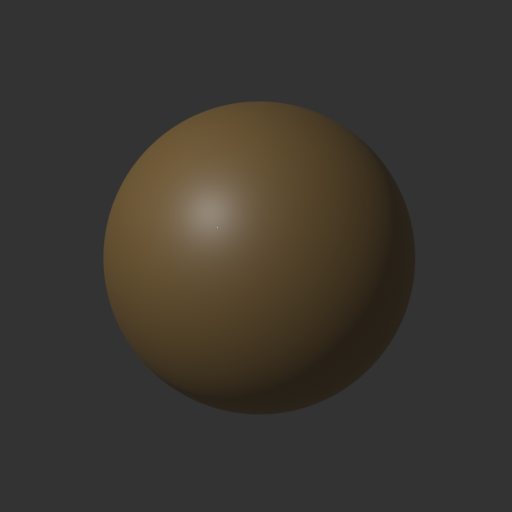
\includegraphics[width=0.1\textwidth]{interp/real_world_img/box/base_01} & 
  % 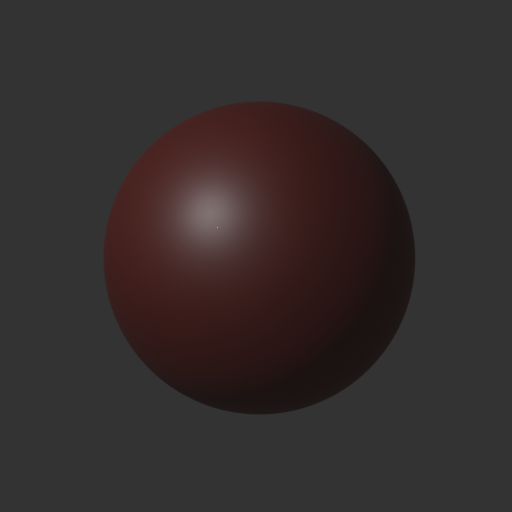
\includegraphics[width=0.1\textwidth]{interp/real_world_img/box/base_02} &
  % 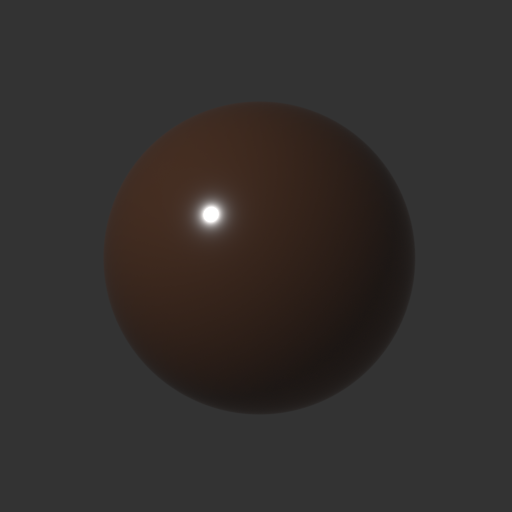
\includegraphics[width=0.1\textwidth]{interp/real_world_img/cat0/base_00} & 
  % 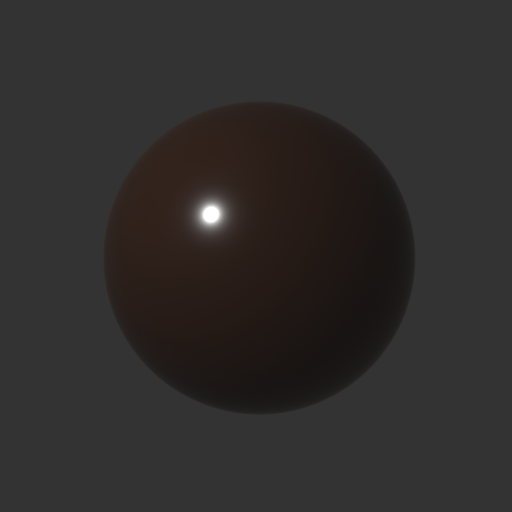
\includegraphics[width=0.1\textwidth]{interp/real_world_img/cat0/base_01}& &
  % 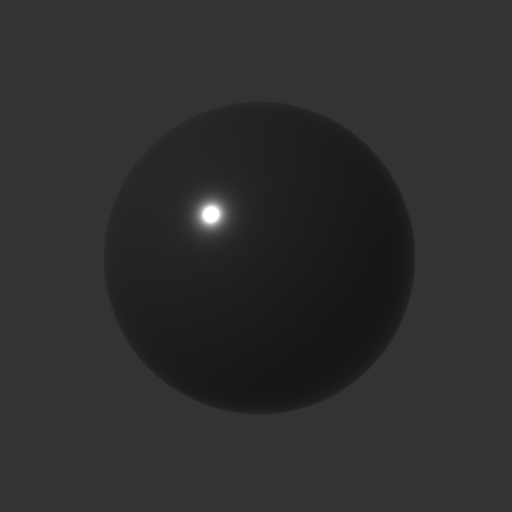
\includegraphics[width=0.1\textwidth]{interp/real_world_img/cat1/base_00} &\\
  \multicolumn{3}{c}{(a). box} & \multicolumn{3}{c}{(b). cat0} & \multicolumn{3}{c}{(c). cat1} \\
  \multicolumn{3}{l}{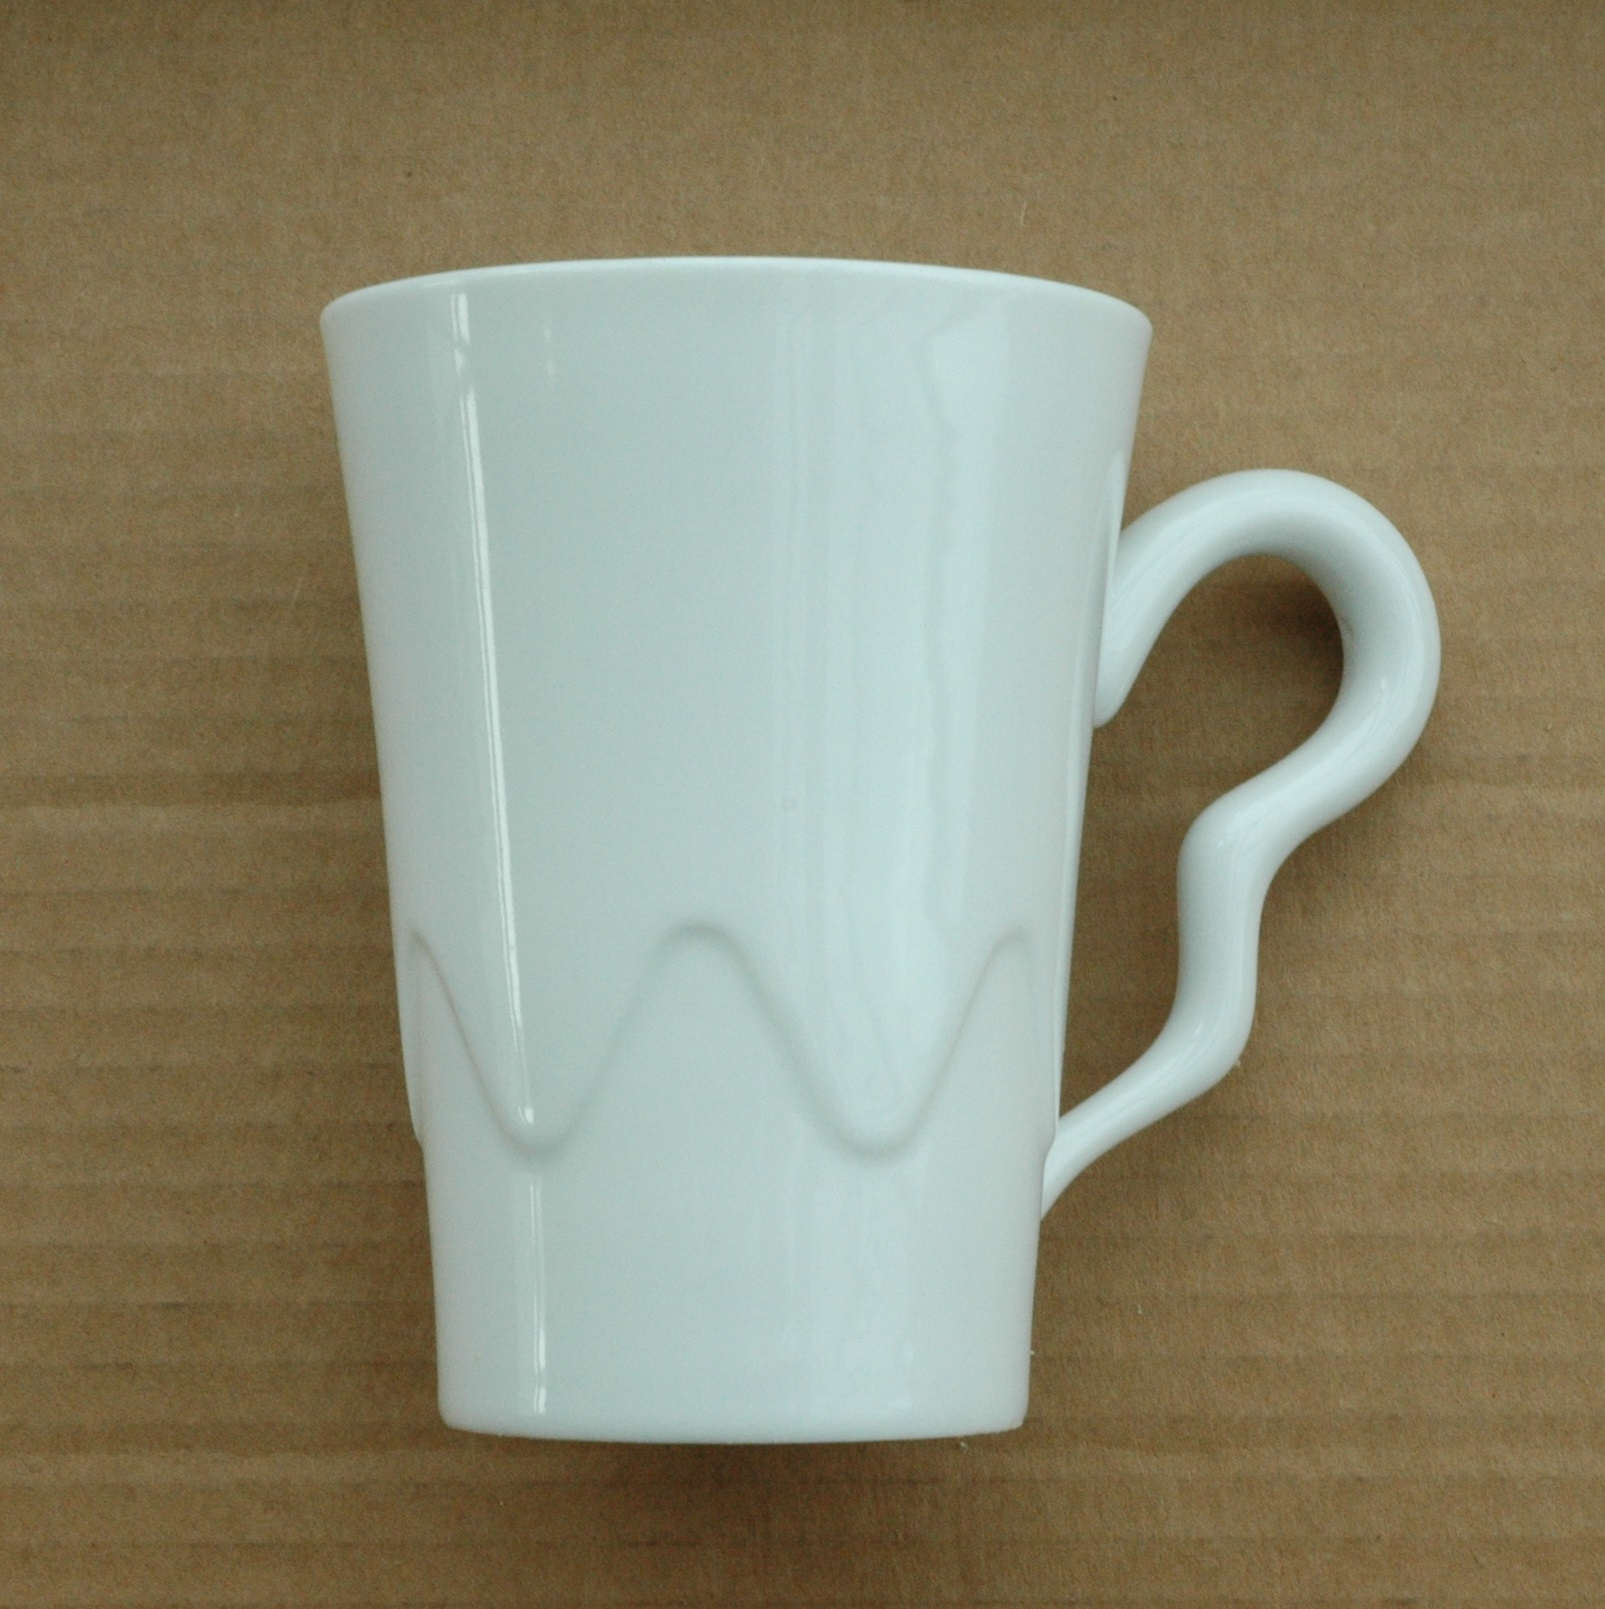
\includegraphics[width=0.33\textwidth]{interp/real_world_img/cup/cup}} &
  \multicolumn{3}{l}{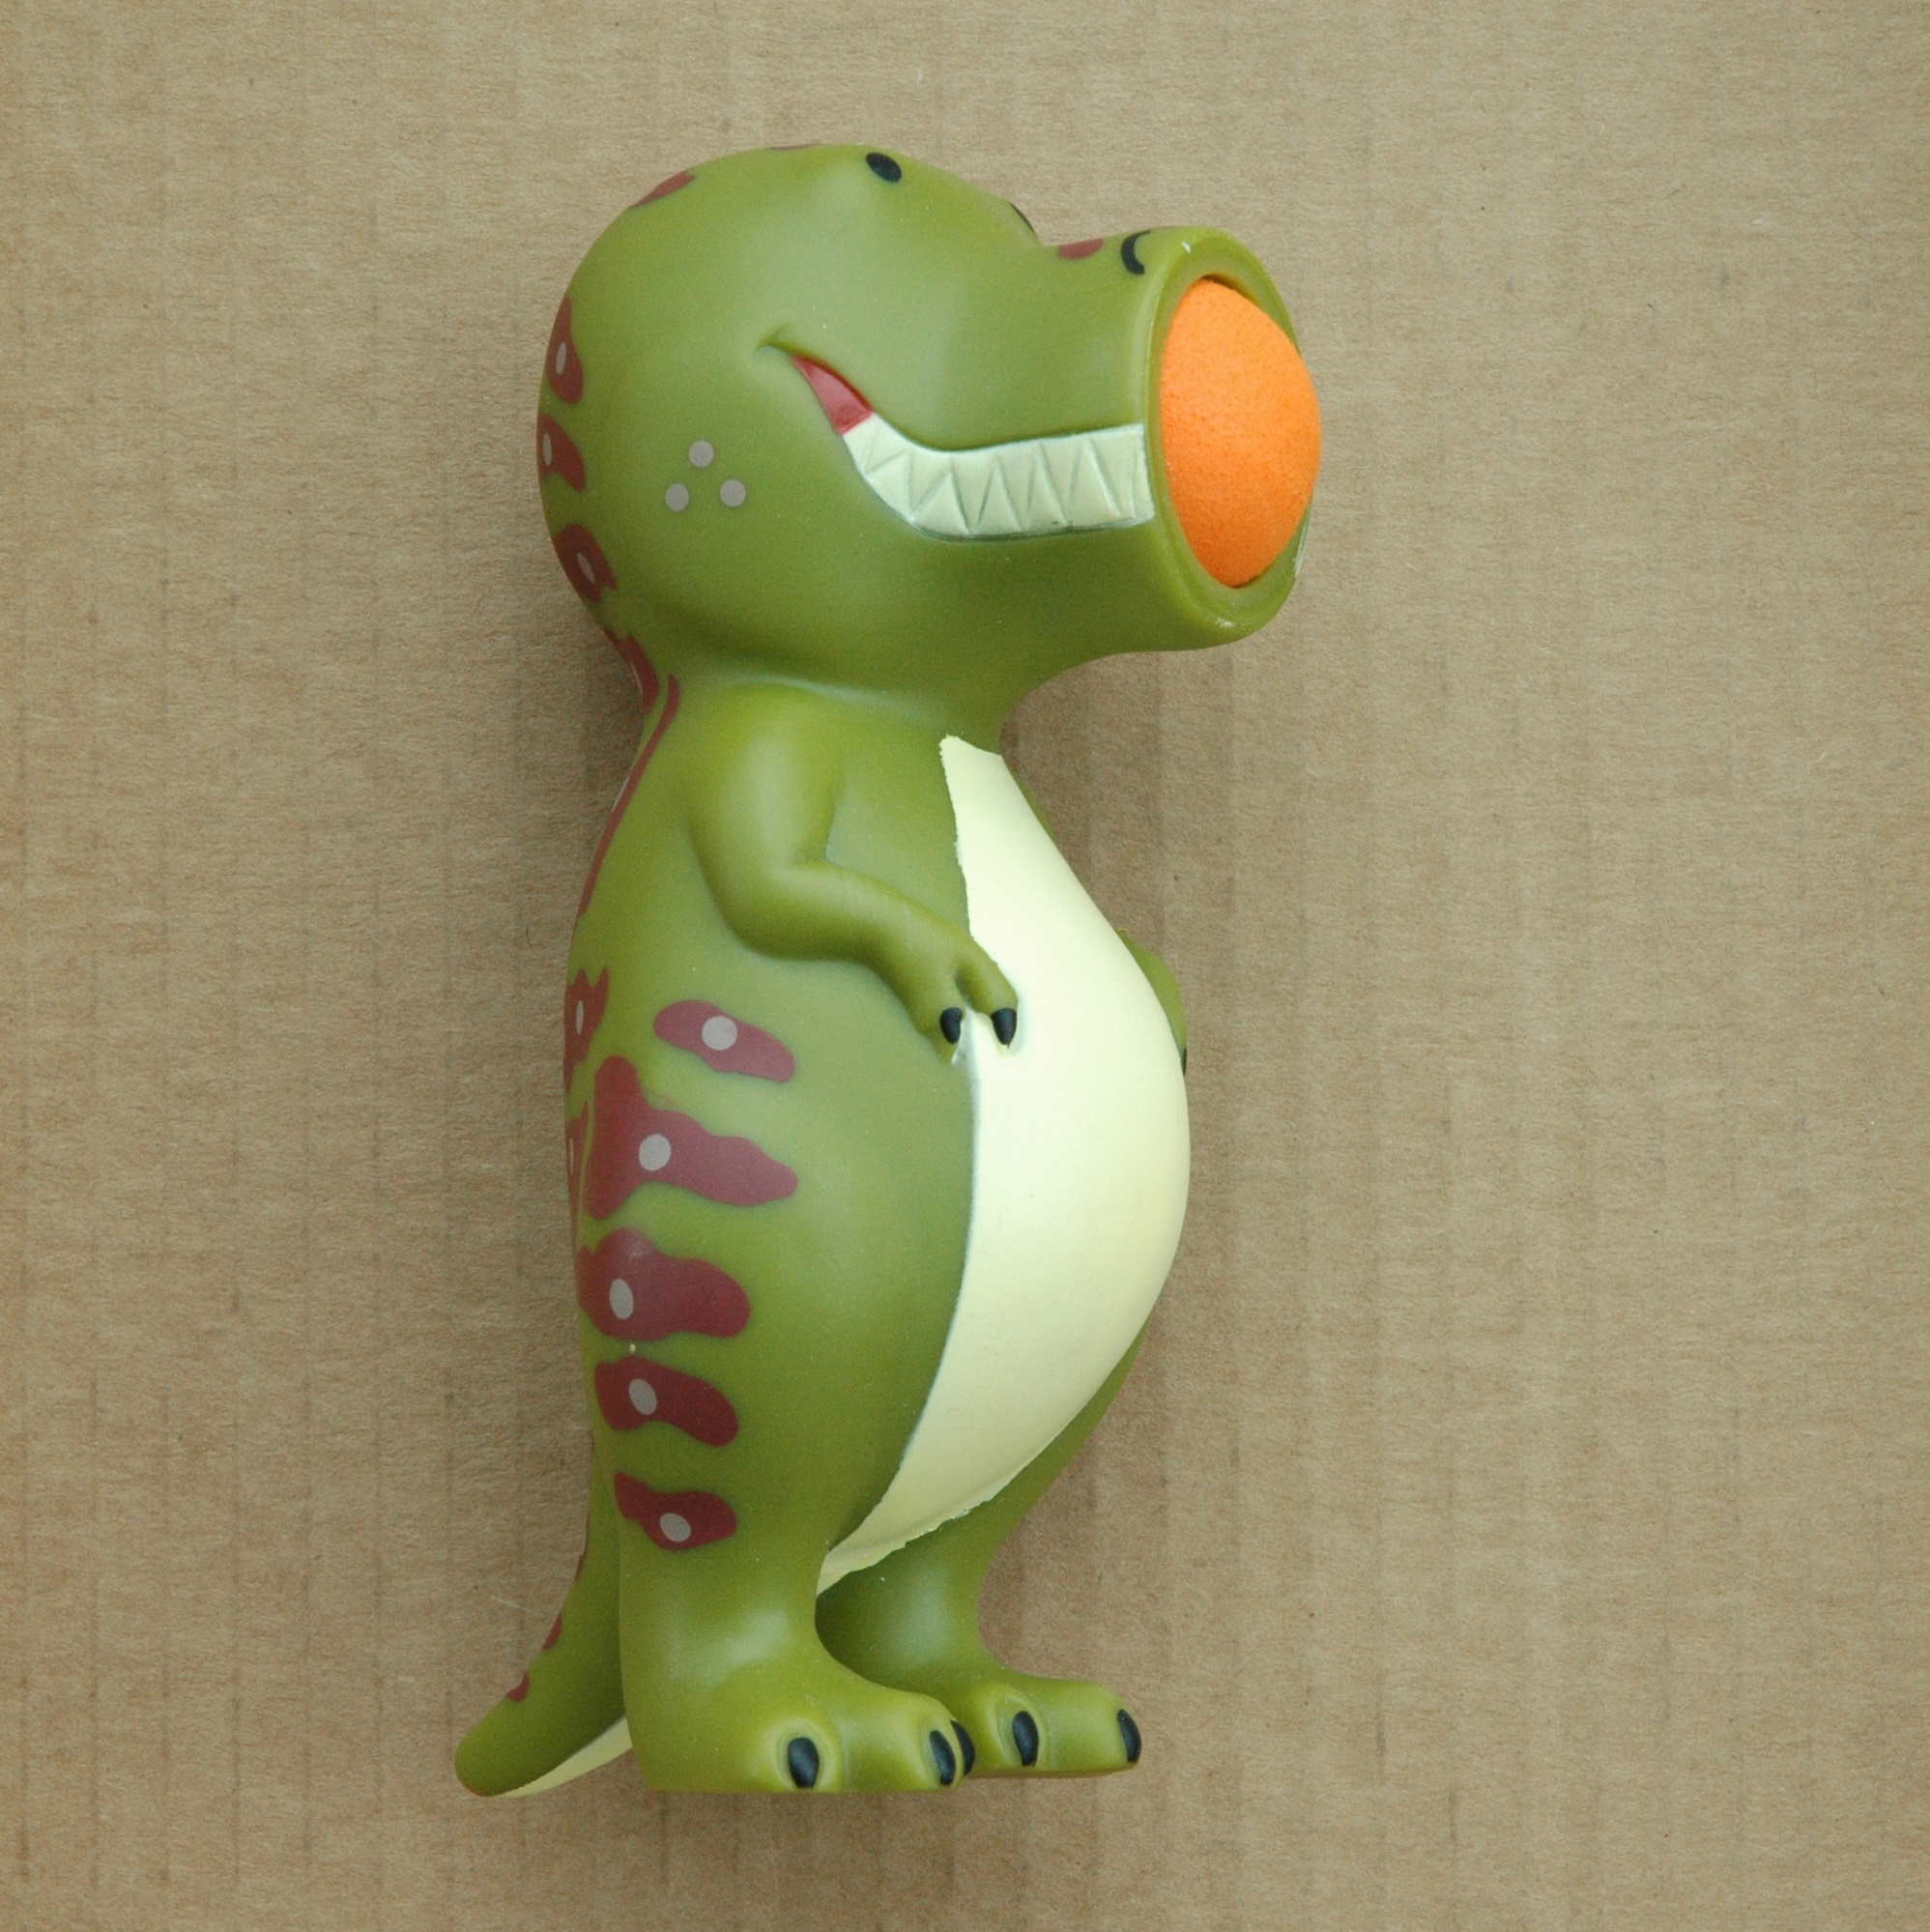
\includegraphics[width=0.33\textwidth]{interp/real_world_img/dino/dino}} &
  \multicolumn{3}{l}{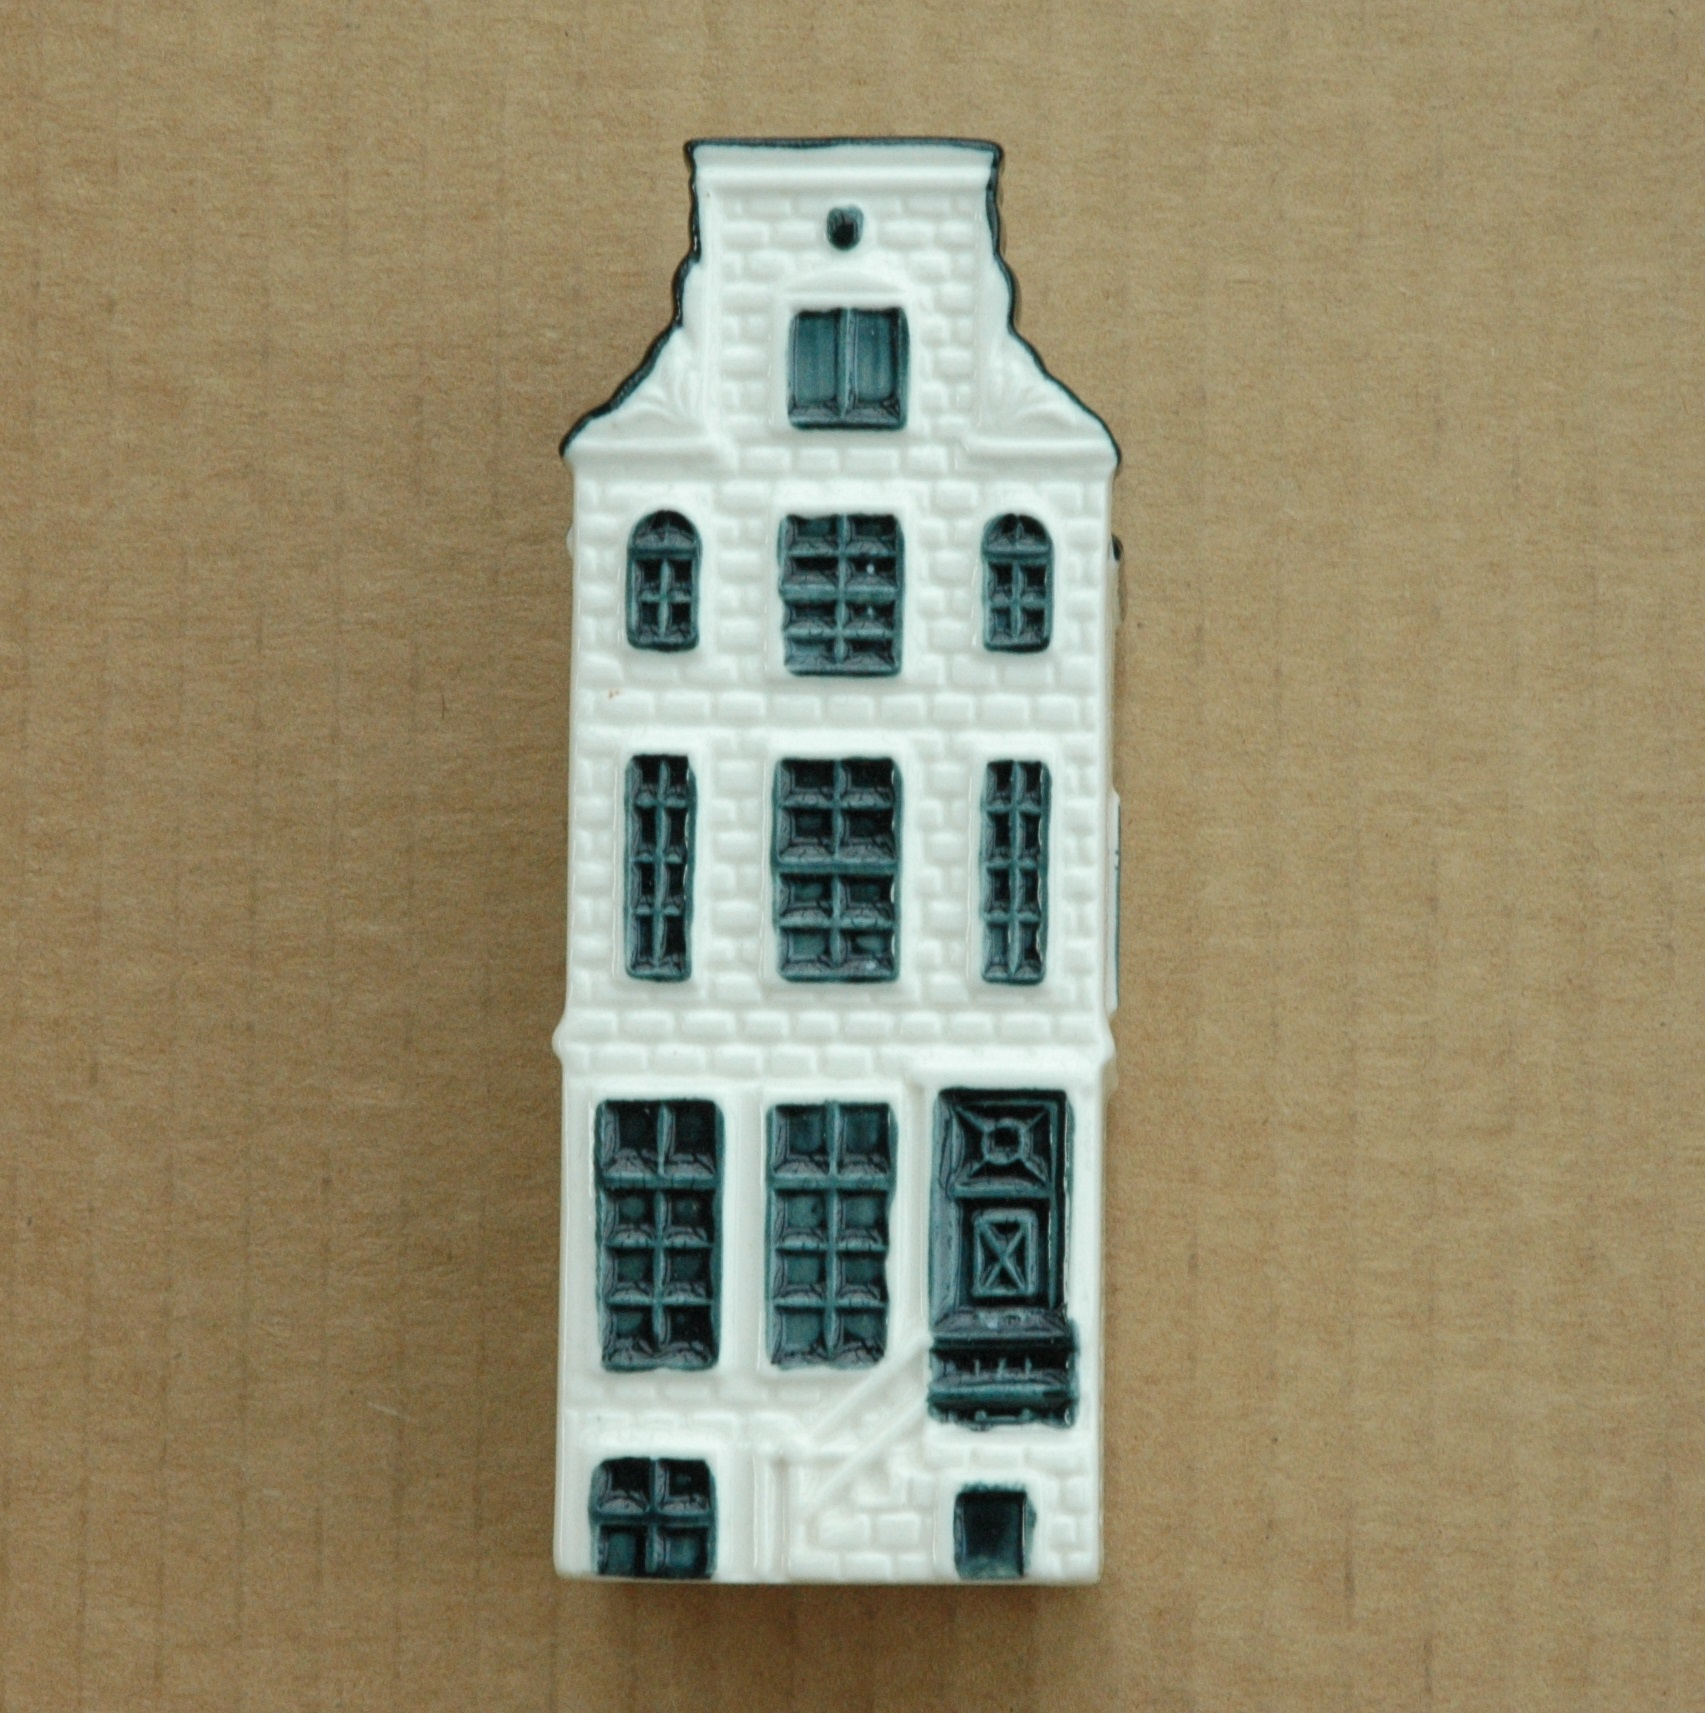
\includegraphics[width=0.33\textwidth]{interp/real_world_img/house/house}}\\
  % 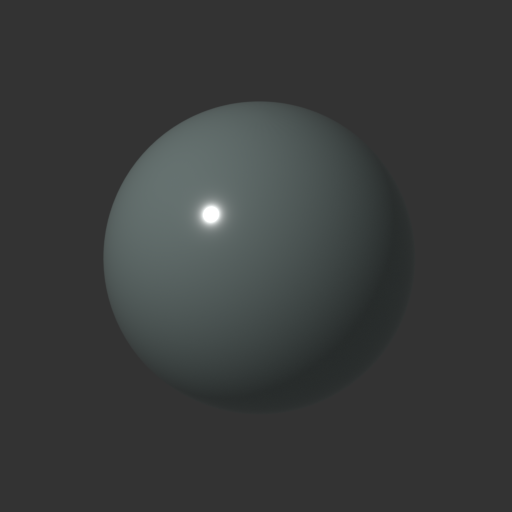
\includegraphics[width=0.1\textwidth]{interp/real_world_img/cup/base_00} & & &
  % 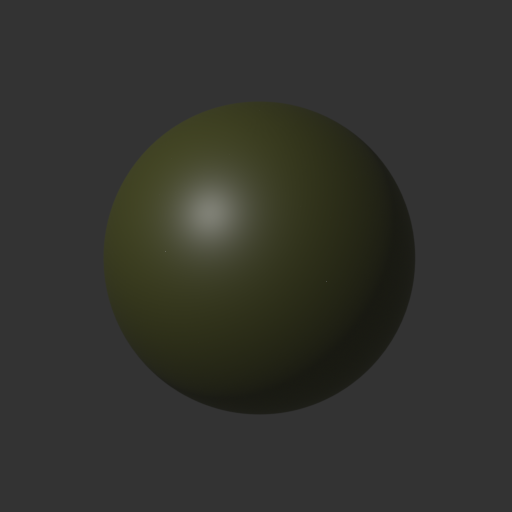
\includegraphics[width=0.1\textwidth]{interp/real_world_img/dino/base_00} & 
  % 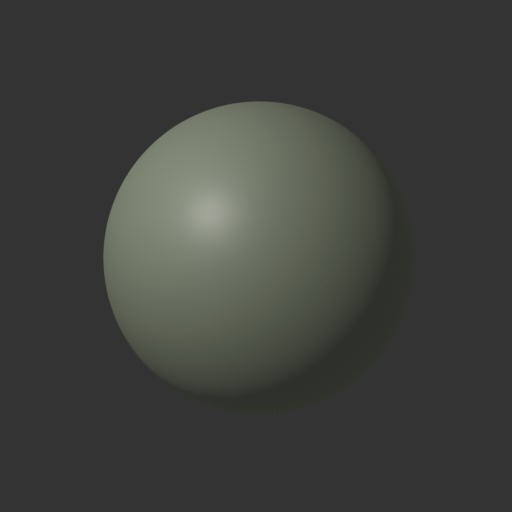
\includegraphics[width=0.1\textwidth]{interp/real_world_img/dino/base_01} & 
  % \includegraphics[width=0.1\textwidth]{interp/real_world_img/dino/base_02} &
  % \includegraphics[width=0.1\textwidth]{interp/real_world_img/house/base_00} &
  % \includegraphics[width=0.1\textwidth]{interp/real_world_img/house/base_01} & \\
  \multicolumn{3}{c}{(d). cup} & \multicolumn{3}{c}{(e). dino} & \multicolumn{3}{c}{(f). house} \\
  \multicolumn{3}{l}{\includegraphics[width=0.33\textwidth]{interp/real_world_img/pot/pot}} &
  \multicolumn{3}{l}{\includegraphics[width=0.33\textwidth]{interp/real_world_img/statue/statue}} &
  \multicolumn{3}{l}{\includegraphics[width=0.33\textwidth]{interp/real_world_img/vase/vase}}\\
  % \includegraphics[width=0.1\textwidth]{interp/real_world_img/pot/base_00} &
  % \includegraphics[width=0.1\textwidth]{interp/real_world_img/pot/base_01} & &
  % \includegraphics[width=0.1\textwidth]{interp/real_world_img/statue/base_00} & & &
  % \includegraphics[width=0.1\textwidth]{interp/real_world_img/vase/base_00} &
  % \includegraphics[width=0.1\textwidth]{interp/real_world_img/vase/base_01}\\
  \multicolumn{3}{c}{(g). pot} & \multicolumn{3}{c}{(h). statue} & \multicolumn{3}{c}{(i). vase} \\
  \end{tabular}
  \caption{Images of the real-world objects.}
  \label{fig:real_data_material}
\end{table}

\section{Parameters of real-world objects}
\begin{table}[!htbp]
  \centering
  \begin{tabular}{*{3}{p{8mm}}*{2}{p{15mm}}|r}
  \toprule
  % & & & & & \multicolumn{3}{c}{Metrics}\\
  Class & Texture & Albedo & Specularity & Roughness & Mapping\\
  \midrule
  box & 0.8 & 0.8 & 0.2 & 0.8 & PMVS, EPS, GSL\\
  cat0 & 0.5 & 0.5 & 0.2 & 0.2 & PMVS\\
  cat1 & 0.2 & 0.2 & 0.2 & 0.2 & None\\
  cup & 0.2 & 0.8 & 0.5 & 0.2 & EPS, GSL\\
  dino & 0.2 & 0.5, 0.8 & 0.2 & 0.8 & EPS, GSL\\
  house & 0.8 & 0.2, 0.8 & 0.2 & 0.2 & PMVS, GSL\\
  pot & 0.8 & 0.2, 0.5 & 0.2 & 0.2 & PMVS\\
  status & 0.2 & 0.8 & 0.2 & 0.8 & EPS, GSL\\
  vase & 0.8 & 0.2, 0.5 & 0.5 & 0.2 & PMVS\\
  \bottomrule
  \end{tabular}
  \caption{Property list for the real-world objects}
  \label{tab:real_data_prop_list}
\end{table}

\section{Results of real-world objects}
\begin{figure}[!htbp]
\centering
\begin{tabular}{l|cccc}
Mapping & PMVS & EPS & GSL & VH (BL)\\
\midrule
PMVS, EPS, GSL &
\fcolorbox{green}{white}{\raisebox{-.5\height}{\includegraphics[width=0.2\textwidth]{interp/real_interp/box/box_mvs}}}&
\fcolorbox{green}{white}{\raisebox{-.5\height}{\includegraphics[width=0.2\textwidth]{interp/real_interp/box/box_ps}}}&
\fcolorbox{green}{white}{\raisebox{-.5\height}{\includegraphics[width=0.2\textwidth]{interp/real_interp/box/box_sl}}}&
\raisebox{-.5\height}{\includegraphics[width=0.2\textwidth]{interp/real_interp/box/box_sc}}\\
PMVS &
\fcolorbox{green}{white}{\raisebox{-.5\height}{\includegraphics[width=0.2\textwidth]{interp/real_interp/cat0/cat0_mvs}}}&
\raisebox{-.5\height}{\includegraphics[width=0.2\textwidth]{interp/real_interp/cat0/cat0_ps}}&
\raisebox{-.5\height}{\includegraphics[width=0.2\textwidth]{interp/real_interp/cat0/cat0_sl}}&
\raisebox{-.5\height}{\includegraphics[width=0.2\textwidth]{interp/real_interp/cat0/cat0_sc}}\\
None &
\raisebox{-.5\height}{\includegraphics[width=0.2\textwidth]{interp/real_interp/cat1/cat1_mvs}}&
\raisebox{-.5\height}{\includegraphics[width=0.2\textwidth]{interp/real_interp/cat1/cat1_ps}}&
\raisebox{-.5\height}{\includegraphics[width=0.2\textwidth]{interp/real_interp/cat1/cat1_sl}}&
\raisebox{-.5\height}{\includegraphics[width=0.2\textwidth]{interp/real_interp/cat1/cat1_sc}}\\
EPS, GSL &
\raisebox{-.5\height}{\includegraphics[width=0.2\textwidth]{interp/real_interp/cup/cup_mvs}}&
\fcolorbox{green}{white}{\raisebox{-.5\height}{\includegraphics[width=0.2\textwidth]{interp/real_interp/cup/cup_ps}}}&
\fcolorbox{green}{white}{\raisebox{-.5\height}{\includegraphics[width=0.2\textwidth]{interp/real_interp/cup/cup_sl}}}&
\raisebox{-.5\height}{\includegraphics[width=0.2\textwidth]{interp/real_interp/cup/cup_sc}}\\
EPS, GSL &
\raisebox{-.5\height}{\includegraphics[width=0.2\textwidth]{interp/real_interp/dino/dino_mvs}}&
\fcolorbox{green}{white}{\raisebox{-.5\height}{\includegraphics[width=0.2\textwidth]{interp/real_interp/dino/dino_ps}}}&
\fcolorbox{green}{white}{\raisebox{-.5\height}{\includegraphics[width=0.2\textwidth]{interp/real_interp/dino/dino_sl}}}&
\raisebox{-.5\height}{\includegraphics[width=0.2\textwidth]{interp/real_interp/dino/dino_sc}}\\
PMVS, GSL &
\fcolorbox{green}{white}{\raisebox{-.5\height}{\includegraphics[width=0.2\textwidth]{interp/real_interp/house/house_mvs}}}&
\raisebox{-.5\height}{\includegraphics[width=0.2\textwidth]{interp/real_interp/house/house_ps}}&
\fcolorbox{green}{white}{\raisebox{-.5\height}{\includegraphics[width=0.2\textwidth]{interp/real_interp/house/house_sl}}}&
\raisebox{-.5\height}{\includegraphics[width=0.2\textwidth]{interp/real_interp/house/house_sc}}\\
\bottomrule
\end{tabular}
\caption{Reconstruction results of MVS, PS, SL, and the baseline method VH.}
\label{fig:test_real_world_img}
\end{figure}

\begin{figure}[h!]
\centering
\begin{tabular}{l|cccc}
Mapping & PMVS & Example-based PS & Gray SL & VH(BL)\\
\midrule
PMVS &
\fcolorbox{green}{white}{\raisebox{-.5\height}{\includegraphics[width=0.2\textwidth]{interp/real_interp/pot/pot_mvs}}}&
\raisebox{-.5\height}{\includegraphics[width=0.2\textwidth]{interp/real_interp/pot/pot_ps}}&
\raisebox{-.5\height}{\includegraphics[width=0.2\textwidth]{interp/real_interp/pot/pot_sl}}&
\raisebox{-.5\height}{\includegraphics[width=0.2\textwidth]{interp/real_interp/pot/pot_sc}}\\
EPS, GSL &
\raisebox{-.5\height}{\includegraphics[width=0.2\textwidth]{interp/real_interp/statue/statue_mvs}}&
\fcolorbox{green}{white}{\raisebox{-.5\height}{\includegraphics[width=0.2\textwidth]{interp/real_interp/statue/statue_ps}}}&
\fcolorbox{green}{white}{\raisebox{-.5\height}{\includegraphics[width=0.2\textwidth]{interp/real_interp/statue/statue_sl}}}&
\raisebox{-.5\height}{\includegraphics[width=0.2\textwidth]{interp/real_interp/statue/statue_sc}}\\
PMVS &
\fcolorbox{green}{white}{\raisebox{-.5\height}{\includegraphics[width=0.2\textwidth]{interp/real_interp/vase/vase_mvs}}}&
\raisebox{-.5\height}{\includegraphics[width=0.2\textwidth]{interp/real_interp/vase/vase_ps}}&
\raisebox{-.5\height}{\includegraphics[width=0.2\textwidth]{interp/real_interp/vase/vase_sl}}&
\raisebox{-.5\height}{\includegraphics[width=0.2\textwidth]{interp/real_interp/vase/vase_sc}}\\
\bottomrule
\end{tabular}
\caption{Reconstruction results of MVS, PS, SL, and the baseline method VH (cont'd).}
\label{fig:test_real_world_img}
\end{figure}

\backmatter
%    7. Index
% See the makeindex package: the following page provides a quick overview
% <http://www.image.ufl.edu/help/latex/latex_indexes.shtml>


\end{document}
